% Twoside implica che i capitoli inizino sempre con la prima pagina a sinistra, eventualmente lasciando una pagina vuota nel capitolo precedente. 
\documentclass[a4paper, twoside,openright]{report}

% Dimensione dei margini
\usepackage[a4paper,top=3cm,bottom=3cm,left=3cm,right=3cm]{geometry} 
% Dimensione del font
\usepackage[fontsize=13pt]{scrextend}
% Lingua del testo
\usepackage[english,italian]{babel}
% Lingua per la bibliografia
\usepackage[fixlanguage]{babelbib}
% Codifica del testo
\usepackage[utf8]{inputenc} 
% Encoding del testo
\usepackage[T1]{fontenc}
% Per modificare l'header delle pagine 
\usepackage{fancyhdr}               

\usepackage{float}

% Librerie matematiche
\usepackage{amssymb}
\usepackage{amsmath}
\usepackage{amsthm}         

% Uso delle immagini
\usepackage{graphicx}
% Uso dei colori
\usepackage[dvipsnames]{xcolor}         
% Uso dei listing per il codice
\usepackage{listings}          
% Per inserire gli hyperlinks tra i vari elementi del testo 
\usepackage{hyperref}     
% Diversi tipi di sottolineature
\usepackage[normalem]{ulem}

% -----------------------------------------------------------------

% Modifica lo stile dell'header
\pagestyle{fancy}
\fancyhf{}
\lhead{\rightmark}
\rhead{\textbf{\thepage}}
\fancyfoot{}
\setlength{\headheight}{16pt}

% Rimuove il numero di pagina all'inizio dei capitoli
\fancypagestyle{plain}{
  \fancyfoot{}
  \fancyhead{}
  \renewcommand{\headrulewidth}{0pt}
}

\definecolor{backcolour}{rgb}{0.90,0.95,0.92}

% Stile del codice
% \lstset{style=codeStyle}
\lstdefinestyle{codeStyle}{
    backgroundcolor=\color{backcolour},
    commentstyle=\color{teal},
    keywordstyle=\color{Magenta},
    numberstyle=\tiny\color{gray},
    stringstyle=\color{violet},
    basicstyle=\ttfamily\scriptsize,
    breakatwhitespace=false,     
    breaklines=true,                 
    captionpos=b,                    
    keepspaces=true,                 
    numbers=left,                    
    numbersep=5pt,                  
    showspaces=false,                
    showstringspaces=false,
    showtabs=false,
    tabsize=1
} \lstset{style=codeStyle}

% \lstset{style=longBlock}
\lstdefinestyle{longBlock}{
    commentstyle=\color{teal},
    keywordstyle=\color{Magenta},
    numberstyle=\tiny\color{gray},
    stringstyle=\color{violet},
    basicstyle=\ttfamily\scriptsize,
    breakatwhitespace=false,         
    breaklines=true,                 
    captionpos=b,                    
    keepspaces=true,                 
    numbers=left,                    
    numbersep=5pt,                  
    showspaces=false,                
    showstringspaces=false,
    showtabs=false,                  
    tabsize=2
} \lstset{style=codeStyle}

% Togliendo il commento al comando che segue, si inseriscono nella bibliografia anche le fonti presenti in Bibliography.bib ma non citati direttamente con il comando \cite
\nocite{*}

% Margini prima e dopo blocchi di codice, per avere più distanza
\lstset{aboveskip=20pt,belowskip=20pt}

% Modifica dello stile dei riferimenti
\hypersetup{
    colorlinks,
    linkcolor=black,
    citecolor=black
}

% Aggiunti definizioni, teoremi, linea e listing
\newtheorem{definition}{Definizione}[section]
\newtheorem{theorem}{Teorema}[section]
\providecommand*\definitionautorefname{Definizione}
\providecommand*\theoremautorefname{Teorema}
\providecommand*{\listingautorefname}{Listing}
\providecommand*\lstnumberautorefname{Linea}

\raggedbottom



% -----------------------------------------------------------------
\begin{document}
\begin{titlepage}
\begin{figure}[!htb]
    \centering
\end{figure}
\vspace{30mm}
\begin{center}
    \LARGE{UNIVERSITÀ DEGLI STUDI DI MODENA E REGGIO EMILIA}
    \vspace{5mm}
    \\ \large{DIPARTIMENTO DI INGEGNERIA "ENZO FERRARI"}
    \vspace{5mm}
    \\ Laurea Magistrale in Ingegneria Informatica
\end{center}

\vspace{15mm}
\begin{center}
    {\LARGE{\bf NextPyter: una piattaforma distribuita per Jupyter Notebooks }}
    
    % Se il titolo è abbastanza corto da stare su una riga, si può usare
    
    % {\LARGE{\bf Un fantastico titolo per la mia tesi!}}
\end{center}
\vspace{30mm}

\begin{minipage}[t]{0.47\textwidth}
	{\large{Relatore:}{\normalsize\vspace{3mm}
	\bf\\ \large{Prof: Claudia Canali} \normalsize\vspace{3mm}\bf \\ \large{Prof: Francesco Faenza}}}
\end{minipage}
\hfill
\begin{minipage}[t]{0.47\textwidth}\raggedleft
	{\large{Candidato:}{\normalsize\vspace{3mm} \bf\\ \large{Emiliano Maccaferri}}}
\end{minipage}

\vspace{30mm}
\hrulefill
\\\centering{\large{Anno Accademico 2023/2024}}

\end{titlepage}
\let\cleardoublepage\clearpage
\dedication{\textit{
    Dediche:\newline
    A Eleonora e alla sua immensa presenza in tutte le mie vite.\newline
    Ai miei genitori, sempre al mio fianco, senza mai chiedere niente in cambio.\newline
    A Barbara, Tiziano, Leonardo, Marcello e Michele, la mia seconda famiglia. 
}}
\newpage

\section*{Ringraziamenti}
Voglio ringraziare immensamente tutto il personale del CRIS per la loro calorosità e disponibilità durante il mio tirocinio, in particolare Francesco e Giovanni, due persone che mi hanno trasmesso la loro positività sin da subito, affiancandomi in questo bellissimo progetto, dandomi tutti gli strumenti di cui avevo bisogno, dando lustro all'istituzione che è l'Università di Modena e Reggio Emilia.
\newline
\newline
Il CRIS è molto più che un insieme di persone che fanno ricerca, in questo laboratorio ho potuto respirare quella che è veramente l'aria che dovrebbe tirare in tutte le università d'Italia: la sicurezza, nel senso emotivo, il rispetto reciproco e la totale assenza di percezione di subordinazione che una persona prova quando mette piede per la prima volta in questo splendido ambiente sono sensazioni che non ho mai provato e che faranno sicuramente da riferimento per tutte le esperienze, lavorative e non, che vorrò intraprendere nella mia vita.
\tableofcontents

\listoffigures
\chapter{Introduzione}
Il fulcro della ricerca è la collaborazione, un elemento chiave che permette di unire le più distinte competenze per affrontare questioni della più disparata natura per trovare soluzioni valide e innovative. In un ambiente di ricerca sempre più in simbiosi con le ultime tecnologie, è importante trovare validi strumenti che permettano di sfruttarle al meglio, rendendo il processo di ricerca quanto più proficuo possibile.
\newline
\newline
Nella ricerca che si basa sull’analisi di dati assistita da calcolatori, uno degli strumenti più diffusi è sicuramente JupyterLab, un ambiente computazionale che permette di utilizzare svariati linguaggi di programmazione a supporto delle proprie attività di ricerca, permettendo a ricercatrici e ricercatori di condividere i propri esperimenti e analisi in maniera estremamente facile e riproducibile.
\newline
Lo scopo di questa tesi è quello di proporre NextPyter, una piattaforma che si pone come obiettivo quello di rendere accessibile a chiunque l’utilizzo di uno strumento come JupyterLab, integrando funzioni come la condivisione di file, supporto alla multiutenza, sicurezza e semplicità d’uso, tutte dal proprio browser.
\newline
Sfruttando le ultime tecnologie di containerizzazione come Kubernetes e Docker, l'obiettivo di NextPyter è quello di creare un'interfaccia completamente platform agnostic, tramite la quale sarà possibile gestire il ciclo di vita dei vari Jupyter notebook che saranno presenti nel sistema. NextPyter sarà eventualmente accoppiato ad un sistema di gestione e condivisione file, Nextcloud, per permettere la collaborazione tra gruppi di ricerca in maniera particolarmente semplice.
\newline
Nel secondo capitolo verrà fatta una breve introduzione alle pratiche di ricerca mediante l'utilizzo di notebook computazionali e di come queste ultime possono essere integrate con piattaforme di \textit{storage cloud based} e non.
\newline
Nel terzo capitolo, oltre ad un breve excursus sulla versione \textit{legacy} di NextPyter, sarà descritta la progettazione della piattaforma NextPyter, dove verrà delineato lo schema tecnico che verrà seguito, poi, nel quarto capitolo, che commenterà e dettaglierà l'effettiva realizzazione della piattaforma.
\newline
Nel quinto capitolo verranno proposte le conclusioni e gli sviluppi futuri per la piattaforma.
\chapter{Ricerca collaborativa con notebook computazionali e piattaforme di condivisione file}
I notebook computazionali non sono altro che un insieme di strumenti e programmi che permettono la creazione, condivisione e riproduzione di ambienti di sviluppo in maniera estremamente semplice. Queste \textit{suite} sono ampiamente utilizzate in tantissimi contesti, non solo nella ricerca, che fanno affidamento al calcolo numerico, come l'intelligenza artificiale, la \textit{data analysis}, la simulazione o comunque tutti gli scenari nei quali siano presenti, sostanzialmente, codice, dati e bisogno di riproducibilità da parte di altri utenti.
\newline
Ovviamente, i casi d'uso di notebook computazionali possono estendersi, anche più semplicemente (ma con, forse, anche più rilevanza rispetto ai casi specificati poc'anzi), alla didattica: basti pensare al caso in cui una docente di informatica voglia condividere un esercizio con gli studenti senza che questi ultimi debbano installare il supporto al linguaggio di programmazione nel quale l'esercizio stesso è scritto, oppure al caso in cui una studentessa di matematica voglia condividere risultati di analisi statistiche con il proprio docente, allegando, in un unico ambiente, dati, codice e risultati.
\newline
I notebook computazionali semplificano notevolmente questi processi, perché si occupano di una serie di problemi di natura puramente "operazionale", ovvero tutti quei processi, ripetitivi, che vengono eseguiti per generare un ambiente nel quale lavorare ed eseguire codice, che, generalmente, non interessano (e non dovrebbero interessare) gli utenti di tali strumenti, che magari vogliono semplicemente eseguire l'ambiente senza troppe domande, anche perché, molto spesso, gli utenti finali di questi notebook non sono, necessariamente, persone con avanzate capacità informatiche. Questo è un altro punto fondamentale: chi scrive codice, specialmente nella ricerca, non è necessariamente uno studente di informatica, ma può essere una professoressa di geologia che deve consultare delle analisi numeriche fatte da un collega, un professore di Controlli Automatici che vuole eseguire uno script Matlab, insomma, persone per le quali l'informatica è un servizio: i notebook computazionali permettono a chiunque di accedere, in maniera estremamente semplificata, alle potenzialità di ambienti numerici avanzati senza il costo operativo.

\section{JupyterLab}
JupyterLab\footnote{https://jupyter.org/} è una \textit{suite} di strumenti basata su Jupyter Notebook, che permette di utilizzare notebook computazionali direttamente dal proprio browser.
\begin{figure}[h]
    \centering
    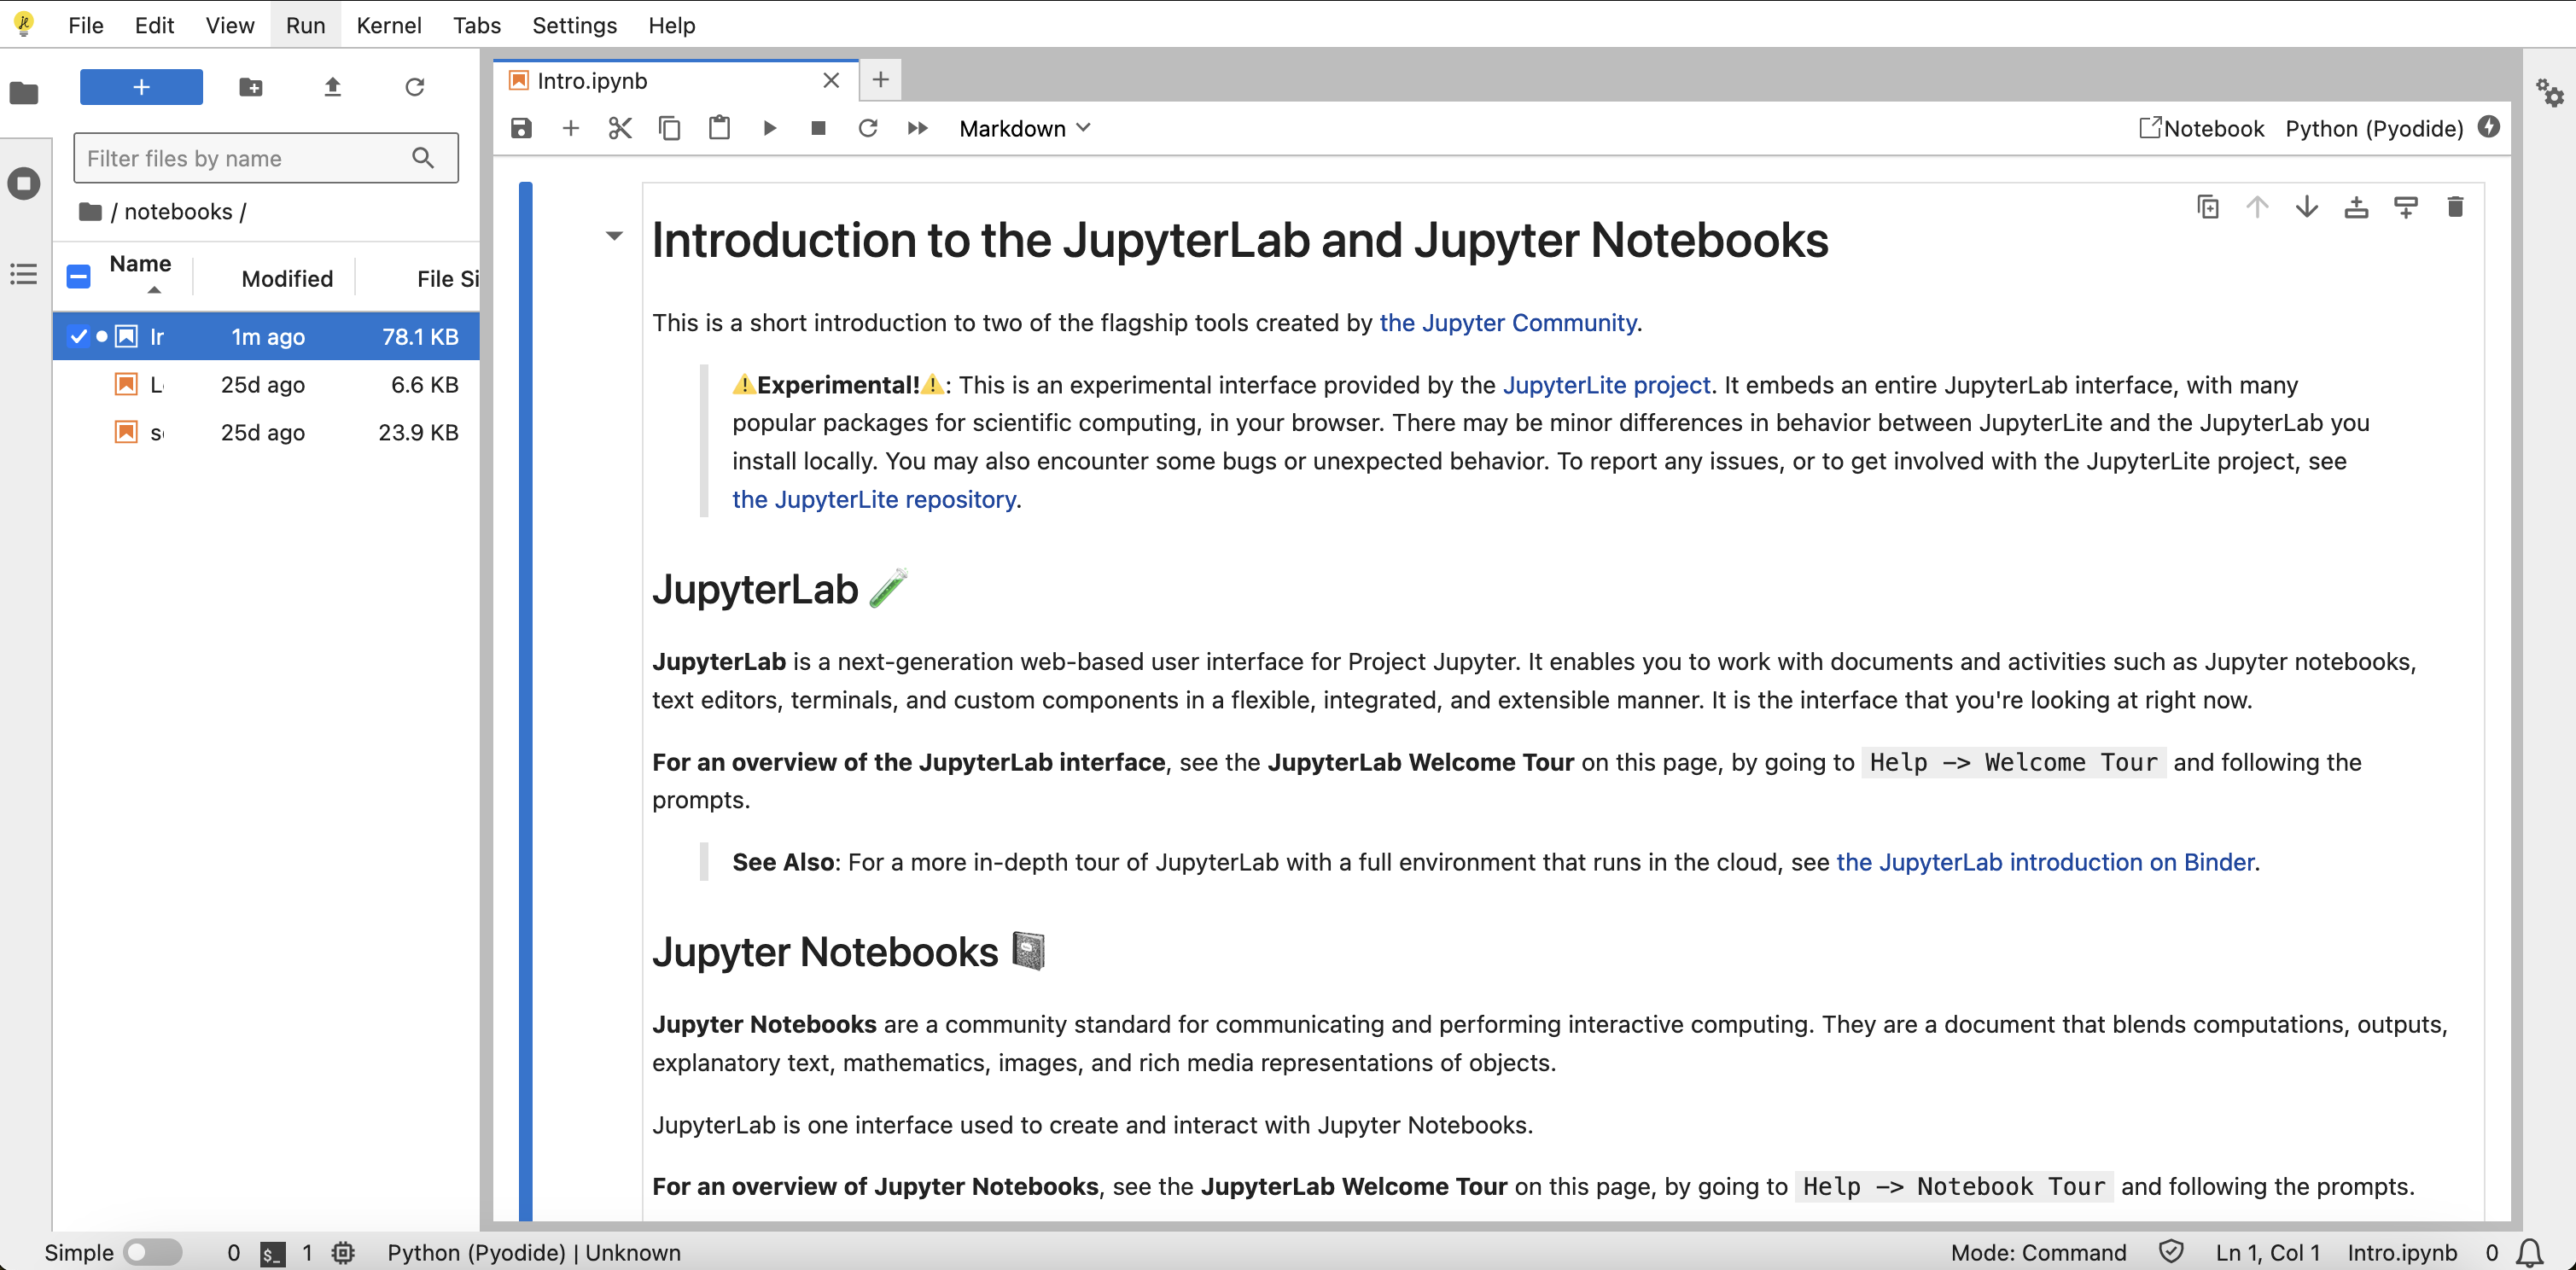
\includegraphics[width=0.75\textwidth]{images/jupyter-hub-1.png}
    \caption{Interfaccia di JupyterLab}
    \label{fig:jupyter-interface-1}
\end{figure}
\newline
JupyterLab si pone l'obiettivo di essere la piattaforma \textit{all-in-one} che permette di utilizzare in maniera più semplice l'ambiente precedente (Jupyter Notebook): l'interfaccia, visibile in figura \ref{fig:jupyter-interface-1}, è la stessa, infatti. 

\subsection{Funzionalità base di JupyterLab}
\subsubsection{Kernel Jupyter}
I kernel Jupyter\footnote{https://docs.jupyter.org/en/latest/projects/kernels.html} non sono altro che l'implementazione dei linguaggi di programmazione che possono essere utilizzati all'interno di un Jupyter Notebook, rendendo questo genere di ambienti estremamente estensibili. A rafforzare l'estensibilità di Jupyter, vi è il fatto che il framework utilizzato per implementare kernel, Xeus\footnote{https://xeus.readthedocs.io/en/latest/}, sia completamente \textit{open source}, rendendo, di fatto, realizzabili kernel per qualsiasi linguaggio di programmazione. Proprio per questo motivo, JupyterLab può vantare di una lunga lista di kernel disponibili\footnote{https://github.com/jupyter/jupyter/wiki/Jupyter-kernels}, tra i quali figurano Python, MatLab, Wolfram Mathematica, Gnuplot e molti altri.
\subsubsection{Creazione di un notebook}
Tramite la demo disponibile sul sito ufficiale\footnote{https://jupyter.org/try-jupyter/lab/}, è possibile interagire con un ambiente JupyterHub pre-impostato.
\newline
Per creare un notebook, basterà premere sul pulsante blu in alto a sinistra e selezionare l'ambiente Python per i notebook, come si può vedere in figura \ref{fig:jupyter-interface-2}.
\begin{figure}[h]
    \centering
    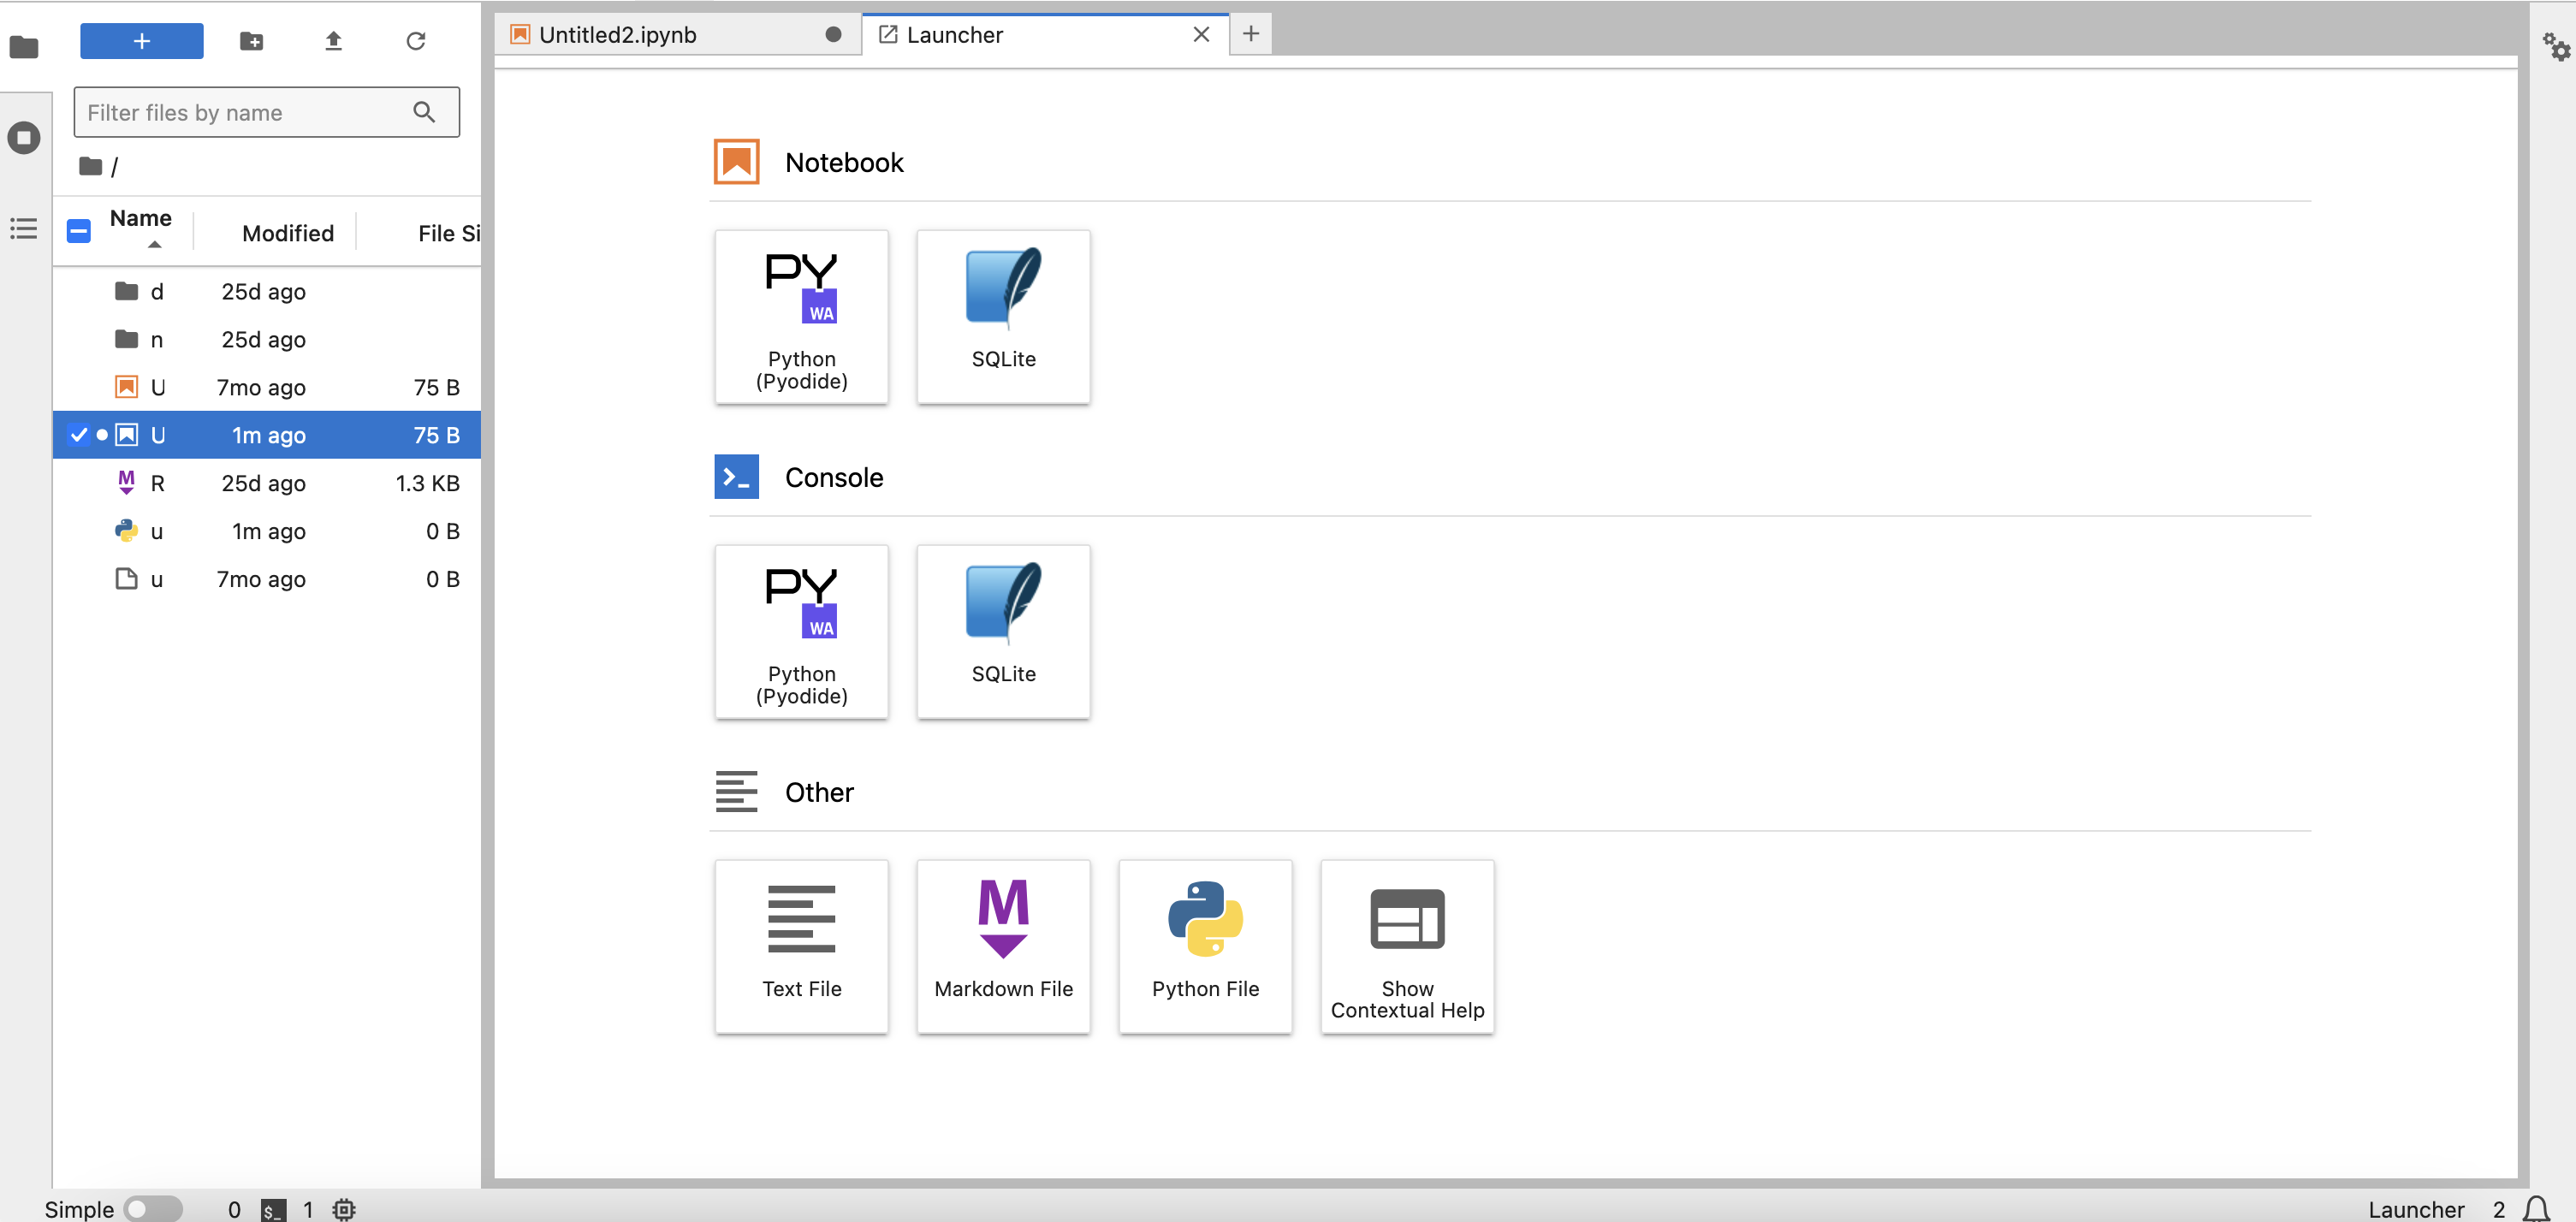
\includegraphics[width=0.75\textwidth]{images/jupyter-hub-2.png}
    \caption{Creazione di un notebook Python}
    \label{fig:jupyter-interface-2}
\end{figure}
\newline
Una volta creato il notebook, è possibile eseguire codice Python arbitrario al suo interno senza nessun problema (figura \ref{fig:jupyter-interface-3}).
\begin{figure}[h]
    \centering
    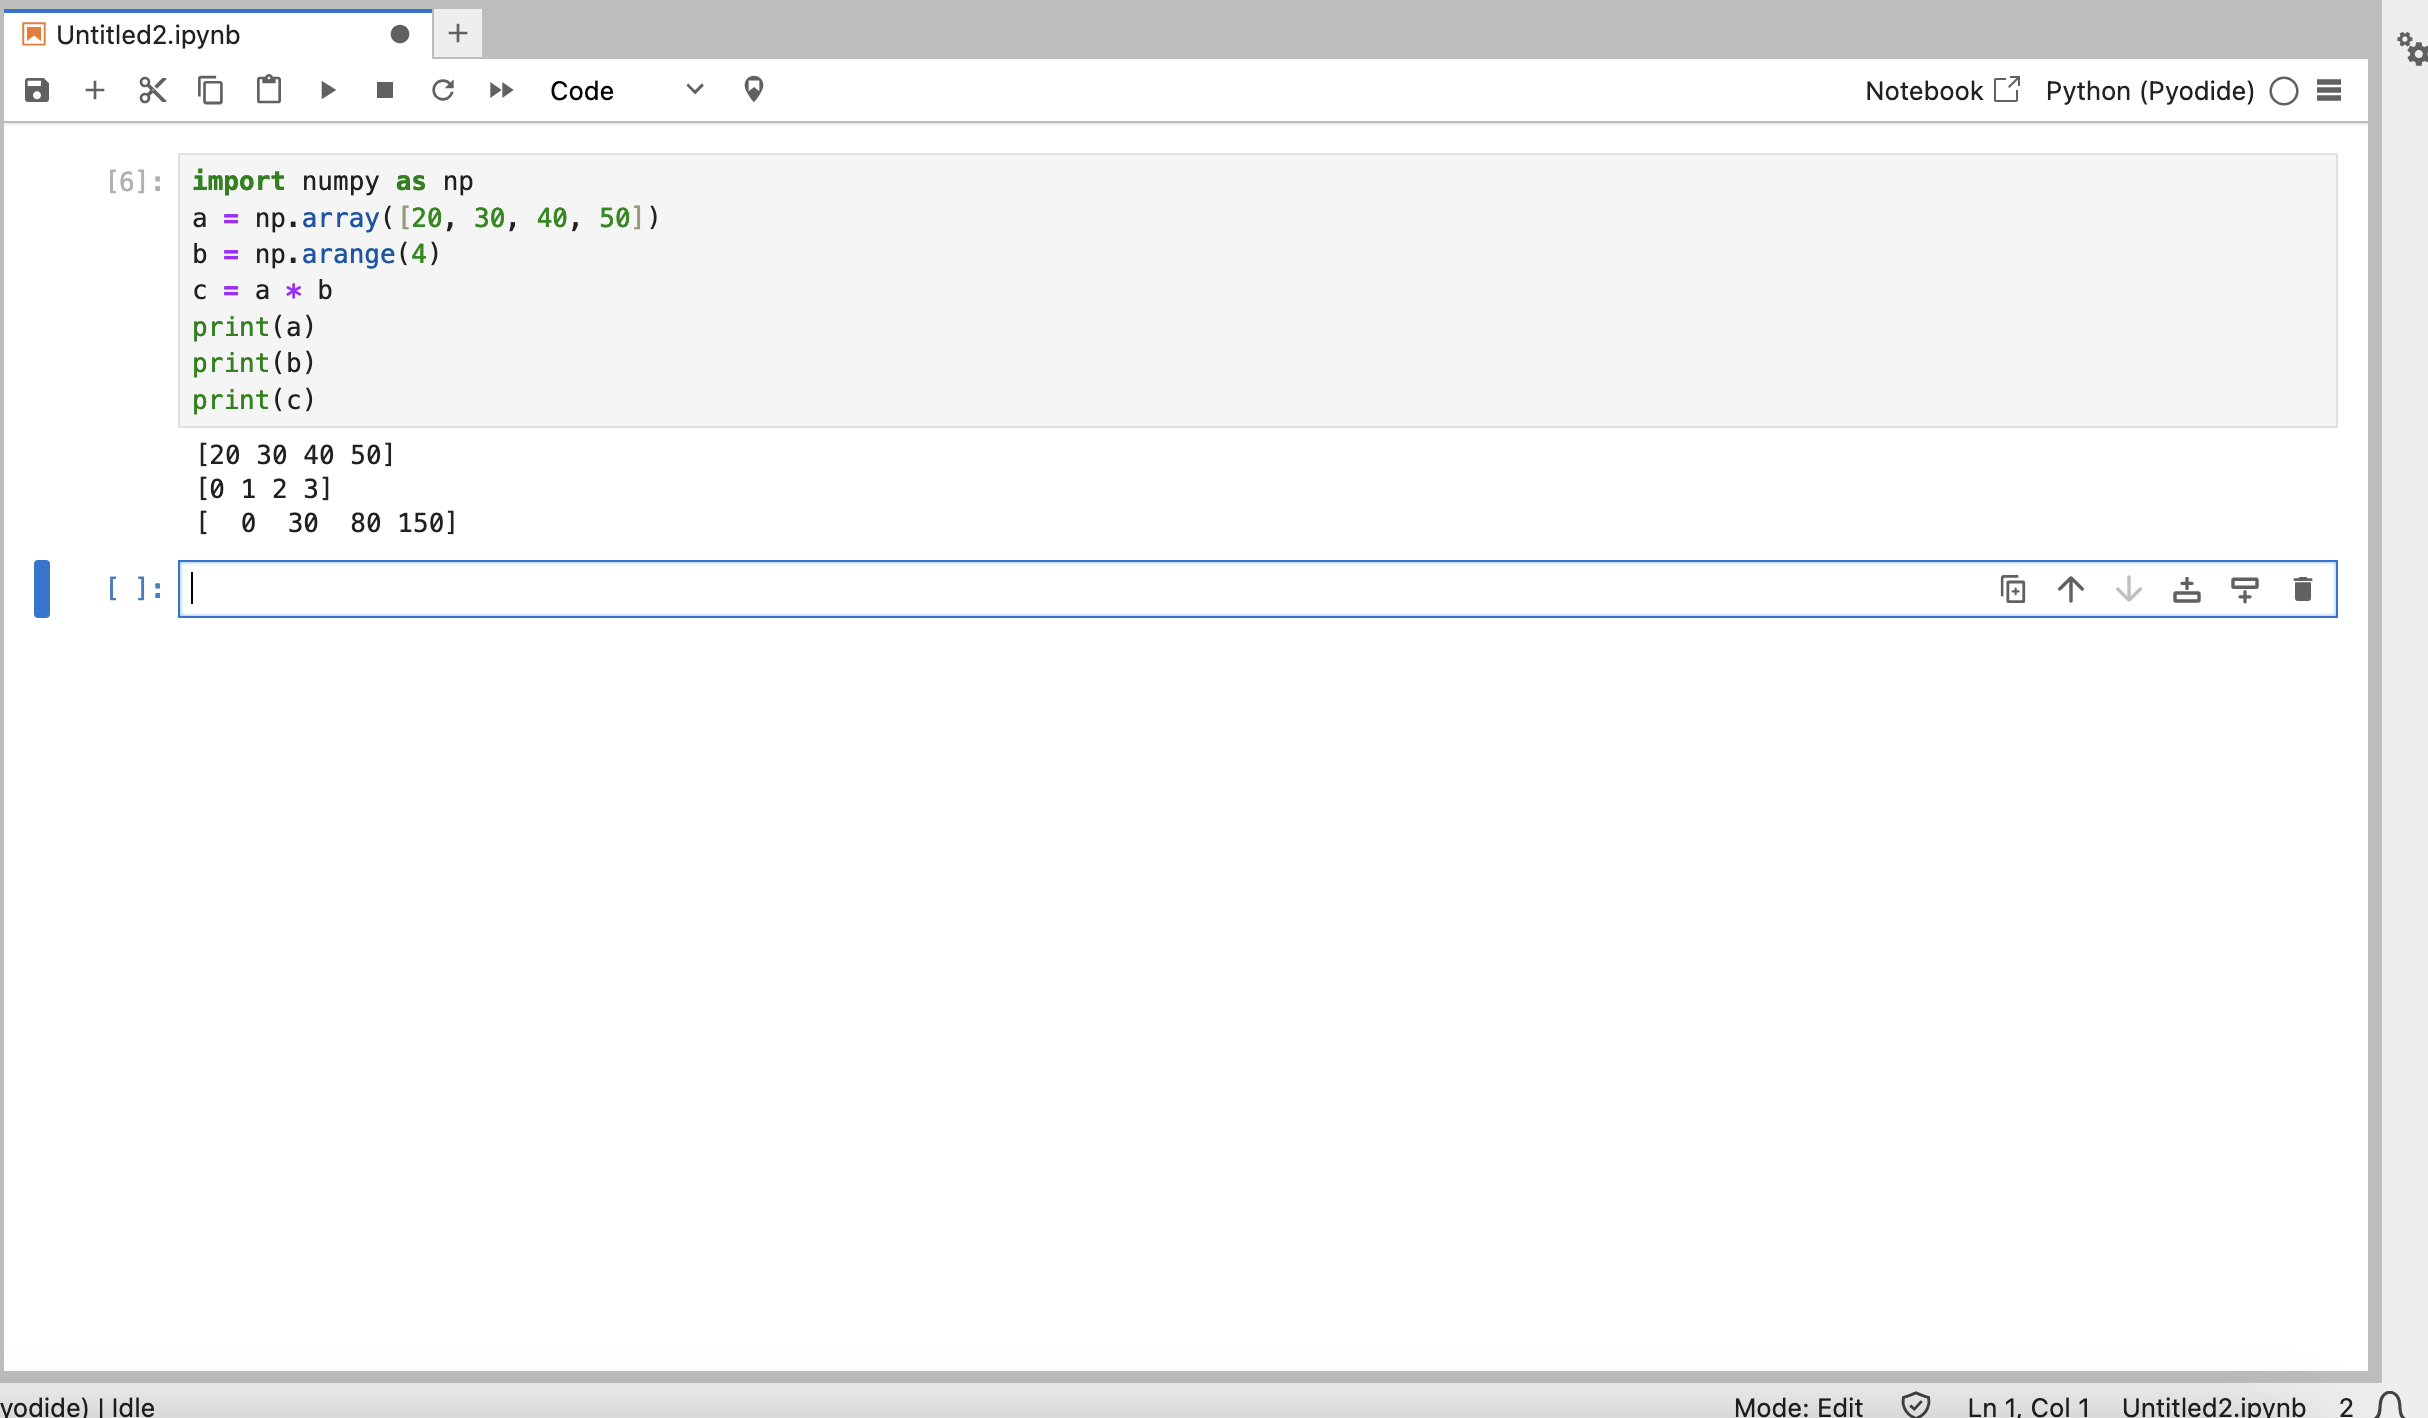
\includegraphics[width=0.75\textwidth]{images/jupyter-hub-3.png}
    \caption{Esecuzione codice Python in un notebook}
    \label{fig:jupyter-interface-3}
\end{figure}
\newpage
\section{Condivisione file}
È naturale che gruppi di ricerca, numerosi o meno che siano, necessitino di piattaforme su cui condividere e scambiare file in maniera veloce ed efficiente. L'accesso a questi file, poi, dovrà seguire un sistema di permessi, che permetterà a utenti con determinati privilegi di poter accedere o meno ai file in questione.\newline
Piattaforme di condivisione file come \textit{Google Drive}\footnote{https://drive.google.com} soddisfano sicuramente questo genere di requisiti, ma potrebbero non essere particolarmente adatte all'ambito accademico, principalmente per questioni riguardanti gli elevati costi di \textit{storage} e la privacy dei dati.
\newline
Sovente, infatti, le università scelgono di implementare \textit{in house} il proprio sistema di archiviazione e dematerializzazione dati, proprio per sopperire ai problemi succitati. Per questo motivo, l'utilizzo di piattaforme \textit{self-hosted} può sicuramente rappresentare una via percorribile per la gestione dei file senza ricorrere all'utilizzo di software commerciali gestiti esternamente.

\section{Nextcloud}
Nextcloud\footnote{https://nextcloud.com/} è una piattaforma \textit{open source} per la sincronizzazione e la condivisione di file, progettata per fornire un'alternativa autonoma ai servizi di cloud storage gestiti da terze parti. L'interfaccia utente è assolutamente familiare, anche ai più digiuni di informatica, rendendo l'esperienza utente e l'\textit{onboarding} di nuovi utenti particolarmente semplice.

\subsection{Sviluppo di applicazioni {ad-hoc} per Nextcloud}
È possibile sviluppare, in \textit{PHP}, apposite applicazioni che si possono integrare direttamente con la propria installazione di Nextcloud, un ulteriore punto a favore per l'utilizzo di questo software in ambito accademico.
\newline
È infatti molto probabile che un'istituzione come un'università abbia un portale di accesso con credenziali unificate, abbia bisogno di supporti personalizzati per processi interni e molto altro, rendendo la scelta di una piattaforma altamente personalizzabile come Nextcloud una necessità non negoziabile. 

\newpage
\section{Sfide}
Sebbene le tecnologie succitate siano estremamente versatili e di facile utilizzo, non si può dire altrettanto della loro installazione e manutenzione. Serve adibire personale alla gestione dello spazio virtuale per i documenti, a partire dalla configurazione dei \textit{server} sui quali i documenti fisicamente risiederanno, della rete che collega tali server, fino ad arrivare all'installazione dei vari servizi e l'esposizione di questi ultimi al pubblico.\newline
Una piattaforma del genere, inoltre, dovrà fornire un grado di disponibilità (in termini di \textit{uptime}) generalmente alto, pertanto dovranno essere applicate logiche di replicazione e ridondanza che permettano un veloce recupero della stabilità del sistema nel caso di problemi dovuti a malfunzionamenti o interruzioni di servizio.
\newline
Queste sono le sfide che una piattaforma come \textit{NextPyter} si prefigge come obiettivi, per rendere la ricerca collaborativa quanto più accessibile possibile, sviluppando una soluzione che unisca la versatilità di JupyterLab alla familiarità e estensibilità di Nextcloud.
\chapter{Progettazione di \textit{NextPyter}}
Il lavoro descritto in questa tesi è il frutto di una seconda iterazione di sviluppo e cambiamenti su codice già esistente. Infatti, è stata ereditata una \textit{codebase}, che verrà indicata con il nome \textit{NextPyter "1.0"}, sulla quale era necessario effettuare modifiche per migliorare il progetto esistente, oltre che migrare la piattaforma ad una soluzione facilmente distribuibile su \textit{Kubernetes}. \newline
Verrà esplorato brevemente l'ottimo lavoro effettuato in precedenza e la sua architettura, verrà fatta un'analisi del sistema a quello stato e, successivamente, verrà descritto il passaggio da \textit{NextPyter "1.0"} a \textit{NextPyter "2.0"}, che rappresenta lo stato del progetto alla stesura di questa tesi. 
\section{Obiettivi di \textit{NextPyter}}
In generale, \textit{NextPyter} vuole essere una piattaforma tramite la quale sia possibile condividere in maniera efficiente dati e codice a scopo di ricerca. Come si può intuire dal nome, per realizzare gli obiettivi posti, \textit{NextPyter} fa uso di \textit{Nextcloud}, per la gestione dei file, e di \textit{JupyterLab}, che accederà ai file gestiti da Nextcloud.

\subsection{Containerizzazione}
Il fondamento cardine di \textit{NextPyter}, per entrambe le versioni, è la \textit{containerizzazione}, ovvero la pratica di distribuire software mediante l'utilizzo di \textit{container}\footnote{https://en.wikipedia.org/wiki/Docker\_(software)}, generalmente Docker, ambienti di esecuzione completamente isolati rispetto al resto del sistema. 
\newline
Per creare ambienti di sviluppo (i Jupyter Notebook) quanto più sicuri possibile, l'utilizzo di tecnologie di \textit{containerizzazione} è fondamentale, per la semplicità d'uso e la modularità che questo approccio offre.\newline
Tramite cosiddette \textit{immagini}\footnote{https://www.techtarget.com/searchitoperations/definition/Docker-image}, infatti, è possibile eseguire software che richiede numerose dipendenze, come \textit{JupyterLab} e lo stesso \textit{Nextcloud}, in maniera estremamente semplice, utilizzando una sorta di "pacchetto", l'immagine, per l'appunto, che viene scaricato da un registro immutabile\footnote{https://hub.docker.com}. Replicare un ambiente composto da tanti componenti complessi, quindi, è estremamente semplice, se si fa leva su tecnologie di \textit{containerizzazione}, per i vantaggi di distribuzione che questa metodologia offre.

\subsection{Interfaccia grafica familiare}
Per favorire l'utilizzo di \textit{NextPyter}, l'interfaccia deve essere quanto più semplice possibile, per ragione già specificate nell'introduzione di questa tesi. 
\newline
Per questo motivo, come già anticipato, viene usato Nextcloud come interfaccia principale, anche per via del fatto che si tratta di un'affermata soluzione \textit{self-hosted}, con una community sempre più in via di espansione \cite{nextcloud-growing}.

\subsection{Collaborazione in sicurezza}
Accoppiando tecnologie di \textit{containerizzazione} e moderni sistemi di autenticazione si vuole creare un'esperienza utente quanto più sicura possibile. \newline
Oltre alle \textit{policy} di sicurezza sulla gestione dei file che \textit{Nextcloud} già offre, l'obiettivo finale è quello di accoppiare, a ciascun utente, i permessi per creare, visualizzare e modificare determinati \textit{notebook} in maniera completamente privata, permettendo la selettiva condivisione di questi ultimi.
\newline
L'isolamento, quindi, deve avvenire non solo a livello di permesso sui file, ma anche a livello di \textit{notebook}.

\subsection{FLOSS}
Per favorire lo sviluppo di \textit{NextPyter} è stato deciso di adottare la filosofia FLOSS\footnote{https://www.gnu.org/philosophy/floss-and-foss.en.html}, \textit{Free/Libre And Open Source Software}. Il codice sorgente del progetto è pubblico e consultabile su una \textit{repository GitLab}\footnote{https://gitlab.com/nextpyter/}. Tutti i componenti sono sotto licenza \textit{MIT} e sono liberamente modificabili da chiunque voglia partecipare allo sviluppo di questa piattaforma.

\newpage

\section{NextPyter \textit{"1.0"}}
Per poter parlare dell'evoluzione della piattaforma \textit{NextPyter}, è opportuno introdurre brevemente lo stato di quest'ultima prima che iniziasse il lavoro di revisione che verrà descritto successivamente.
\newline
Per ultieriori dettagli su questa implementazione, è opportuno consultare la tesi del progetto originale \cite{nextpyter-1}.
\newline
\begin{figure}[h]
    \centering
    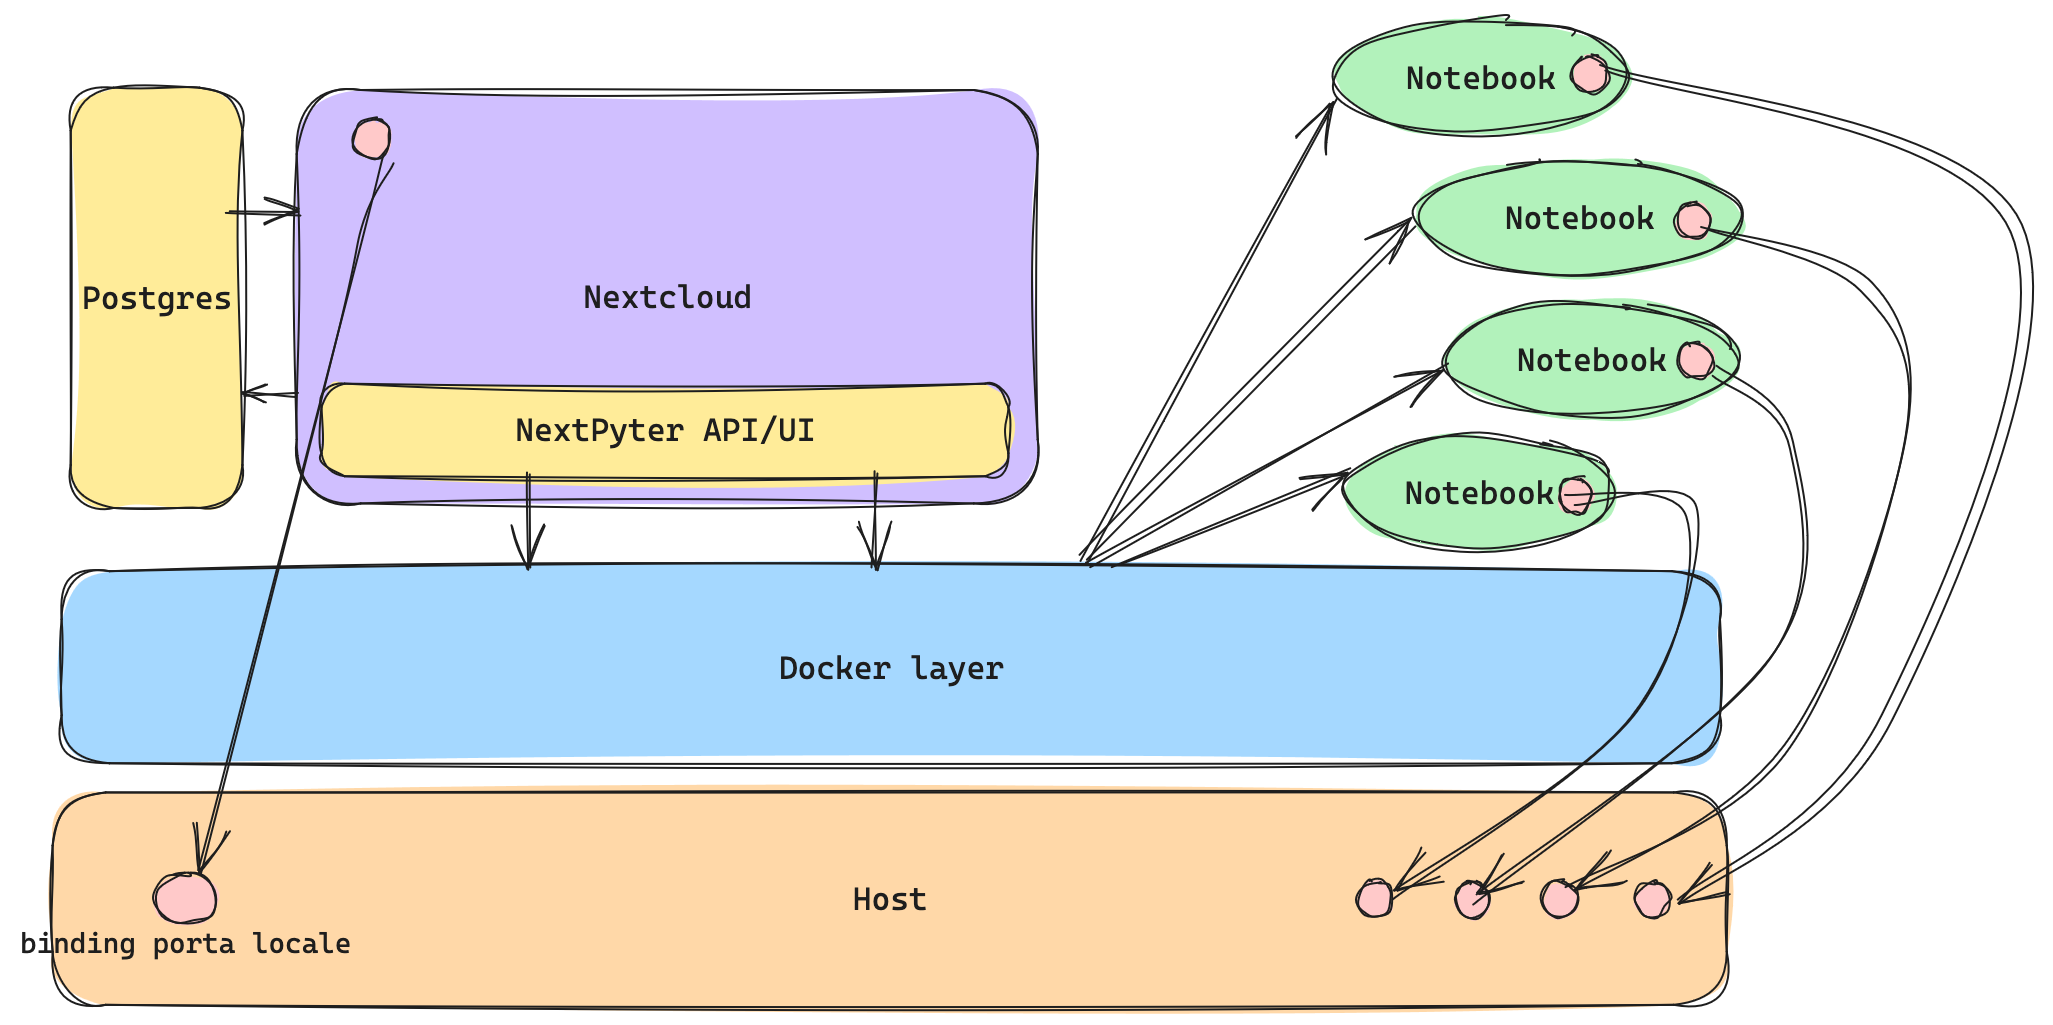
\includegraphics[width=1\textwidth]{files/images/nextpyter-1-0.png}
    \caption{Schema architetturale NextPyter "1.0"}
    \label{fig:nextpyter-1-0-architecture}
\end{figure}
\newline
In figura \ref{fig:nextpyter-1-0-architecture} è possibile vedere uno schema architetturale di alto livello della piattaforma \textit{"1.0"} e i vari componenti che la realizzano:
\begin{itemize}
    \item Un'installazione di Nextcloud e il relativo database (Postgres) che utilizza per gestire utenti, permessi e quant'altro;
    \item Un'applicazione \textbf{installata all'interno di Nextcloud}, ovvero \textit{NextPyter} vero e proprio. Questo applicativo si interfaccerà direttamente con Docker per creare e gestire i \textit{container} relativi ai notebook. Questo componente comprenderà sia un'API per l'interfaccia con Docker, che il componente relativo alla UI e alla visualizzazione dei dati;
    \item Notare che ciascun notebook avrà un \textit{binding} di una porta locale rispetto all'host sul quale Docker sta eseguendo, pertanto \textit{NextPyter} avrà bisogno di trovare una porta libera sull'host prima di creare un container: in questo modo i notebook saranno accessibili dall'esterno.
\end{itemize}
\newpage
\subsection{Funzionamento applicativo \textit{NextPyter} installato su Nextcloud}
L'applicazione installata su Nextcloud regola la creazione, l'avviamento e l'eventuale eliminazione dei notebook Jupyter da Nextcloud.
\newline
In sostanza, è possibile, tramite le estensioni fornite da \textit{NextPyter}, creare delle particolari cartelle che conterranno file relativi a determinati notebook, che verranno eseguiti effettuando determinate chiamate HTTP verso il socket di Docker stesso. 
\newline
Una volta avviato un notebook, sarà possibile accedervi mediante l'utilizzo di un token che viene generato a tempo di esecuzione dall'applicativo stesso, associato all'utente che esegue il notebook, in modo che solo chi ha tale token potrà accedere al container in questione.
\newline
A seguire, alcune immagini che illustrano il funzionamento dell'applicativo.
\newline
\begin{figure}[h]
    \centering
    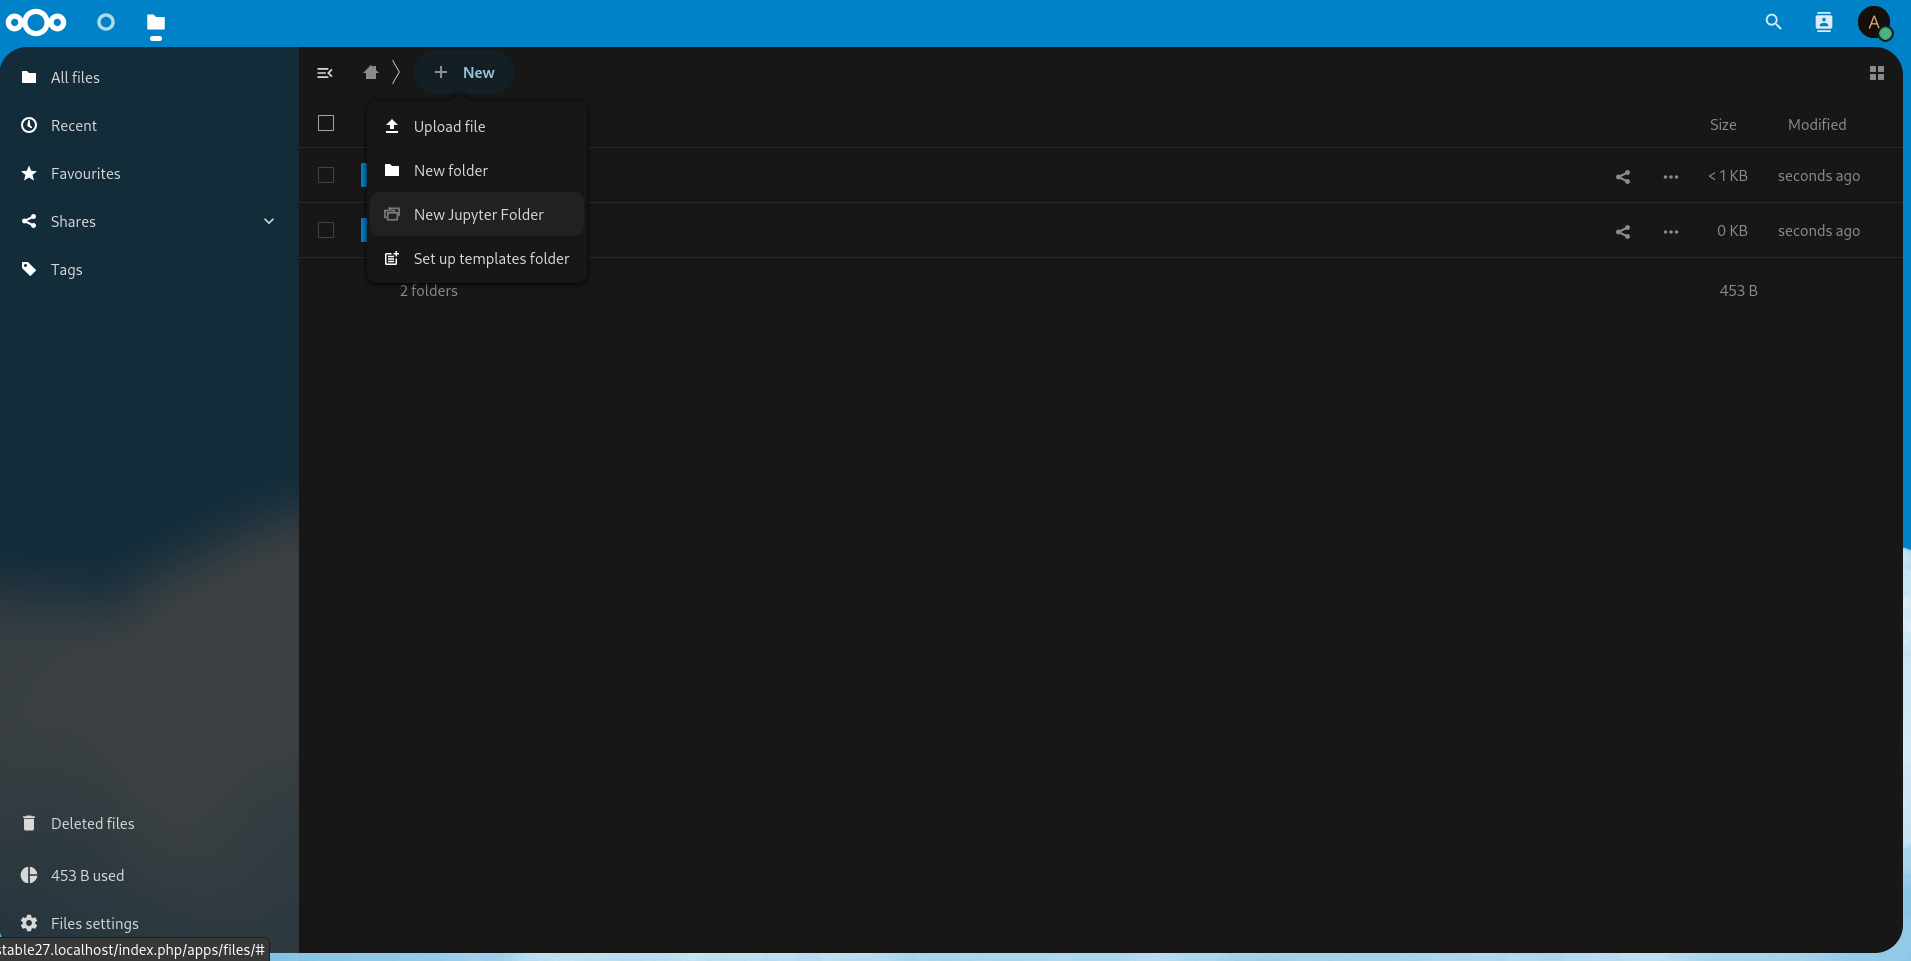
\includegraphics[width=0.75\textwidth]{files/images/example-nextpyter-1-1.png}
    \caption{Interfaccia grafica NextPyter "1.0" - Creazione cartella per notebook Jupyter}
    \label{fig:1.0-example-1}
\end{figure}
\begin{figure}[h]
    \centering
    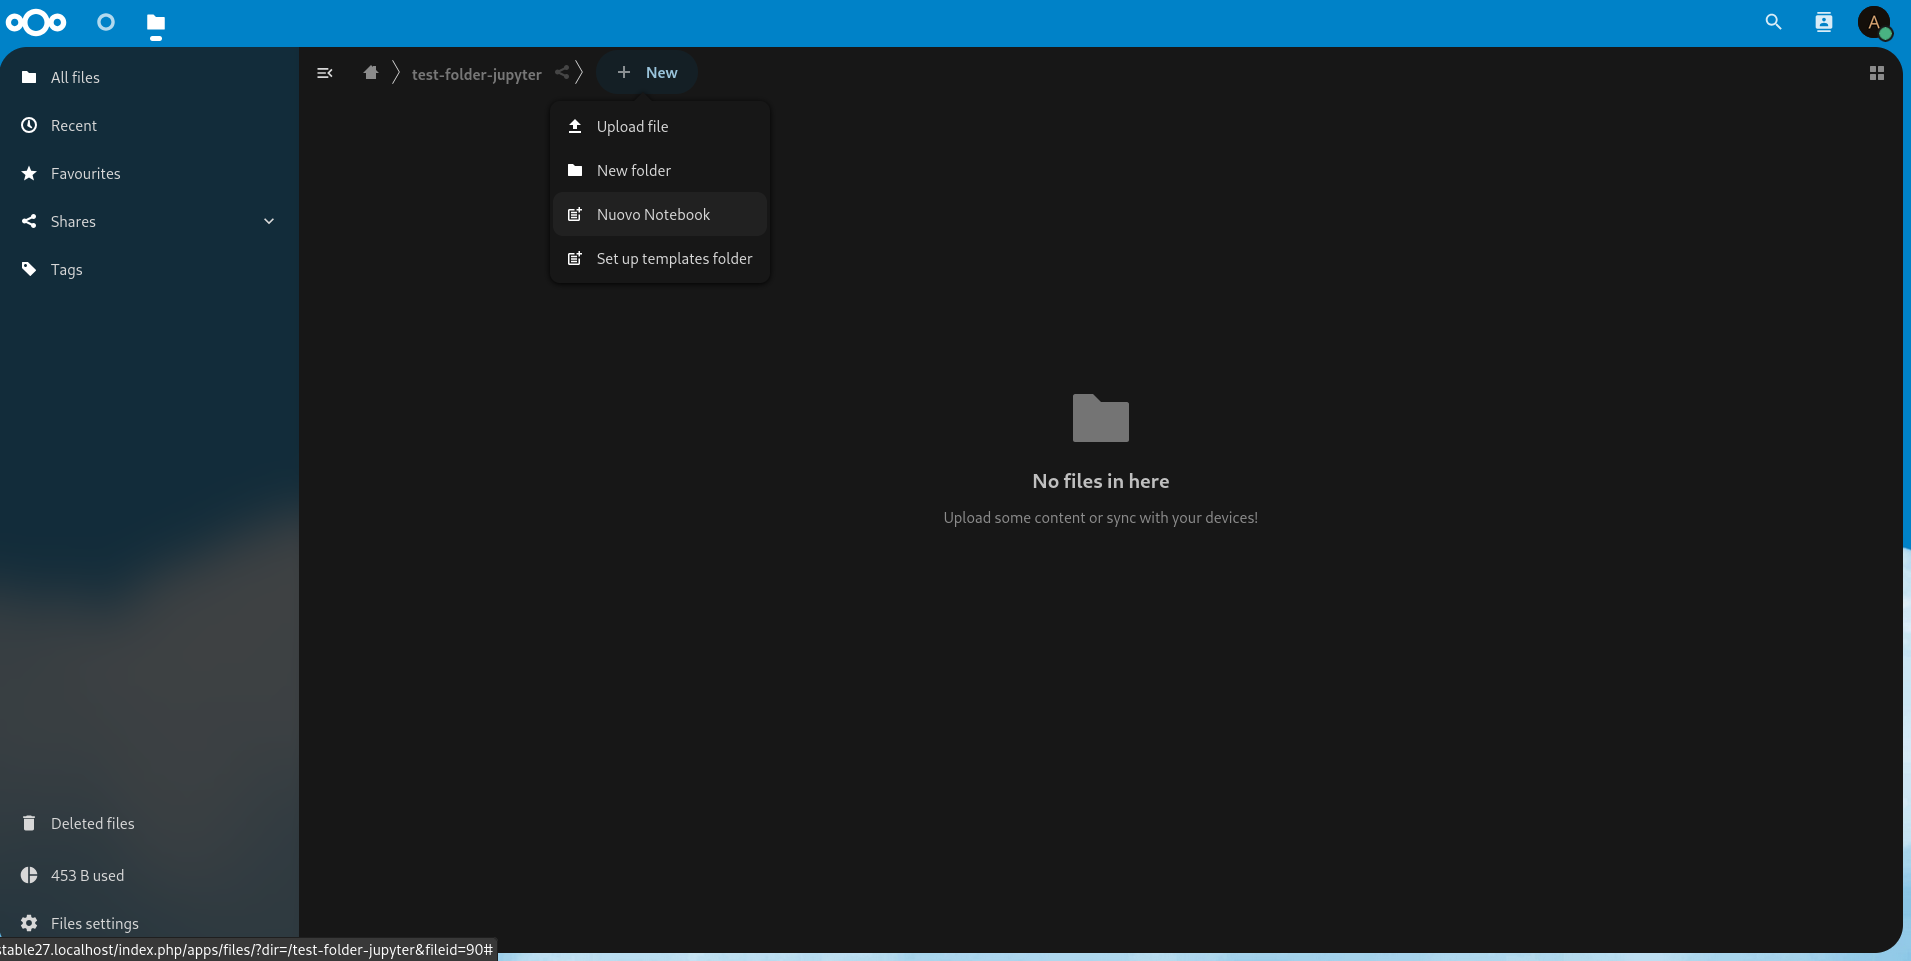
\includegraphics[width=1\textwidth]{files/images/example-nextpyter-1-2.png}
    \caption{Interfaccia grafica NextPyter "1.0" - Creazione notebook dentro la cartella}
    \label{fig:1.0-example-2}
\end{figure}
\begin{figure}[h]
    \centering
    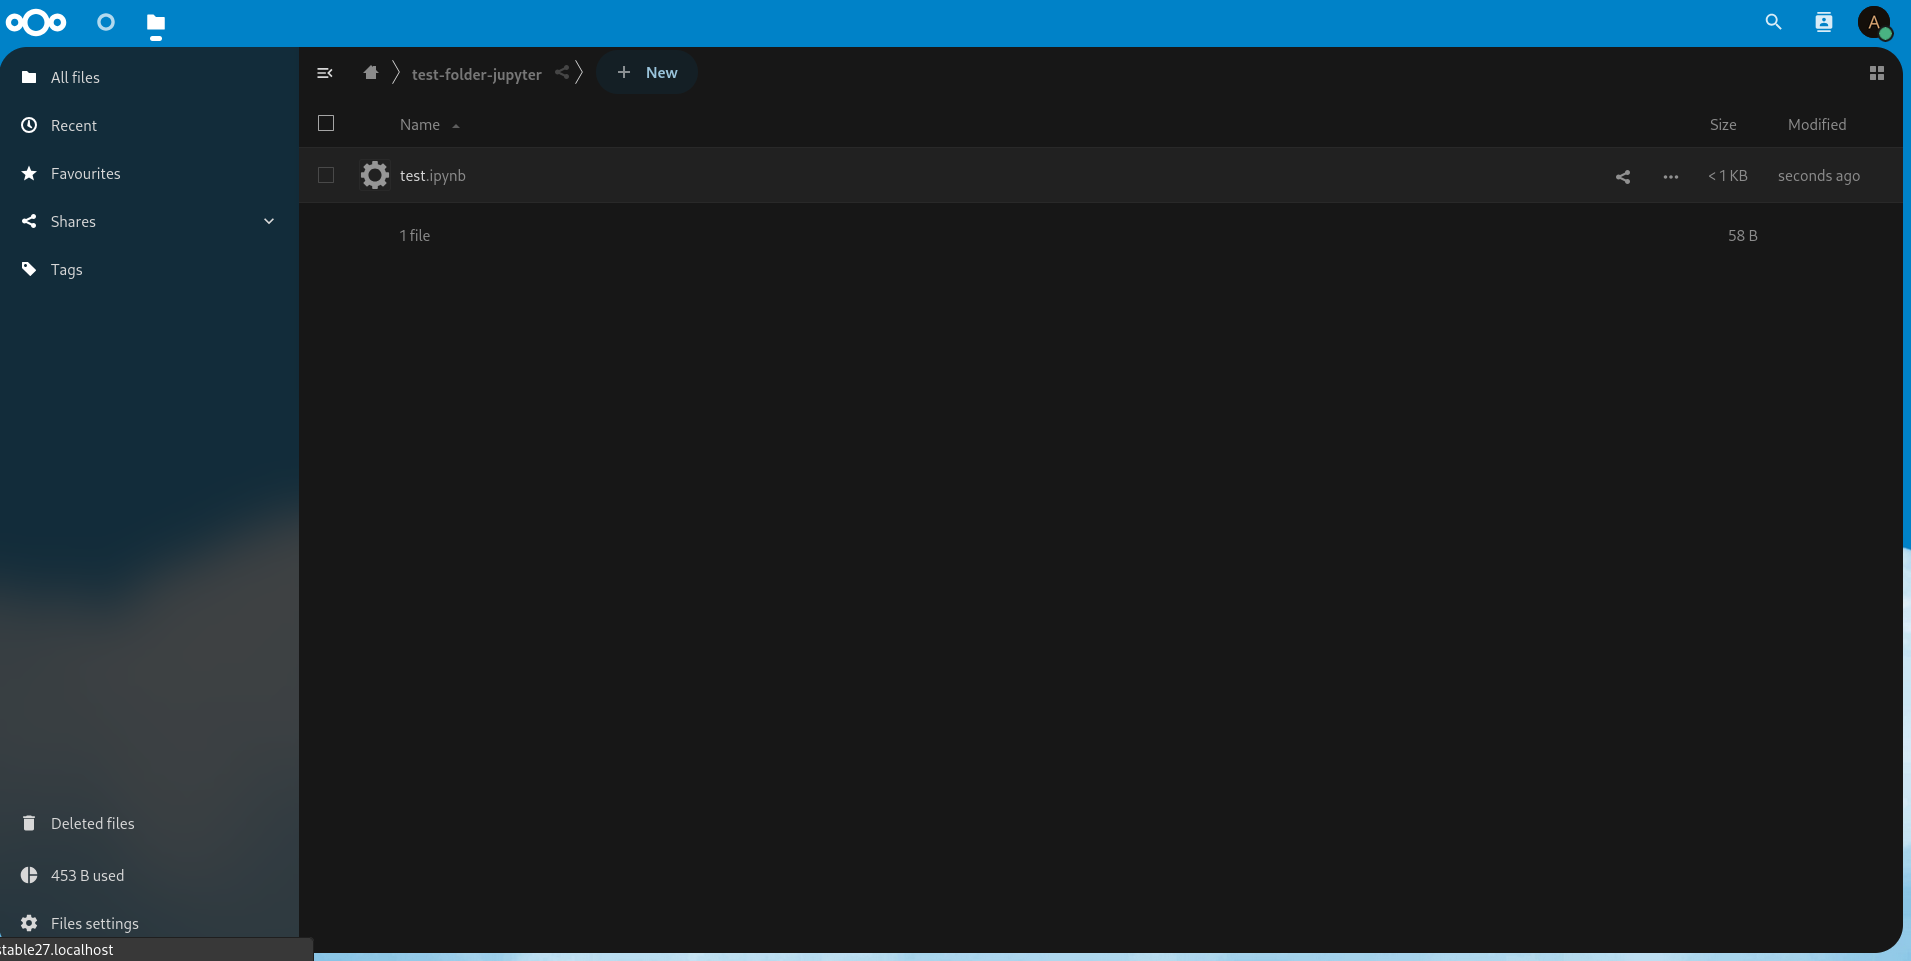
\includegraphics[width=1\textwidth]{files/images/example-nextpyter-1-3.png}
    \caption{Interfaccia grafica NextPyter "1.0" - Notebook creato}
    \label{fig:1.0-example-2}
\end{figure}
\begin{figure}[h]
    \centering
    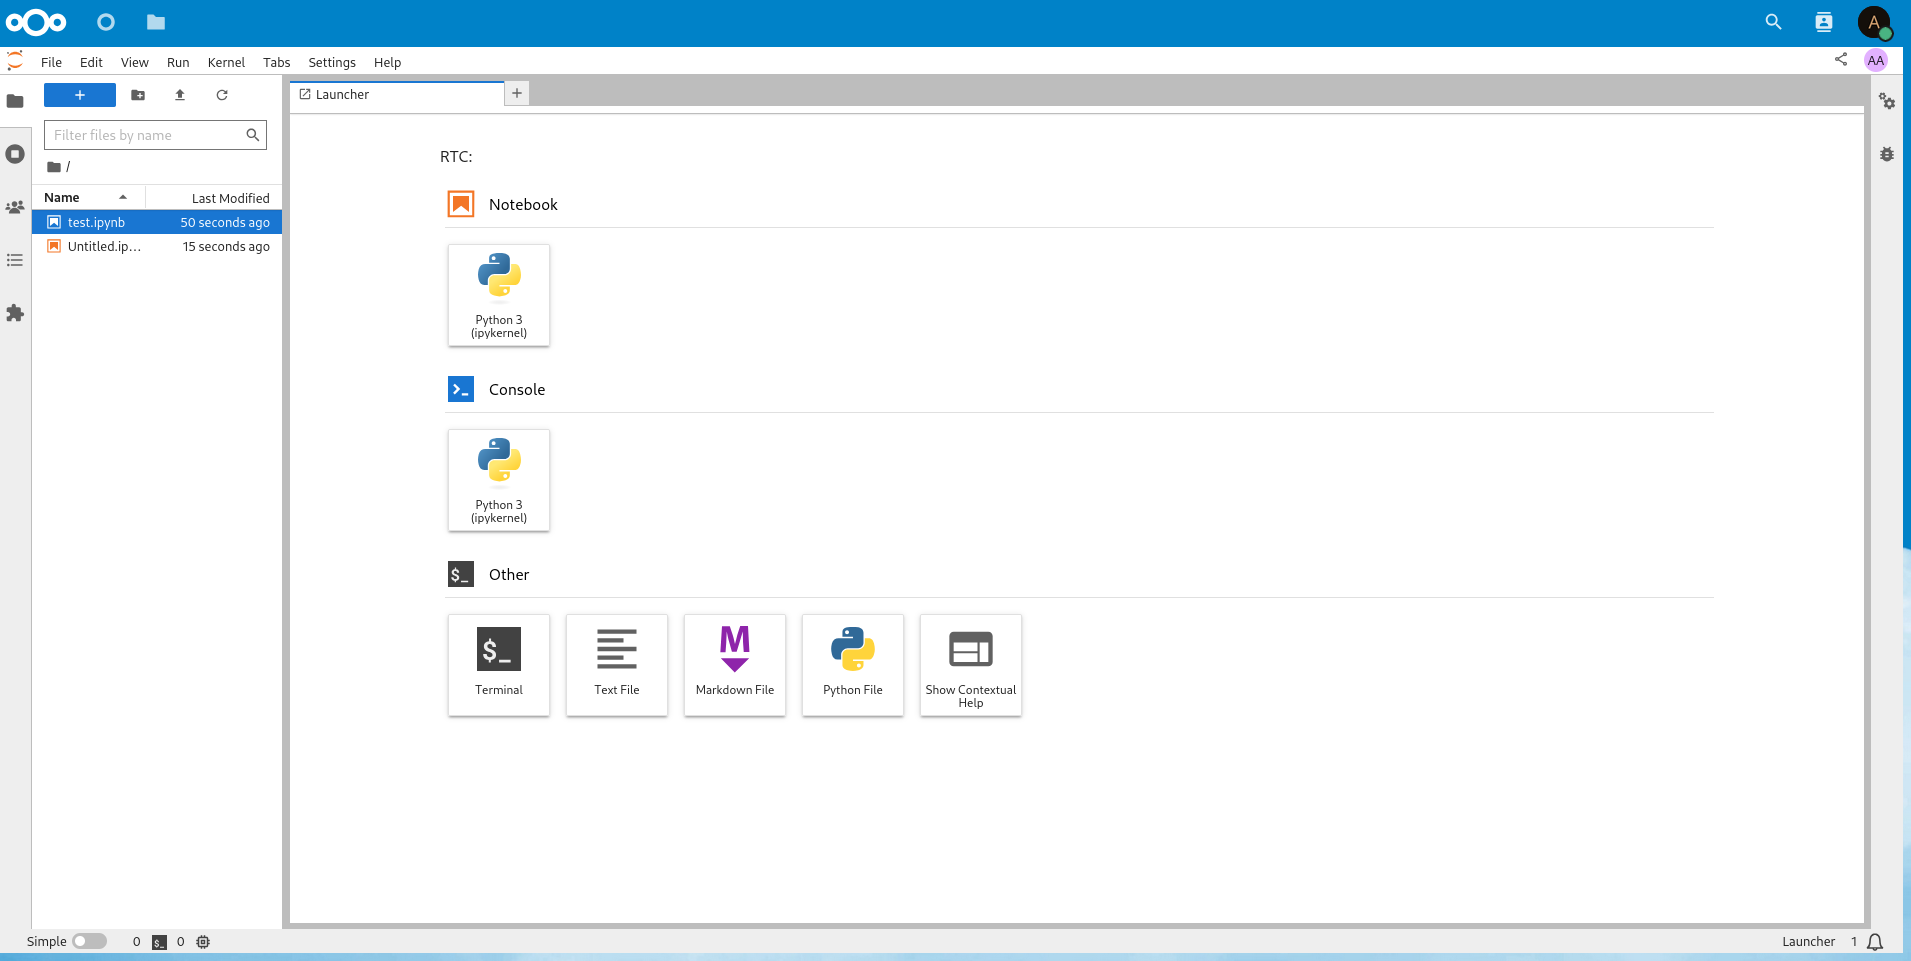
\includegraphics[width=1\textwidth]{files/images/example-nextpyter-1-4.png}
    \caption{Interfaccia grafica NextPyter "1.0" - Avviamento notebook}
    \label{fig:1.0-example-2}
\end{figure}

\subsubsection{Interfacciamento con Docker tramite Docker in Docker (DinD)}
Prima di spiegare effettivamente cosa sia Docker in Docker e come \textit{NextPyter} si interfaccia ad esso, è opportuno capire come Docker esponga le proprie funzionalità a client esterni, tra i quali, fra l'altro, figura il client a linea di comando di Docker stesso.
\newline
Docker è estensibile nel senso che è possibile sfruttare una API HTTP\footnote{https://docs.docker.com/reference/api/engine/}, esposta tramite un socket locale, per poter gestire programmaticamente \textit{container} all'interno dell'host in questione.
\newline
Ad esempio, è possibile interagire in maniera molto semplice con il \textit{daemon} di Docker tramite una semplice chiamata HTTP effettuata, in questo caso, con \textit{cURL}\footnote{https://curl.se/}.
\newline
Supponiamo di eseguire un container con \textit{NGINX} all'interno, usando il comando:
\begin{verbatim}
    docker run --rm -d nginx
\end{verbatim}
A questo punto, è possibile interrogare la REST API di Docker tramite una semplice chiamata \textit{GET} ad un URL specifico:
\begin{verbatim}
    curl --unix-socket /var/run/docker.sock http://localhost/containers/json
    [
    {
        "Id": "61969199e57ac0e1147e6092b110b895c47bc7913734f978377d53c428518107",
        "Names": [
            "/amazing_ride"
        ],
        "Image": "nginx",
        "ImageID": "sha256:8dd77ef2d82eade8...",
        "Command": "/docker-entrypoint.sh nginx -g 'daemon off;'",
        "Created": 1724752281,
        "Ports": [
            {
                "PrivatePort": 80,
                "Type": "tcp"
            }
        ],
        "Labels": {
            "maintainer": "NGINX Docker Maintainers"
        },
        "State": "running",
        "Status": "Up 4 seconds",
        "HostConfig": {
            "NetworkMode": "bridge"
        },
        "NetworkSettings": {
            "Networks": {
                "bridge": {
                    "IPAMConfig": null,
                    "Links": null,
                    "Aliases": null,
                    "MacAddress": "02:42:ac:11:00:02",
                    "NetworkID": "4a20cc24e78576fcd7c04b34a5208...",
                    "EndpointID": "048c2839a30529d26a6635c4af1d43...",
                    "Gateway": "172.17.0.1",
                    "IPAddress": "172.17.0.2",
                    "IPPrefixLen": 16,
                    "IPv6Gateway": "",
                    "GlobalIPv6Address": "",
                    "GlobalIPv6PrefixLen": 0,
                    "DriverOpts": null,
                    "DNSNames": null
                }
            }
        },
        "Mounts": []
    }
]
\end{verbatim}
\newpage
È possibile, ovviamente, eseguire anche un container tramite chiamate HTTP, sempre utilizzando l'API apposita:
\begin{verbatim}
    $ curl --unix-socket /var/run/docker.sock \
        -H "Content-Type: application/json" \
        -d '{"Image": "nginx", "Name": "esempio-nginx"}' \
       -X POST http://localhost/containers/create
    output: {
        "Id": "cf109023d2",
        "Warnings":[]
    }
    $ curl --unix-socket /var/run/docker.sock 
        -X POST http://localhost/v1.46/containers/cf109023d2/start
\end{verbatim}

Ovviamente, usando la chiamata vista in precedenza, si potrà vedere che il container è stato avviato con successo.
\newline
NextPyter fa pesante affidamento, ovviamente, sull'API offerta da Docker, poiché deve programmaticamente gestire il ciclo di vita di container, in base agli eventi che accadono sull'interfaccia utente di Nextcloud. Per fare ciò, la versione \textit{"1.0"} di NextPyter fa uso di due meccanismi principali che abilitano l'interfacciamento con Docker in maniera semplice: un'interfaccia software, DockerClient.php\footnote{https://gitlab.com/frfaenza/NextPyter/-/blob/main/lib/Service/DockerClient.php} e l'utilizzo di una procedura che comunemente viene chiamata \textit{Docker in Docker (DinD)}.
\newline
\textit{DinD} è necessario, poiché, generalmente, l'API HTTP del daemon è disponibile a livello di \textit{host}, quindi solo applicativi che risiedono su di esso (non containerizzati) possono, teoricamente, accedervi. Per aggirare questo limite, è possibile mappare il socket di Docker all'interno dei \textit{container} che ne dovranno fare uso uso, in questo caso quello di \textit{Nextcloud} (al quale accederà l'applicativo NextPyter).
\newline
Utilizzando, ad esempio, Docker Compose è possibile realizzare \textit{DinD} in maniera molto semplice:
\begin{verbatim}
    services:
        ubuntu:
            image: ubuntu
            volumes:
                - /var/run/docker.sock:/var/run/docker.sock:ro
\end{verbatim}
In questo modo si è creato un container basato su \textit{Ubuntu} che ha, montato, il file corrispondente al socket di Docker sull'host: notare come il \textit{mount} venga fatto \textit{read-only}; questo non significa che il socket non sarà scrivibile, ma che il \textit{file} mappato all'interno del container non lo sia. In questo modo si impedisce ad agenti interni al container di \textit{cancellare} il file corrispondente al socket, perché tutti i file \textit{mappati} all'interno di un container, se cancellati, lo saranno anche sull'host.
\newline
A questo punto sarà tranquillamente possibile eseguire i comandi precedentemente visti senza alcun problema, interagendo con Docker \textit{all'interno} di un container.

\newpage

\subsection{Criticità}
A seguito verranno elencate le criticità rilevate nel modello esposto dalla versione \textit{"1.0"}, sostanzialmente il motivo per il quale questa tesi esiste.

\subsubsection{Possibili vulnerabilità dovute a \textit{Docker in Docker}} \label{dind-acceptable}
Sebbene funzionale, l'approccio \textit{Docker in Docker} è generalmente riconosciuto \textit{potenzialmente pericoloso} \cite{dind}, per via del fatto che è possibile, sfruttando eventuali vulnerabilità di applicazioni containerizzate, accedere al socket Docker avendo, di fatto, completo controllo sul \textit{daemon} della macchina host.
\newline
Questa cosa è particolarmente preoccupante se si pensa che \textit{Nextcloud} non è un software che \textbf{nasce} con la pretesa di controllare un ambiente containerizzato, anzi, tutt'altro! Se, per caso, venisse introdotta una vulnerabilità che permette di eseguire codice arbitrario tramite una richiesta HTTP verso un'istanza \textit{Nextcloud} containerizzata, nulla vieterebbe l'attaccante di eseguire una richiesta al socket Docker riproducendo una richiesta simile a quelle viste in precedenza!
\newline
Il problema non è tanto \textit{DinD}, quanto il fatto che il \textbf{software} che ha accesso al socket, in questo caso \textit{Nextcloud}, non sia \textit{adibito specificatamente} alla gestione di questo approccio. 
\newline
In altre parole, \textit{DinD} è accettabile quando, nel container, è presente un software che ha come unico scopo quello di gestire il socket Docker, magari soddisfando richieste derivanti da altri container, in modo da essere l'unico punto di collegamento a Docker nel sistema containerizzato.
\begin{figure}[h]
    \centering
    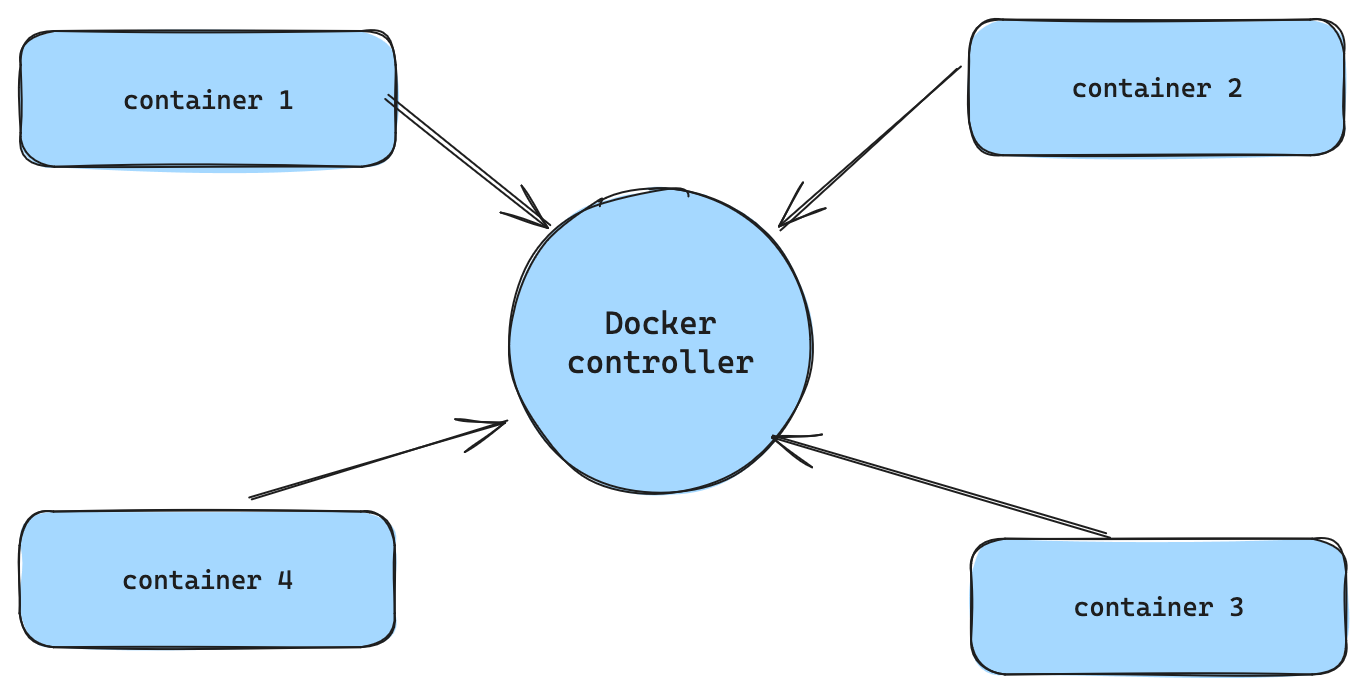
\includegraphics[width=0.75\textwidth]{files/images/dind-solution.png}
    \caption{Schematizzazione architettura accettabile per Docker in Docker}
    \label{fig:dind-acceptable}
\end{figure}
\newline
In figura \ref{fig:dind-acceptable}, infatti, è schematizzata un'architettura \textit{proposta come accettabile} per la gestione di questo approccio. Supponendo, ad esempio, che il \textit{Docker controller} esponga, a sua volta, un'API HTTP che mima quella di Docker (magari limitando l'accesso soltanto a determinati metodi), i container che vogliono consultare l'orchestratore lo potranno fare attraverso il \textit{Docker controller}, sfruttando l'API "limitata" che quest'ultimo offre. Nel corso del documento verrà descritto in più dettaglio questo "nuovo" approccio.
\newpage
\subsubsection{Gestione delle risorse di rete dei notebook} \label{net-acceptable}
Allo stadio attuale, le porte TCP dei container vengono mappate direttamente sull'host che gestisce l'orchestratore. Questa pratica, oltre ad imporre un limite massimo al numero di notebook che si possono mappare sull'interfaccia di rete dell'host, è particolarmente macchinosa da un punto di vista applicativo, dato che è necessario \textbf{scansionare} l'host alla ricerca di porte aperte.
\newline
Una soluzione al problema può essere quella di posizionare "di fronte" ai container un componente che si occupa dell'instradamento del traffico a questi ultimi facendo leva sui meccanismi di \textit{networking} interni a Docker, come visibile in figura \ref{fig:routing}
\begin{figure}[h]
    \centering
    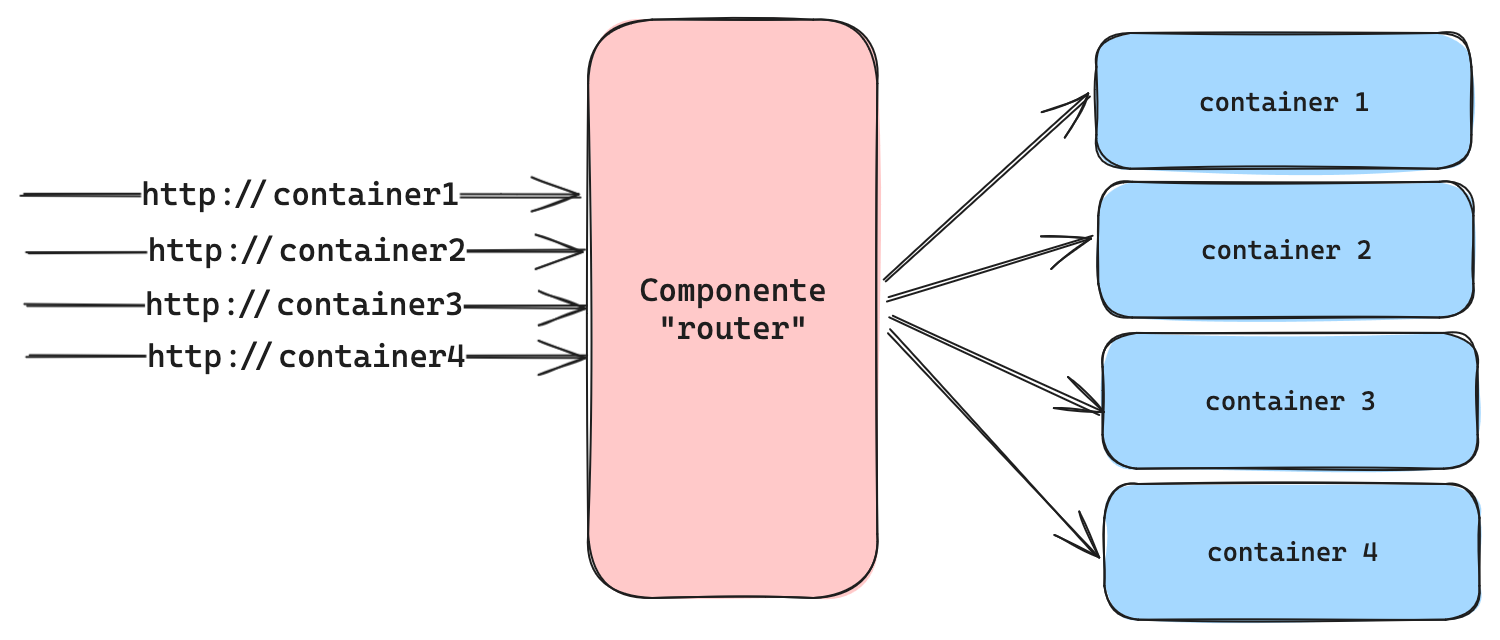
\includegraphics[width=1\textwidth]{files/images/routing-solution.png}
    \caption{Routing traffico verso container}
    \label{fig:routing}
\end{figure}
\newline
In questa maniera, l'unica porta esposta sull'host è quella sul componente "router", alla quale le richieste esterne potranno essere mandate, mentre sarà compito di quest'ultimo quello di instradare correttamente il traffico verso le porte interne, non esposte, dei vari container.
\subsubsection{Mancanza supporto per la gestione delle immagini Docker}
Allo stato attuale, la gestione delle immagini Docker per i vari notebook non è supportata. Uno dei requisiti dell'attività che ha portato a questa tesi è quello di creare un supporto al download e alla configurazione delle immagini che possono essere utilizzate per avviare i notebook, pertanto è stato sviluppato un componente \textit{ad-hoc} che verrà commentato successivamente.

\newpage
\section{NextPyter \textit{"2.0"}}
Analizzate le criticità del progetto nella versione \textit{"1.0"}, la sua architettura e le eventuali migliorie applicabili, il tema centrale di questa tesi sarà la descrizione del processo di progetto e sviluppo della versione \textit{"2.0"} della piattaforma, creata appositamente per apportare i cambiamenti richiesti, aggiungendo anche il supporto all'orchestratore di container \textit{Kubernetes}.
\newline
\begin{figure}[h]
    \centering
    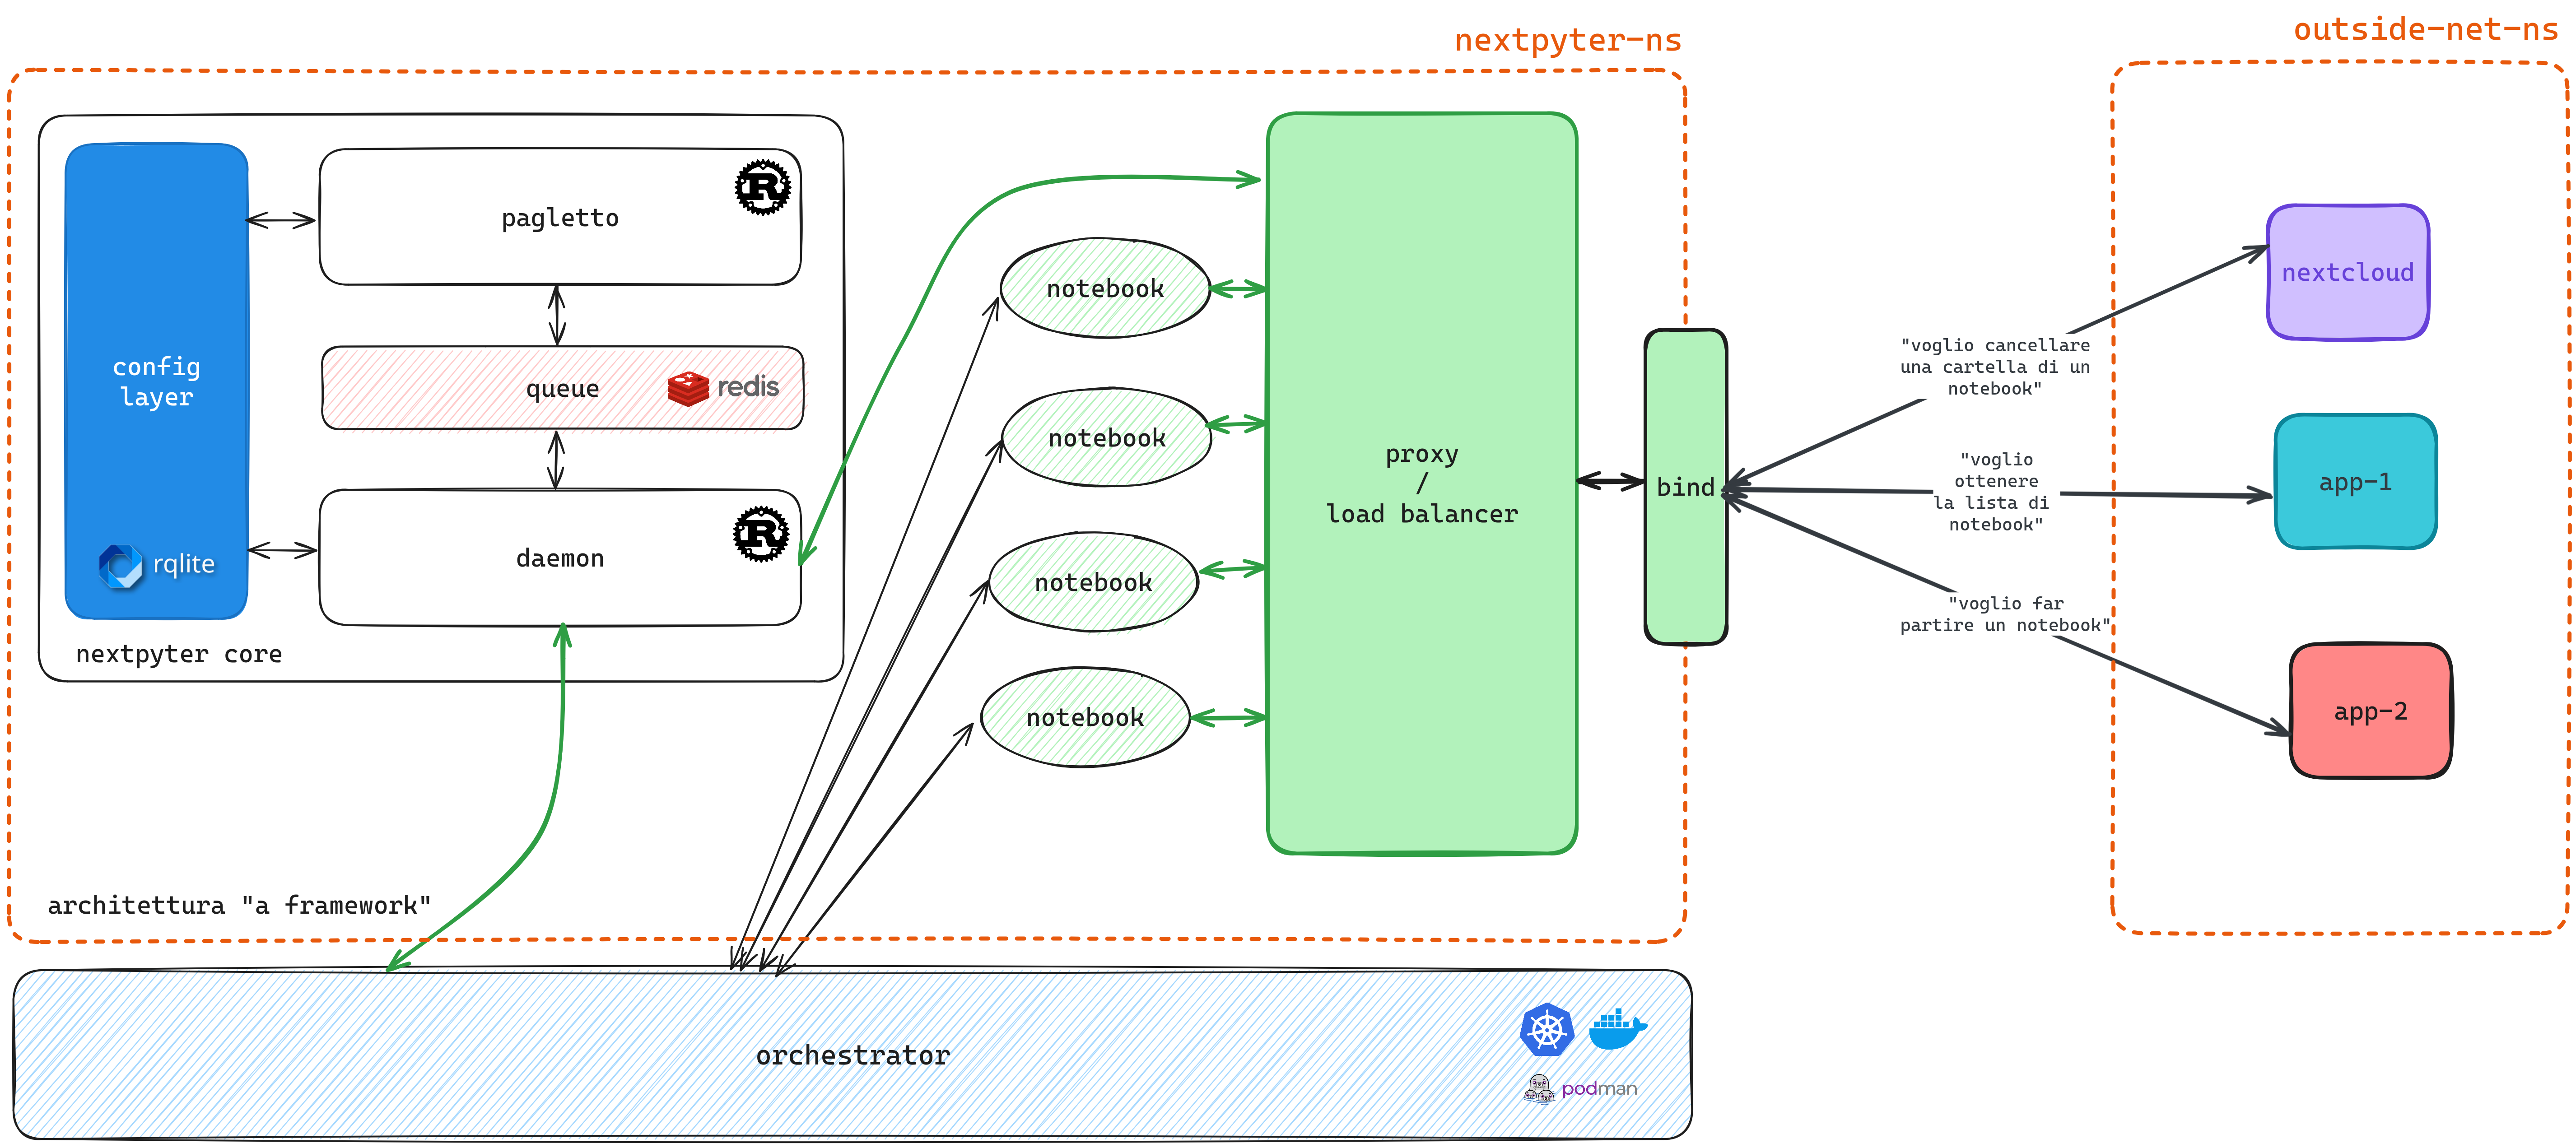
\includegraphics[width=1\textwidth]{files/images/nextpyter-2-diagram.png}
    \caption{Schema architetturale NextPyter \textit{"2.0"}}
    \label{fig:nextpyter-2-diagram}
\end{figure}
\newline
Sono stati identificati i seguenti nuovi obiettivi per NextPyter \textit{"2.0"}:
\begin{itemize}
    \item Supporto a Kubernetes: questo requisito non è stato esattamente identificato, semplicemente era il \textit{titolo dell'attività tirocinio}, pertanto è l'obiettivo "di arrivo" di questa tesi;
    \item Supporto alla \textit{high availability}: è stato individuato il bisogno di voler espandere la piattaforma ad una platea di utenti molto più grande. Da piattaforma installabile tramite Docker e Docker Compose, NextPyter dovrà trasformarsi in un'altra in grado di scalare orizzontalmente in modo da garantire il corretto soddisfacimento di più classi di traffico. Pertanto, non solo sarà necessario supportare Kubernetes, ma tutti i componenti che realizzano NextPyter, che analizzeremo successivamente, dovranno essere in grado di mostrare un determinato grado di \textit{resilienza}. In altre parole, NextPyter \textit{"2.0"} dovrà supportare egregiamente una quantità di traffico modellabile come le richieste provenienti da gruppi di ricerca di più dipartimenti dell'Università di Modena e Reggio Emilia, a grandi linee (eventualmente scalando oltre!);
    \item Miglioramento del supporto a Docker: nonostante la richiesta dell'implementazione del supporto a Kubernetes, è stato deciso di mantenere il supporto a Docker per supportare scenari più piccoli;
    \item Configurazione dinamica: allo stato attuale, la versione \textit{"1.0"} non prevede la configurazione dinamica delle immagini per i container dei notebook. La piattaforma \textit{"2.0"} dovrà essere in grado di supportare questo genere di requisito;
    \item Autorizzazione \textit{fine-grained} delle richieste: i componenti che vorranno interfacciarsi con NextPyter lo potranno fare mediante un set di permessi che verrà definito in un \textit{layer} di autenticazione che regolerà l'accesso al sistema in maniera estremamente granulare, usando un meccanismo che permetta di filtrare le richieste basandosi, virtualmente, su qualsiasi aspetto di quest'ultima;
\end{itemize}
\newline
In figura \ref{fig:nextpyter-2-diagram} è raffigurato un diagramma che illustra, ad alto livello, i nuovi componenti della piattaforma, che verranno approfonditi in dettaglio nei paragrafi a venire.
\newline
\subsection{NextPyter come \textit{framework}}
Una delle prime, se non la prima, necessità del progetto è stata sicuramente quella della creazione di un componente che scorporasse le funzionalità base di NextPyter da \textit{Nextcloud}: la complessità e profondità dei requisiti succitati non può fare affidamento su un componente del genere, perché troppo dipendente sulla presenza di un altro software. Le logiche che derivano, ad esempio, dal requisito riguardante la \textit{high availability} richiedono che ciascun componente del sistema scali indipendentemente rispetto agli altri, per riuscire a gestire volumi di traffico variabili: nella piattaforma \textit{"1.0"}, l'applicazione NextPyter non può scalare indipendentemente, poiché è strettamente vincolata all'ambiente in cui viene eseguita, ovvero \textit{Nextcloud} stesso.
\newline
L'idea fondamentale, quindi, è quella della realizzazione di un'entità a sé, con un perimetro ben definito all'interno del sistema: il cosiddetto \textit{core} di NextPyter.
\newline
La progettazione della nuova piattaforma ha visto la necessità di rendere le funzionalità base di NextPyter, la gestione di notebook Jupyter, quindi, un \textit{framework} accessibile tramite HTTP(S) dai più svariati client che vogliano implementarlo. In questo modo, NextPyter non è più legato necessariamente ad un'installazione di \textit{Nextcloud}, ma è estensibile da qualsiasi client voglia implementare le sue funzionalità, tramite interfacce che verranno descritte in maggior dettaglio fra qualche paragrafo.
\subsubsection{Controllo dei container: il modulo \textit{daemon}}
Il modulo di "rappresentanza" del \textit{core} di NextPyter è sicuramente il \textit{daemon}, poiché esporrà l'API HTTP che permetterà di poter interagire con le logiche di NextPyter.
\newline
Questo modulo dovrà essere realizzato tenendo a mente i seguenti principi:
\begin{itemize}
    \item Riduzione della \textit{attack surface} derivante dall'approccio \textit{DinD}: dal momento in cui NextPyter dovrà comunque supportare Docker, è stato necessario revisionare l'approccio all'interazione col \textit{Docker daemon}. In particolare, l'unico componente che avrà accesso al socket di Docker sarà il \textit{daemon} di NextPyter e tutti gli altri componenti del sistema, ogniqualvolta vorranno fare operazioni riguardanti la gestione dei notebook, dovranno riferirsi al \textit{daemon} stesso. L'approccio è il medesimo descritto nel paragrafo \ref{dind-acceptable};
    \item Least privilege: i client che vorranno interfacciarsi a \textit{daemon} lo faranno utilizzando un set di richieste specifiche che verranno filtrate appositamente dal layer di autenticazione e autorizzazione descritto in precedenza. In questo modo, tramite un set di regole ben definite, client diversi potranno accedere in maniere diverse e completamente personalizzabili al sistema;
    \item Isolamento delle risorse: come già ancitipato, qualsiasi componente del \textit{core} dovrà essere in grado di scalare orizzontalmente (e verticalmente, volendo);
    \item Minimizzazione delle dipendenze: NextPyter deve essere progettato in modo da ridurre non solo le dipendenze di traffico, ma anche quelle di codice. A questo pro, per l'appunto, è stata sviluppata l'interfaccia HTTP di cui sopra, per realizzare un protocollo implementabile da qualsiasi client;
    \item Astrazione dell'orchestratore di \textit{container}: poiché la piattaforma dovrà supportare sia Docker che Kubernetes, sarà necessario sviluppare l'API REST in una maniera che prescinde completamente dal tipo di orchestratore con la quale il modulo andrà a comunicare. I client che si interfacceranno con \textit{daemon} non avranno la necessità di sapere se quest'ultimo sia in collegamento con Kubernetes o con Docker: tutto sarà completamente trasparente agli utilizzatori e l'interfaccia sarà la medesima in entrambi i casi, semplificando nettamente lo sviluppo dei client.
\end{itemize}
\subsubsection{Configurazione dinamica: il modulo \textit{pagletto}, \textit{RQLite} e \textit{Valkey}}
Questo modulo, dal nome che non significa particolarmente nulla, accoppiato ad un database ad alta disponibilità, \textit{RQLite} e \textit{Valkey}, un database \textit{key-value}, soddisferà il requisito di configurazione dinamica delle immagini. In particolare, come visibile anche dallo schema, sarà possibile, mediante una chiamata API HTTP fatta verso \textit{daemon}, richiedere il download di un'immagine \textit{Docker} dal \textit{registry} ufficiale (configurabile, eventualmente). Questa immagine, una volta scaricata, verrà registrata nel database \textit{RQLite}\footnote{https://rqlite.io/}, un \textit{fork} di \textit{SQLite} progettato per essere leggero e \textit{highly available}.\newline
Infatti, RQLite è un database SQL che è in grado di replicare i dati per questioni di \textit{fault tolerance}, rendendoli disponibili tra più nodi, in modo che se uno di questi è soggetto a malfunzionamenti, l'accesso sia comunque garantito dai rimanenti. Oltre a questo, RQLite funziona mediante un protocollo a elezione di \textit{leader}, \textbf{\textit{raft}}\footnote{https://raft.github.io/}, pertanto vi saranno copie autoritative e copie non autoritative dei dati, in modo da garantire che lo stato del database sia sempre integro. Questo tipo di database è stato scelto perché è implementato in maniera estremamente semplice, astraendo tutte le chiamate di basso livello attraverso, anche qui, una API REST.
A questo punto, gli unici container avviabili, sempre tramite un'apposita chiamata HTTP, saranno quelli che avranno immagini che compaiono all'interno della configurazione distribuita, rendendo più sicura l'interazione con l'orchestratore da parte di \textit{daemon}.
\newline
Per realizzare la comunicazione tra \textit{daemon} e \textit{pagletto} sarà utilizzato \textit{Valkey}, un database \textit{key-value}, il \textit{fork open source} del progetto \textit{Redis}\footnote{https://www.linuxfoundation.org/press/linux-foundation-launches-open-source-valkey-community}, sfruttando la tecnologia di \textit{event streaming} fornita da Valkey stesso, che verrà dettagliata nei prossimi paragrafi. 

\subsubsection{Utilizzo di NGINX per ottimizzare la gestione delle risorse di rete: il modulo \textit{proxy}}
Come già anticipato in sezione \ref{net-acceptable}, la versione \textit{"1.0"} di NextPyter gestiva le risorse di rete in maniera subottimale. Per sopperire a questo problema, è stato deciso di implementare il \textit{routing} del traffico di tutto il \textit{core} mediante l'utilizzo di \textit{NGINX} configurato come \textit{reverse proxy}.
\newline
Un reverse proxy è un componente di rete che si interpone tra la comunicazione fra client e server, in questo caso i \textit{notebook}, principalmente, con lo scopo di gestire e regolare le richieste in entrata al sistema, eventualmente modificandole o validandole mediante un qualche genere di logica (anche personalizzata).
\newline
NGINX, nell'ecosistema NextPyter, viene usato proprio a questo scopo: viene interposto fra la comunicazione con l'esterno e i notebook, in modo da fornire una serie di garanzie che senza di esso sarebbe difficile fornire, come ad esempio la verifica dell'autenticità delle richieste, il bilanciamento delle richieste in arrivo e, tra le altre cose, il "mascheramento" delle porte dei notebook verso l'esterno. La configurazione di NGINX, infatti, è sostanzialmente la stessa che viene proposta nella sezione \ref{net-acceptable}, che verrà dettagliata maggiormente nel prossimo capitolo, dove verrà descritta l'implementazione dell'architettura di NextPyter \textit{"2.0"}.
\newline
Oltre a questo, NGINX verrà utilizzato per via della sua ampia estensibilità: infatti, oltre ad essere un \textit{load balancer}, NGINX è configurabile per essere \textit{application gateway}, ovvero un componente che è in grado di trascendere dal classico ruolo di bilanciatore del traffico e implementare l'indirizzamento delle richieste basandosi su logiche completamente personalizzate.
\newline
Questo obiettivo verrà realizzato mediante \textit{NJS}, sostanzialmente un motore JavaScript progettato per l'utilizzo all'interno di NGINX. Creato per estendere le capacità di scripting del server NGINX, \textit{NJS} consente di manipolare le richieste HTTP e le risposte in tempo reale, facilitando la gestione avanzata delle richieste, la modifica delle intestazioni, il controllo degli accessi, il routing dinamico e altre personalizzazioni senza compromettere le prestazioni. Questo linguaggio è integrato direttamente in NGINX, consentendo l'esecuzione di script lato server in modo efficiente e sicuro, con un impatto minimo sulle prestazioni del server web.
\subsubsection{Documentazione autogenerate: il modulo \textit{docs}}
Per via della natura dell'ecosistema di NextPyter \textit{"2.0"}, è stato ritenuto opportuno includere un modulo che permettesse la consultazione della documentazione dell'API HTTP fornita dal modulo \textit{daemon} in maniera semplice e \textit{user-friendly}.
\newline
A questo scopo, sfruttando lo standard OpenAPI, verrà messo a punto un sistema per il quale, una volta che \textit{daemon} verrà compilato, sarà creato un \textit{endpoint} HTTP che espone la documentazione riguardante la API REST seguendo lo standard \textit{openapi 3.0}. Una volta esposto l'endpoint, verrà messo a punto un altro modulo, \textit{docs}, che interperllerà tale endpoint di documentazione, effettuerà operazioni di \textit{parsing} e lo presenterà tramite un'interfaccia \textit{user friendly}. Questo modulo sarà reso disponibile utilizzando \textit{Swagger UI}\footnote{https://swagger.io/tools/swagger-ui/}, uno strumento open-source utilizzato per visualizzare e interagire con le API web che seguono la specifica OpenAPI (precedentemente nota come Swagger Specification). È un'interfaccia grafica che consente alle sviluppatrici e agli sviluppatori di esplorare, testare e documentare le API in modo interattivo.
\begin{figure}[h]
    \centering
    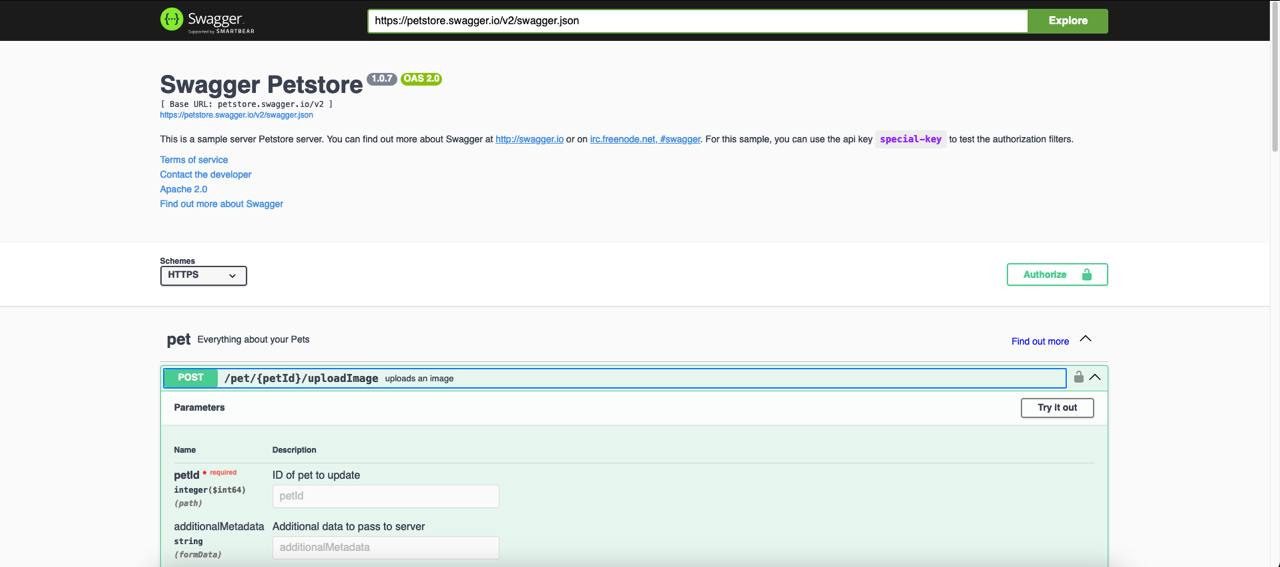
\includegraphics[width=1\textwidth]{files/images/swagger-ui.jpg}
    \caption{Interfaccia di Swagger UI}
    \label{fig:swagger-ui}
\end{figure}

\subsubsection{Sommario}
Nella progettazione di NextPyter \textit{"2.0"}, è stata posta particolare enfasi sulla modularità e l'indipendenza del sistema, elementi chiave per superare le limitazioni della versione 1.0. In quest'ultima, la piattaforma era strettamente vincolata a Nextcloud, il che limitava fortemente la capacità di scalare e adattarsi alle nuove esigenze. La nuova architettura si distacca radicalmente da questo modello, adottando un approccio modulare che separa chiaramente le varie funzionalità del sistema. Questo consente di gestire, aggiornare e migliorare ciascun componente in modo indipendente, riducendo le interdipendenze che complicano la manutenzione e l'evoluzione della piattaforma. Ciò permette al sistema di scalare orizzontalmente, gestendo efficacemente grandi volumi di traffico e garantendo alta disponibilità e resilienza, elementi fondamentali per supportare le richieste di gruppi di ricerca diversi e numerosi. Inoltre, l'indipendenza dei moduli consente alla piattaforma di evolversi più facilmente, integrando nuove tecnologie o migliorando quelle esistenti senza necessità di ristrutturazioni complesse o invasive. Questa flessibilità rappresenta un notevole passo avanti rispetto alla versione precedente, rendendo NextPyter 2.0 una piattaforma più robusta, adattabile e pronta per future sfide e opportunità di espansione.

\subsection{Progettazione layer di autenticazione}
Per mantenere le faccende quanto più modulari e indipendenti possibili, è stato scelto di rendere il \textit{layer} di autenticazione, almeno in questa fase iniziale della nuova piattaforma, un componente facoltativo, sottolineando un'altra volta la estrema modularità del sistema.
\newline
Nell'immagine \ref{fig:nextpyter-2-diagram}, si può notare come questo modulo sia presente, quando attivato, in tutte le interazioni che vengono fatte all'interno del sistema, per garantire, appunto, sicurezza e autenticità nelle transazioni.
\newline
Il tipo protocollo che si è deciso di supportare è \textit{OAuth2}, sostanzialmente lo standard \textit{de-facto} \cite{auth0} dell'industria per quanto riguarda autenticazione e autorizzazione tra microservizi.
\newline
\subsubsection{Cos'è OAuth2}
\textit{Premessa: questa sezione è stata tratta, tradotta e adattata da un progetto dell'autore della tesi \footnote{https://github.com/emilianomaccaferri/oauth2-spring-boot/blob/main/chapters/Chapter\%20I.md}}.
\newline
\newline
OAuth2 è uno \textit{standard}, un \textit{protocollo}, come già menzionato, non qualcosa che è possibile "eseguire", che permette di definire un set di operazioni che realizzano l'autenticazione e l'autorizzazione in un determinato sistema.\newline
Per poter utilizzare questo standard, dunque, è necessario utilizzare un cosiddetto \textit{identity provider}, o \textit{IDP}, che implementi \textit{OAuth2}, sostanzialmente un software che realizza ciò che viene definito nello standard.
\newline
Uno degli IDP di più rilievo è sicuramente Keycloak \cite{keycloak-stats}, sviluppato e mantenuto da \textit{RedHat}. Oltre a questo, Keycloak è completamente open source e utilizzabile come software \textit{self-hosted}, rendendolo la scelta perfetta per un sistema con i vincoli, anche di dipendenza da \textit{vendor} di servizi cloud, di NextPyter.

\subsubsection{OAuth2 in dettaglio}
Come si ottiene accesso ad un set di risorse protette da un IDP OAuth2? La risposta è semplice, mediante l'utilizzo di un \textbf{flow}, un insieme di "passi" che l'IDP metterà in atto per verificare l'identità di un client che vuole accedere al sistema.
\newline
I principali flow che verranno descritti in questa sezione sono l'\textit{authorization code flow} e il \textit{service account flow} (nota: i nomi di questi flow possono cambiare da IDP a IDP, in questa sezione sono stati usati i nomi più utilizzati nell'industria). 
\newline
Il primo è utilizzato quando il client che sta cercando di accedere alle risorse protette è un sito web o un'applicazione mobile, o comunque qualsiasi tipo di applicazione la cui interazione con il sistema è guidata da un utente, mentre il secondo tipo di flow viene utilizzato da applicazioni che non sono guidate da utenti, come servizi di automazione, servizi di logging, script esterni, microservizi e quant'altro.
\newline
Entrambi i flow, comunque, utilizzano due informazioni molto importanti, cruciali nella realizzazione di tutte logiche di autenticazione e autorizzazione: \textit{access token} e \textit{refresh token}.
\begin{itemize}
    \item Un \textit{access token} viene utilizzato per effettuare \textbf{richieste autenticate} al sistema. La caratteristica principale di questo tipo di token è che hanno una vita particolarmente breve, per via del fatto che questo genere di informazioni, ovvero quelle che permettono l'accesso diretto ad un sistema, sono soggette a \textbf{leak}, i protocolli di sicurezza vengono \textbf{penetrati}, insomma, tante cose possono andare male, pertanto ha senso \textit{agire in favore di sicurezza} e dare un \textit{TTL} basso a questo genere di token;
    \item Un \textit{refresh token}, invece, viene utilizzato per \textbf{ottenere nuovi \textit{access token}} quando questi scadono. Questi, a differenza degli altri, hanno un \textit{TTL} particolarmente lungo e, per questo motivo, vanno mantenuti con particolare scrupolo.
\end{itemize}
\newpage
\subsubsection{Funzionamento dell'\textit{authorization code flow}}
Per descrivere in maniera concisa il funzionamento di questo processo, verrà utilizzata come riferimento l'immagine \ref{fig:auth-code-flow} qui sotto.
\begin{figure}[h]
    \centering
    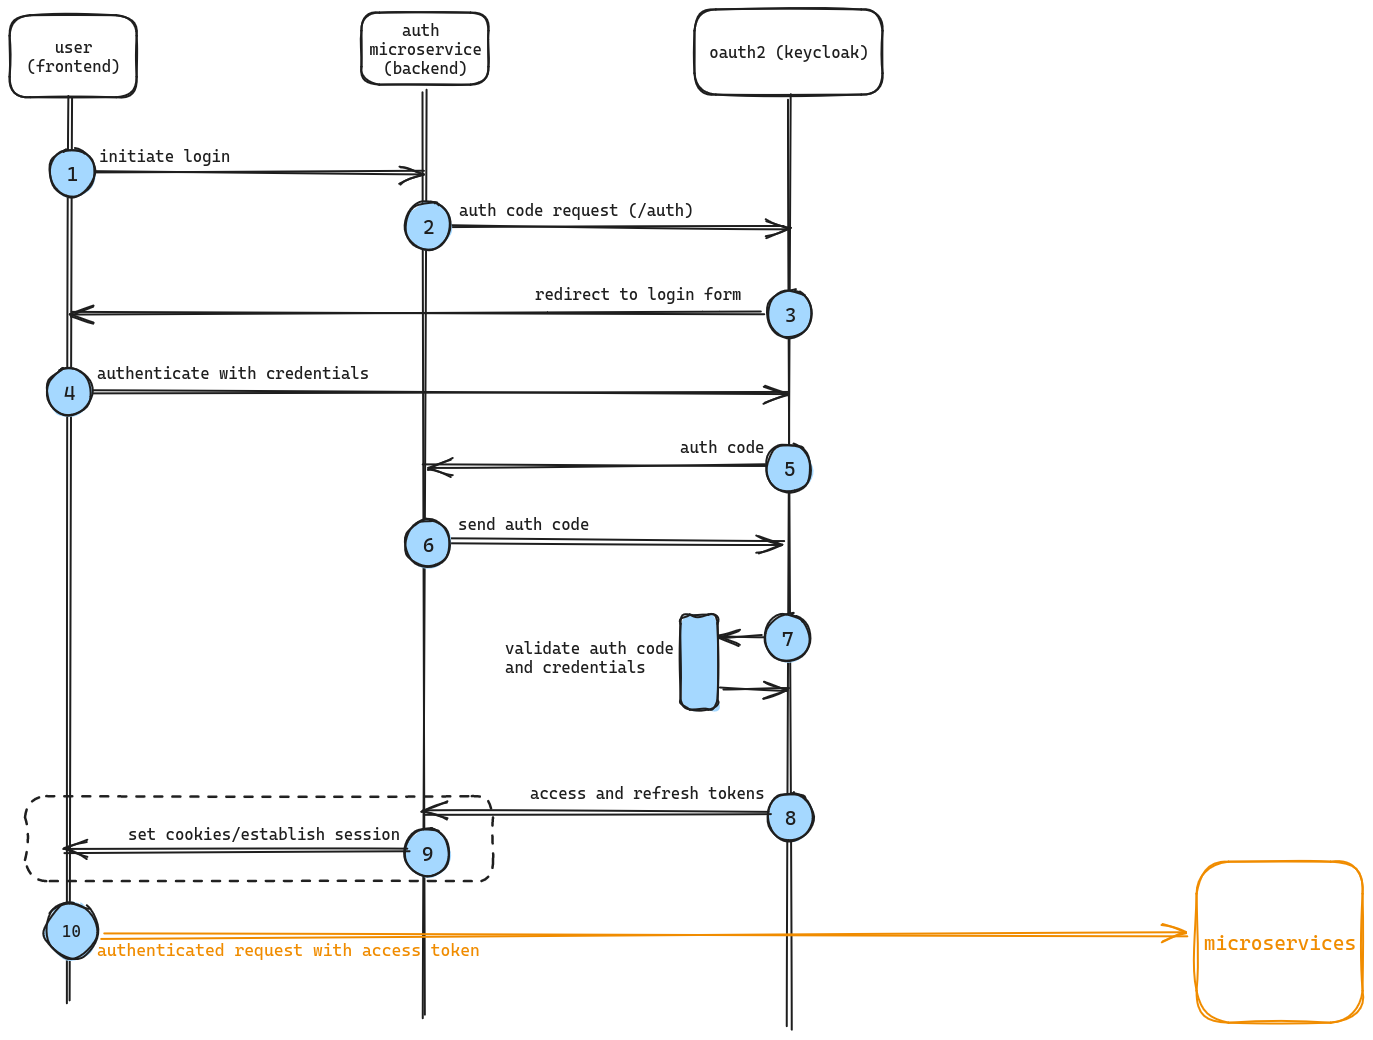
\includegraphics[width=1\textwidth]{files/images/auth-code-flow.png}
    \caption{Authorization code flow}
    \label{fig:auth-code-flow}
\end{figure}
\newline
Il flusso può essere dettagliato come segue:
\begin{itemize}
    \item L'utente clicca sul classico bottone di login;
    \item Il backend del sito web su cui viene effettuata la richiesta di login effettua una cosiddetta \textit{authorization code request}. Questa azione fa ridirigere l'utente al form di login (che può essere il classico \textit{"Login con Google"} o equivalenti);
    \item L'utente viene ridiretto al form di login;
    \item L'utente si autentica;
    \item Se le credenziali sono corrette, un \textit{auth code} è inviato al backend iniziale, quello del sito d'origine;
    \item Una volta che l'\textit{auth code} è stato ricevuto dal backend, questo effettua un'ulteriore richiesta per ottenere gli \textit{access} e \textit{refresh token}. Notare come la presenza di un \textit{auth code} sia critica per mitigare una serie di rischi di sicurezza non banali: emettendo un \textit{auth code}, il client di origine \textbf{non contatta mai direttamente l'\textit{IDP}} che regola l'accesso al sistema e il processo di autenticazione è completamente delegato a \textit{backend} e \textit{IDP}. Questa cosa rafforza particolarmente la sicurezza del processo e, in particolare, non permette accesso privilegiato \textbf{diretto} all'\textit{IDP} da parte di client potenzialmente vulnerabili. Se, ad esempio, il token non venisse passato direttamente al server, ma venisse passato ad un client vulnerabile, l'\textit{auth code} sarebbe rubato e l'intero flusso di autenticazione sarebbe corrotto, permettendo ad attaccanti esterni di autenticarsi come se fossero il client legittimo! Quello che accade, invece, è che il backend richiede le credenziali (i token di cui sopra) con l'\textit{auth code} e l'\textit{IDP} è configurato per ricevere richieste di autenticazione solo da tale servizio, rafforzando ancora di più la sicurezza del processo;
    \item L'IDP verifica le credenziali e l'\textit{auth code} presentato;
    \item I token vengono emessi e...
    \item ... una sessione di autenticazione viene creata tra frontend e backend;
    \item L'utente potrà fare, ora, richieste autenticate al sistema.
\end{itemize}
\newpage
\subsubsection{Funzionamento \textit{service account flow}}
Come già menzionato, i \textit{service account} sono tutte quelle applicazioni "autonome" e non guidate da utenti, come aggregatori di log, servizi di notifiche, ...\newline
In maniera del tutto analoga al caso precedente, verrà utilizzata l'immagine \ref{fig:sa-flow} per descrivere il funzionamento del \textit{service account flow}.
\begin{figure}[h]
    \centering
    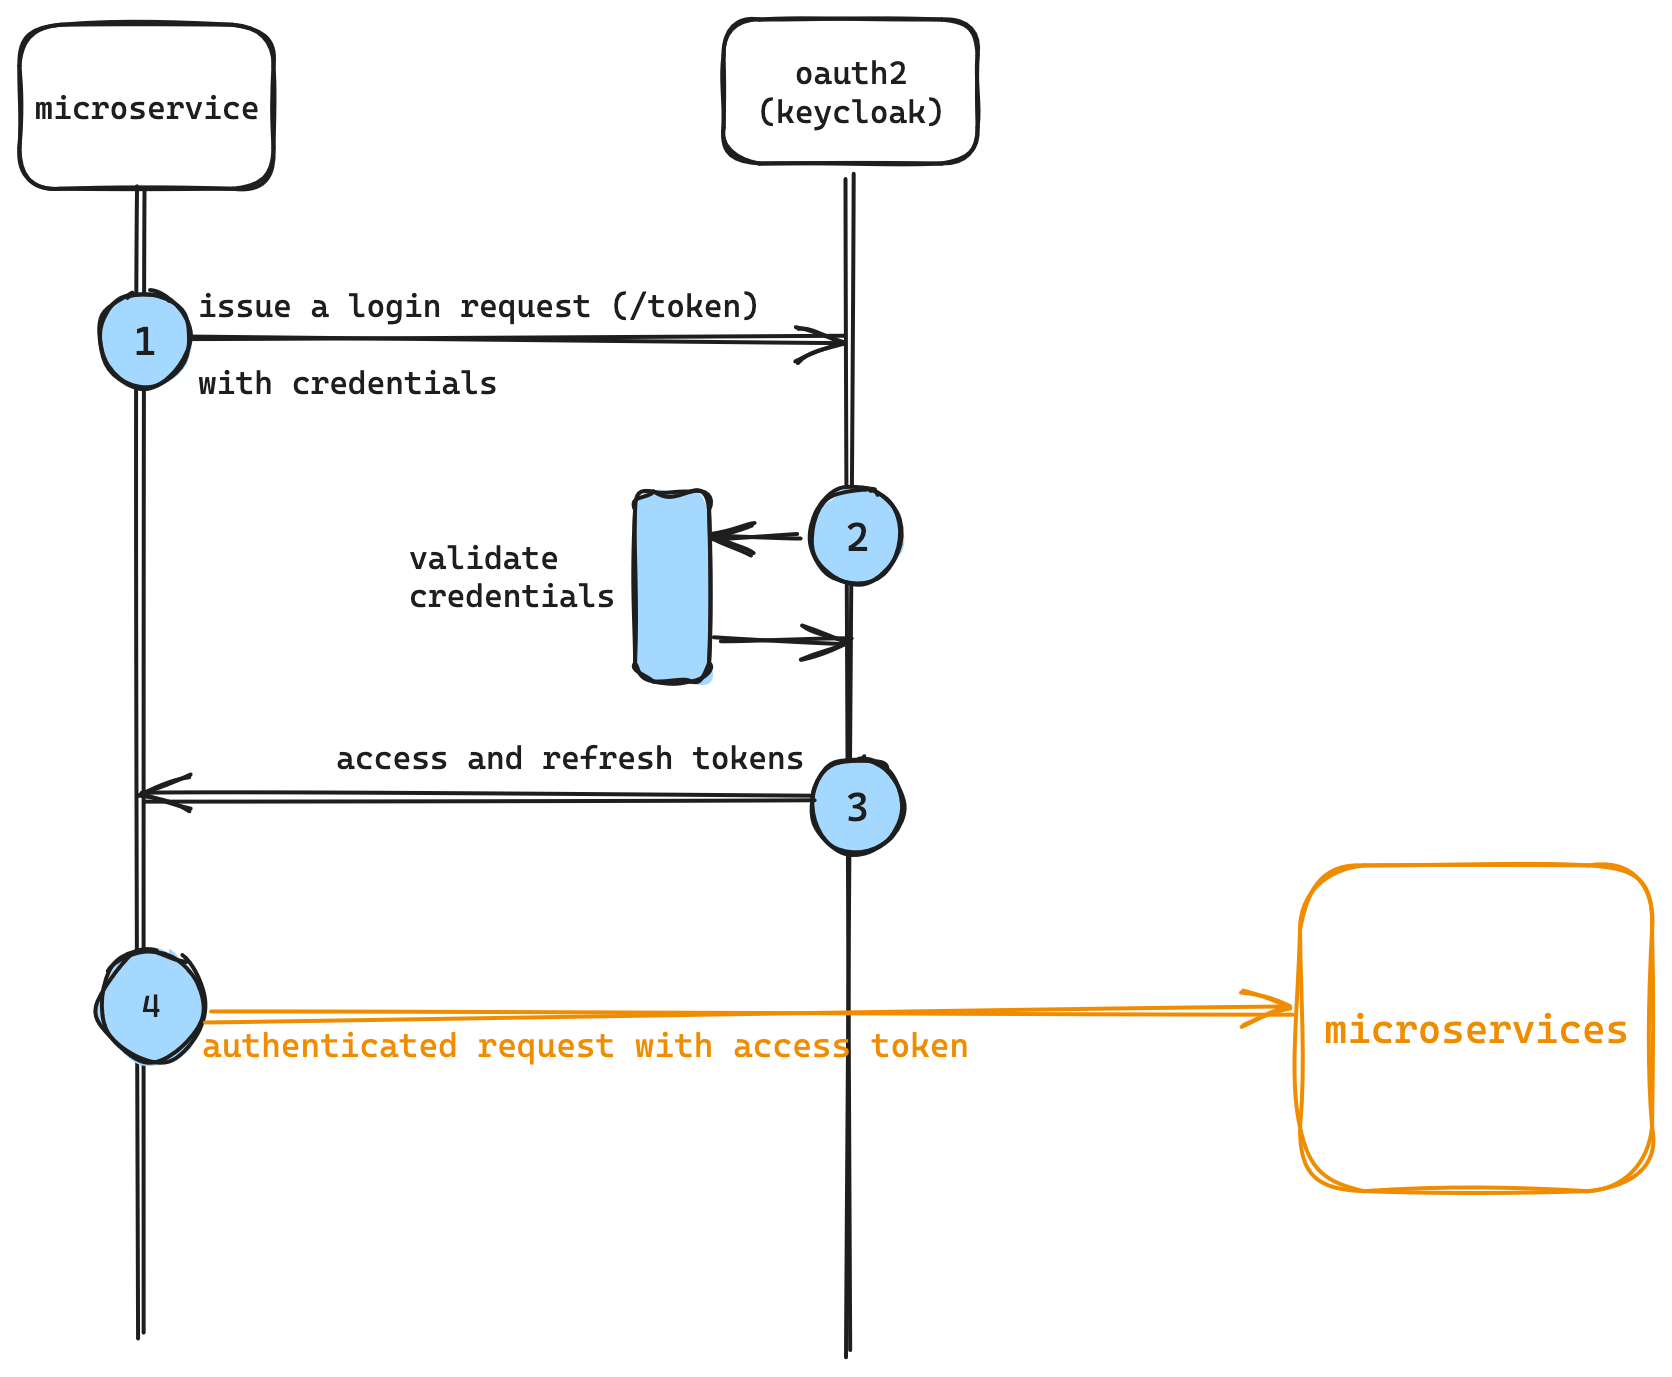
\includegraphics[width=1\textwidth]{files/images/service-account-flow.png}
    \caption{Service account flow}
    \label{fig:sa-flow}
\end{figure}
Come si può ben vedere, questo flusso è molto più semplice del precedente:
\begin{itemize}
    \item Il servizio ha delle credenziali pre-generate con le quali effettuare la richiesta per dei token;
    \item L'IDP valida le credenziali...
    \item ...e ritorna i token al servizio;
    \item In questo modo, il servizio in questione potrà effettuare richieste autenticate senza dover specificare sempre le proprie credenziali (come, ad esempio, succede con la \textit{Basic Auth}), riducendo la probabilità che queste vengano intercettate da agenti malevoli.
\end{itemize}

Per più dettagli sul funzionamento di questo protocollo e sulle attività ad esso riguardanti, è consigliabile consultare questo progetto\footnote{https://github.com/emilianomaccaferri/oauth2-spring-boot/tree/main}, di opera dell'autore di questa tesi.

\subsubsection{Keycloak}
Keycloak è una soluzione open-source di Identity and Access Management (IAM) sviluppata da Red Hat, progettata per semplificare l'autenticazione e l'autorizzazione nelle applicazioni moderne. Supporta protocolli standard come OpenID Connect, OAuth 2.0 e SAML 2.0, rendendolo compatibile con una vasta gamma di applicazioni e servizi. Keycloak consente di gestire centralmente utenti, ruoli, permessi e sessioni, offrendo funzionalità di Single Sign-On (SSO), federazione di identità, autenticazione a più fattori (MFA) e controllo di accesso basato su ruoli (RBAC). La sua architettura flessibile permette l'integrazione con directory LDAP, Active Directory, database relazionali e provider di identità esterni. Inoltre, Keycloak fornisce un'interfaccia utente web intuitiva per la gestione delle identità e offre API REST per l'integrazione programmatica.
\newline
Per via della sua estrema flessibilità e personalizzabilità, è stato scelto come \textit{IDP} per il progetto NextPyter.
\begin{figure}[h]
    \centering
    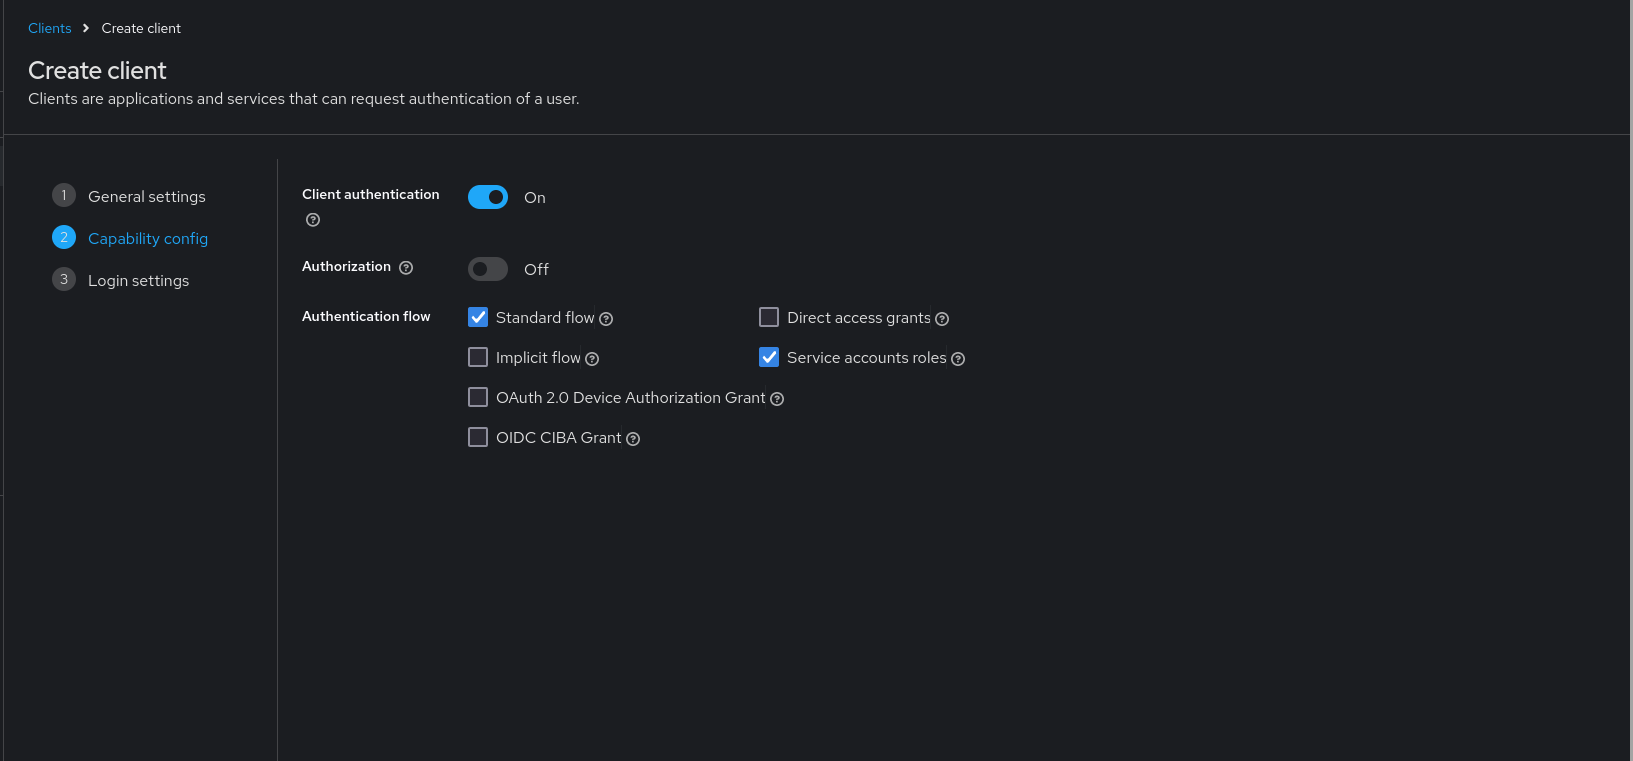
\includegraphics[width=1\textwidth]{files/images/keycloak.png}
    \caption{Una lista di flow supportati da Keycloak}
    \label{fig:keycloak-clients}
\end{figure}
\newline
In particolare, è possibile configurare Nextcloud in maniera tale che utilizzi un'istanza di Keycloak come provider di autenticazione e, di conseguenza, controllare le richieste e i permessi degli utenti dall'\textit{application gateway} citato in precedenza, poiché le credenziali che verranno emesse agli utenti di Keycloak saranno sotto forma di JWT, un formato di dati ispezionabile e crittograficamente verificabile.
\chapter{Realizzazione di NextPyter \textit{"2.0"}}
In questo capitolo verrà effettuata l'analisi tecnica dei componenti software del progetto NextPyter \textit{"2.0"}.
\newline
Saranno discussi, con codice e altri riferimenti, tutti i componenti \textit{core} e di autenticazione citati nella fase di progettazione, dando ampio spazio ad approfondimenti e commenti. 
\section{Rust come linguaggio di programmazione}
È stato scelto \textit{Rust}\footnote{https://rustlang.org} come linguaggio di programmazione per tutti i componenti di basso livello all'interno del \textit{core} di NextPyter per motivazioni riguardanti, principalmente, \textbf{prestazioni}, \textbf{\textit{type system} flessibile} e \textbf{facilità di distribuzione}. 
\newline
Rust è uno dei linguaggi più in diffusione del momento \cite{stackoverflow-2024}, possiede un ecosistema ricco di parecchie librerie che sfruttano le più recenti tecnologie in ambito di \textit{networking} e programmazione di sistema, offrendo moderni e affidabili strumenti per la soluzione di problemi in questi ambiti.
\newline
Grazie ad un moderno \textit{type system}, Rust è un linguaggio che permette di esprimere le relazioni fra i componenti di un programma in maniera estremamente chiara e, soprattutto, \textbf{type safe}. Questo significa che un programma compilato in Rust, che non fa uso di \textit{unsafe code}\footnote{https://doc.rust-lang.org/book/ch19-01-unsafe-rust.html}, ha la garanzia di non avere problemi riguardanti la null-safety e altri errori runtime riguardanti la gestione della memoria. Sempre grazie a queste \textit{feature}, Rust è in grado di garantire una velocità di esecuzione estremamente elevata, specialmente in ambienti riguardanti operazioni basate sull'I/O intensivo (come le applicazioni web) \cite{rust-perf}.
\newline
Siccome NextPyter riceverà potenzialmente parecchio traffico, è importante garantire che il suo ciclo di sviluppo sia quanto più lineare e riproducibile possibile e che gli applicativi che ne conseguiranno siano quanto più veloci possibili, garantendo i vincoli di resilienza e scalabilità di cui si parlava durante la fase di progettazione.
\newline
In conclusione, per via della mole di traffico che la piattaforma trattata è volta ad affrontare e dato il ruolo che i componenti \textit{core} andranno a ricoprire, le qualità di un linguaggio come Rust non andranno sprecate, anzi, brilleranno per la loro utilità in un sistema come NextPyter.
\section{Modulo \textit{daemon}}
In questa sezione verrà descritta la composizione del modulo \textit{daemon} di NextPyter, il componente di "rappresentanza", come già detto, di tutto il \textit{core}, ovvero quello che permetterà di interagire con le funzionalità della piattaforma.
\newline
La filosofia fondamentale alla base di questo componente è la sua \textit{statelessness}, ovvero la completa assenza di stato al suo interno, la cui gestione è delegata a componenti competenti. È molto importante capire che un componente così di facciata in un sistema del genere, deve essere in grado di gestire una quantità di traffico altamente variabile, quindi deve poter scalare in maniera completamente indipendente e \textbf{rapida} per garantire una corretta erogazione dei servizi di NextPyter.
\newline
Il codice è stato studiato appositamente per essere quanto più performante possibile, introducendo \textit{offloading}, quindi \textbf{delegazione}, di "compiti pesanti" in termini computazionali (come vederemo essere il download di immagini Docker, ad esempio) a componenti dell'architettura appositamente progettati.
\newline
In un certo senso, NextPyter è una piattaforma che segue la filosofia \textit{Unix}\footnote{https://en.wikipedia.org/wiki/Unix_philosophy}, predilgendo quindi il minimalismo e la modularità di un sistema, creando "piccoli" programmi che risolvono problemi specifici.
\newline
Il codice del modulo è consultabile a questo indirizzo: https://gitlab.com/nextpyter/daemon.
\subsection{Axum per la creazione di API REST}
Axum è un framework per la creazione di applicazioni web scritto in Rust, il cui focus sta sulla \textit{modularità} e riutilizzo del codice.
\newline
Questo framework, come tantissimi altri nel panorama \textit{Rust}, è basato su \textit{Tokio}\footnote{https://tokio.rs/}, un \textit{runtime} che permette la creazione di \textit{network application} asincrone, sfruttando le ultime tecnologie presenti nei kernel dei moderni sistemi operativi, rafforzando ancora di più le garanzie prestazionali che NextPyter si pone.
\newline
La base di tutte le applicazioni Axum è un \textit{router}, un componente dedicato alla gestione del traffico HTTP in arrivo all'applicazione Rust che farà utilizzo della libreria.
\newline
Ad un \textit{router} saranno associate più \textit{route}, sostanzialmente degli \textit{endpoint HTTP}, che assoceranno ad un determinato \textit{path}, ovvero un indirizzo, un URL, un determinato \textit{handler}, ovvero una funzione che si occuperà di gestire le richieste riguardanti quell'endpoint in particolare.
\newline
A scopo esemplificativo, ecco come è possibile creare una route con Axum:
\begin{verbatim}
use axum::{
    routing::{get, post},
    http::StatusCode,
    Json, Router,
};
use serde::{Deserialize, Serialize};

#[tokio::main]
async fn main() {

    // viene creato il router
    let app = Router::new()
        // viene registrata la coppia route - handler associata al path "/"
        .route("/", get(root));

    // viene associata una porta di ascolto 
    let listener = tokio::net::TcpListener::bind("0.0.0.0:3000").await.unwrap();
    axum::serve(listener, app).await.unwrap();
}

// l'handler della route specificata in precedenza è questo, che ritorna banalmente 
// un "Hello, World!" a scopo esemplificativo
async fn root() -> &'static str {
    "Hello, World!"
}
\end{verbatim}
\newpage
\subsection{Utilizzo di State per \textit{dependency injection}}
Per quanto riguarda la gestione delle dipendenze, Axum propone una soluzione particolarmente semplice da implementare, mediante il tipo \verb|State|. In questo modo, sarà possibile offrire, a tutte le route che ne necessiteranno, un oggetto contenente proprietà che possono essere usate per realizzare gli scopi dell'applicazione. In questo oggetto, generalmente, vengono messe le interfacce che regolano l'accesso al database e ad altri componenti "esterni" alle route, ma che queste ultime devono necessariamente interrogare.
\newline
A tale scopo, lo \verb|State| del modulo \textit{daemon} ha questo aspetto:
\begin{verbatim}
use std::{env, error::Error, sync::Arc};
use bollard::Docker;
use rqlite_rs::{RqliteClient, RqliteClientBuilder};
use serde::Deserialize;

use crate::libs::orchestrator::{...};

#[derive(Clone)]
pub struct AppState {
    pub orchestrator: Arc<Box<dyn Orchestrator>>,
    pub rqlite: Arc<RqliteClient>,
    pub redis: Option<redis::Client>, 
    pub images_stream_name: Option<String>,
}

pub async fn get_orchestrator(name: &str) -> Box<dyn Orchestrator> {
    match name {
        "kubernetes" => Box::new(KubernetesOrchestrator::new().await),
        "docker" => Box::new(DockerOrchestrator::new()),
        _ => panic!("no orchestrator found with that name!")
    }
}
impl AppState {
    pub async fn new(orchestrator_name: &str) -> Self {

        let rqlite = RqliteClientBuilder::new()
            .known_host(env::var("CONFIG_STORE_HOST")
            .unwrap_or("config-store:4001".to_string()))
            .auth(
                env::var("RQLITE_USER").unwrap().as_str(), 
                env::var("RQLITE_PASSWORD").unwrap().as_str()
            )
            .build()
            .expect("cannot create rqlite client");

        let images_stream_name = {
            if let Ok(res) = env::var("IMAGES_STREAM_NAME") {
                Some(res)
            }else {
                None
            }
        };

        let mut redis = None;
        if orchestrator_name.eq("docker") {
            redis = Some(
                redis::Client::open(env::var("REDIS_URI").unwrap())
                    .expect("cannot connect to redis")
            );
            assert!(images_stream_name.is_some());
        }

        AppState { 
            orchestrator: Arc::new(get_orchestrator(orchestrator_name).await),
            rqlite: Arc::new(rqlite),
            redis,
            images_stream_name
        }
    }
}
\end{verbatim}
In questa struttura dati, nel caso di NextPyter, è stato deciso di inserire le interfacce con l'orchestratore di container, che potrà essere Kubernetes o Docker (configurabile, come si può vedere, tramite variabili d'ambiente), l'interfaccia con il database distribuito, RQLite e l'interfaccia con \textit{Redis}/\textit{Valkey}, in modo tale che, al bisogno, le route potranno utilizzare questi oggetti per realizzare le logiche interne dettate dall'handler ad esse associate.
Utilizzare questa struttura dati è molto semplice, basta registrarla nel \textit{Router} (mediante l'apposito metodo \verb|with_state|, al quale viene passato l'oggetto contentente lo stato) e specificarla come argomento nelle \textit{route} che ne hanno necessità nel seguente modo:
\begin{verbatim}
pub async fn get_all_notebooks(
   State(s): State<AppState>,
) -> ... {
    s.orchestrator...
}
\end{verbatim}
Notare come lo \verb|State| venga "iniettato" nella route passandolo semplicemente come parametro. Questo paradigma non è da confondere con la dependency injection mediante IoC\footnote{https://www.baeldung.com/inversion-control-and-dependency-injection-in-spring}, come, ad esempio, quella presente in framework simili a Spring: la tecnica utilizzata si basa interamente sulla risoluzione dei tipi passati alle funzioni e tutte le dipendenze vengono risolte a tempo di compilazione, piuttosto che a runtime, garantendo performance straordinarie.
\newline
Sebbene non si entrerà nel dettaglio di questo paradigma, è importante sottolineare come questo approccio non solo permetta di \textbf{azzerare} un eventuale \textit{overhead} a runtime, ma riduce notevolmente le dimensioni del binario che si andrà eventualmente ad eseguire dopo la compilazione. Molti progetti basati su Rust fanno leva su questo paradigma: rendere la compilazione più "impegnativa" da un punto di vista computazionale, garantendo, però, performance runtime particolarmente elevate.
\newline
A scopo esemplificativo, è possibile vedere come è realizzato questo meccanismo in Axum direttamente dal codice sorgente della libreria\footnote{https://docs.rs/axum/latest/axum/handler/trait.Handler.html#implementors}: il \textit{trait}, un concetto assimilabile a quello di interfaccia per linguaggi OOP, \textit{Handler}, ovvero ciò che permette di definire come una richiesta viene interpretata a runtime, viene definito per \textit{molti tipi di chiamate a funzione}, ovvero \textit{molti tipi di handler}. A tempo di compilazione, per farla breve, il compilatore scansionerà tutti gli handler definiti da chi programma e verificherà che la loro definizione rispecchi una di quelle definite nella libreria; ovviamente questo è un processo abbastanza dispendioso, ma viene fatto a \textit{compile-time}, piuttosto che a \textit{runtime}, quindi viene eseguito una sola volta!
\newline
\subsection{Il trait \textit{Orchestrator}} \label{axum-orchestrator}
Come si può vedere, l'oggetto \verb|Orchestrator| è un \textit{trait}, assimilabile all'equivalente di un'interfaccia nei linguaggi OOP, che espone i seguenti metodi:
\begin{verbatim}
#[derive(Error, Debug)]
pub enum OrchestratorError {
    #[error("docker error: {0}")]
    DockerError(bollard::errors::Error),
    #[error("fatal error: {0}")]
    Generic(String),
    #[error("couldn't serialize: {0}")]
    SerializationError(String),
    #[error("kubernetes error: {0}")]
    KubernetesError(String),
}
// ... altro codice di contorno
pub trait Orchestrator: Send + Sync {
    async fn create_notebook_volume(
        &self, 
        container_name: &str, 
        path: &str
    ) -> Result<String, OrchestratorError>;

    async fn remove_notebook_volume(
        &self, 
        volume_name: &str, 
    ) -> Result<(), OrchestratorError>;

    async fn start_notebook_container(
        &self, 
        container_name: &str,
        container_image: &str,
        container_command: Vec<&str>,
        volume_name: &str,
        filename: Option<&str>,
    ) -> Result<String, OrchestratorError>;

    async fn get_all_notebook_containers_paginated(
        &self, 
    ) -> Result<Vec<NotebookDescription>, OrchestratorError>;

    async fn get_notebook_container(
        &self,
        container_name: &str,
    ) -> Result<Option<NotebookDescription>, OrchestratorError>;

    async fn stop_notebook_container(
        &self,
        container_name: &str
    ) -> Result<(), OrchestratorError>;

    async fn restart_notebook_container(
        &self,
        container_name: &str,
    ) -> Result<(), OrchestratorError>;

    async fn delete_notebook_container(
        &self,
        container_name: &str,
    ) -> Result<(), OrchestratorError>;

    async fn delete_notebook_container_data(
        &self,
        container_volume_name: &str,
    ) -> Result<(), OrchestratorError>;

}
\end{verbatim}
Come si può intuire, questo \textit{trait} verrà poi implementato in base al tipo di orchestratore che si andrà ad utilizzare, infatti esistono due implementazioni, una per Kubernetes e una per Docker:
\begin{verbatim}
// implementazione per Kubernetes
impl Orchestrator for KubernetesOrchestrator {
    ... 
    async fn get_notebook_container(
        &self, 
        container_name: &str,
    ) -> Result<Option<NotebookDescription>, OrchestratorError>{
        let pod_api: Api<Pod> = Api::namespaced(
            self.runtime.clone(), 
            &get_k8s_namespace()
        );
        let pod = pod_api.get_opt(&container_name).await?;
        dbg!(&pod);
        if let None = pod {
            return Ok(None)
        }

        Ok(Some(pod.unwrap().try_into()?))
    }

    ...
}

// implementazione per Docker
impl Orchestrator for DockerOrchestrator {
    async fn get_notebook_container(
        &self, 
        container_name: &str,
    ) -> Result<Option<NotebookDescription>, OrchestratorError>{
        
        let result = self.runtime.list_containers(Some(ListContainersOptions {
            filters: HashMap::from([
                ("name", vec![container_name]),
                ("status", vec!["running", "paused", "exited", "dead"])
            ]),
            ..Default::default()
        })).await?;
        
        if result.len() == 0 {
            return Ok(None)
        }
        if result.len() > 1 {
            warn!("{container_name} has been found multiple times?");
        }
    
        let found_container: NotebookDescription = result.first()
            .unwrap()
            .try_into()?;
    
        Ok(Some(found_container))
    }
    ...
}
\end{verbatim}
Anche senza una particolare esperienza con Rust, è facile capire che Orchestrator sarà un'interfaccia che esporrà metodi comuni che verranno utilizzati per astrarre il tipo di orchestratore con il quale \textit{daemon} andrà a comunicare.
\newline
Per astrarre le differenze che vi sono fra i due tipi di orchestratori e le loro interfacce, sono stati creati tipi appositi che vanno a "standardizzare" l'accesso alle risorse che servono per il corretto funzionamento del modulo. Sebbene entrambi gli orchestratori, Docker e Kubernetes, regolino le interazioni fatte da client esterni tramite l'utilizzo di una API REST, il formato dei dati è molto diverso, da cui ne deriva l'introduzione dei tipi di cui sopra.\newline
Il tipo \verb|NotebookDescription|, ad esempio, rappresenta l'implementazione di questo approccio:
\begin{verbatim}
#[derive(Serialize, Deserialize, ToSchema)]
pub struct NotebookDescription {
    pub notebook_id: String,
    pub notebook_endpoint: String,
    pub notebook_status: String,
    pub notebook_name: String,
}
\end{verbatim}
Il tipo "base" contiene informazioni che tutti i fruitori di questo tipo dovranno andare a poter leggere.
\newline
Grazie al moderno \textit{type system} di Rust è possibile andare a creare le implementazioni specifiche in maniera molto semplice:
\begin{verbatim}

// Docker

impl TryFrom<ContainerSummary> for NotebookDescription {

    type Error = NotebookDescriptionConversionError;
    
    fn try_from(container: ContainerSummary) -> Result<Self, Self::Error> {

        if let Some(id) = container.id.as_ref() {
            if let Some(names) = container.names.as_ref() {
                if let Some(notebook_name) = names.first() {
                    let notebook_name = &notebook_name[1..].to_string();
                    return Ok(NotebookDescription { 
                        notebook_id: id.to_string(),
                        notebook_name: notebook_name.clone(),
                        notebook_endpoint: build_notebook_uri(...),
                        notebook_status: container.status.clone()...,
                    })
                }
                return Err(NotebookDescriptionConversionError::EmptyNameError)            
            }
            return Err(NotebookDescriptionConversionError::NoNamesError)
        }
        Err(NotebookDescriptionConversionError::NoIdError)

    }
    
} 

// Kubernetes

impl TryInto<NotebookDescription> for Pod {
    type Error = NotebookDescriptionConversionError;

    fn try_into(self) -> Result<NotebookDescription, Self::Error> {

        if let Some(id) = &self.meta().name {
            if let Some(status) = &self.status {
                return Ok(NotebookDescription {
                    notebook_id: id.to_string(),
                    notebook_name: id.to_string(),
                    notebook_endpoint: build_notebook_uri(&id, None),
                    notebook_status: status.phase.clone()
                })
            }
            return Err(NotebookDescriptionConversionError::NoPodStatusError)
        }
        Err(NotebookDescriptionConversionError::NoIdError)
        
    }
}
\end{verbatim}
I due \textit{trait} \verb|TryFrom| e \verb|TryInto| permettono di fare casting \textit{type-safe}, nel senso che vengono date solide garanzie sull'implementazione del tipo di casting, tra i tipi \verb|NotebookDescritpion|, \verb|Pod|, ovvero la risorsa che contiene le informazioni sui container per quanto riguarda Kubernetes e \verb|ContainerSummary|, ovvero la stessa cosa, però in ambito Docker.
\newline
A questo punto sarà possibile derivare i tipi in maniera molto semplice e \textit{type-safe}!
\begin{verbatim}
// esempio con Docker
 async fn get_notebook_container(
        &self, 
        container_name: &str,
    ) -> ... {
        
        let result = self.runtime
            .list_containers(...).await?;
        // result è di tipo ContainerSummary
        
        // altri controlli omessi per chiarezza
    
        let found_container: NotebookDescription = result
            .first()
            .unwrap()
            .try_into()?;
        // esplicitando il tipo di dato nella definizione della
        // variabile, try_into() farà il casting
        // type safe specificato prima.
        // oltretutto, questo, a compile-time, ci darà
        // garanzie sul fatto che NotebookDescription
        // implementi correttamente il trait,
        // altrimenti il programma non compilerebbe!
        
        Ok(Some(found_container))
    }

\end{verbatim}
\subsection{Utilizzo di Bollard per l'interfaccia con Docker}
NextPyter, per interfacciarsi con Docker, utilizza una libreria Rust chiamata \textit{Bollard}\footnote{https://github.com/fussybeaver/bollard}, a sua volta basata su \textit{Tokio}, rendendo anche questa libreria completamente \textit{asincrona} e \textit{non bloccante}.
\newline
A seguire, nella sezione apposita, verrà commentata anche la libreria che \textit{daemon} usa per interfacciarsi con Kubernetes. 
\subsection{Struttura dell'API HTTP}
Per quanto riguarda la struttura dell'API HTTP, \textit{daemon} è composto da \textbf{due} principali route "madre": \verb|containers| e \verb|cfg|.
\begin{itemize}
    \item \verb|containers| conterrà tutte le route che riguardano il ciclo di vita dei container dei notebook che verranno generati all'interno della piattaforma NextPyter, sia su Docker che su Kubernetes, anche se quest'ultima parte avrà una sezione dedicata, per via della sua estensione;
    \item \verb|cfg|, invece, conterrà tutte le route che riguardano la configurazione dinamica delle immagini utilizzabili nel sistema e si interfaccerà con \textit{pagletto} per quanto riguarda l'offloading del download di queste ultime, per garantire la \textit{statelesness} del modulo \textit{daemon}. Questa serie di metodi, però, verrà descritta nella prossima sezione, per via della stretta relazione che ha con \textit{pagletto}.
\end{itemize}
\subsection{Analisi metodi containers}
I metodi disponibili per gestire i container nel sistema sono i seguenti:
\begin{verbatim}
Router::new()
    .route("/containers", get(root::index))
    .route(
        "/containers/stop/notebook/:container_name", 
        post(root::stop_notebook)
    )
    .route(
        "/containers/restart/notebook/:container_name", 
        post(root::restart_notebook)
    )
    .route("/containers/notebook/:container_name", get(root::get_notebook))
    .route(
        "/containers/notebook/:container_name", 
        delete(root::delete_notebook)
    )
    .route("/containers/notebook", post(root::spawn_notebook))
    .route("/containers/notebooks", get(root::get_all_notebooks));
\end{verbatim}
\subsubsection{Ottenere la lista di notebook nel sistema}
Mediante il metodo \verb|GET /containers/notebooks| è possibile ottenere una lista completa di tutti i notebook presenti nel sistema, attivi o meno.
\begin{verbatim}
pub async fn get_all_notebooks(
   State(s): State<AppState>,
) -> Result<Json<GetAllNotebooksResponse>, HttpError> {

    let all_notebooks = s.orchestrator
        .get_all_notebook_containers()
        .await?;

    Ok(Json(GetAllNotebooksResponse {
        success: true,
        count: all_notebooks.len(),
        containers: all_notebooks,
    }))

}
\end{verbatim}
In questo caso, \textit{daemon} interrogherà l'orchestratore, astratto dal tipo \verb|Orchestrator|, ricevendo tutte le informazioni necessarie per soddisfare la richiesta del client.
\subsubsection{Creazione di un notebook}
Mediante il metodo \verb|POST /containers/notebook| sarà possibile eseguire tutti gli step necessari per avviare correttamente un notebook sull'orchestratore configurato.
\begin{verbatim}
    pub async fn spawn_notebook(
    State(s): State<AppState>,
    // Token(user): Token<Claim<UserClaims>>,
    ValidatedJson(body): ValidatedJson<SpawnNotebookRequest>,
) -> Result<Json<SpawnNotebookResponse>, HttpError> {

    let SpawnNotebookRequest {
        folder_path,
        filename,
        image_id,
    } = body;

    let container_name = build_notebook_name(&nanoid!(24, &NANOID_ALPHABET));
    let notebook_token = nanoid!(32, &NANOID_ALPHABET);

    let volume_name = s.orchestrator
        .create_notebook_volume(&container_name, &folder_path).await?;

    let container_image = ContainerImage::from_id(
            & *s.rqlite, 
            &image_id
        ).await?;
    if container_image.is_none() {
        return Err(
            HttpError::Simple(
                StatusCode::NOT_FOUND, 
                "container_image_not_found".to_string()
            )
        )
    }
    let container_image = container_image.unwrap();
    
    let image_name = format!(
        "{}:{}", 
        &container_image.name, 
        &container_image.tag
    );
    
    let container_endpoint = s.orchestrator
        .start_notebook_container(
            &container_name,
            &image_name,
            vec!("start-notebook.sh",
                    ... // omesso per chiarezza
                ),
            &volume_name,
            filename.as_deref(),
        ).await?;

    Ok(
        Json(
            SpawnNotebookResponse {
                success: true,
                container_name,
                container_endpoint,
                notebook_token,
            }
        )
    )
}

\end{verbatim}
Anche qui si può notare che la struttura dei metodi di accesso agli orchestratori e, in questo punto fondamentale, l'accesso agli \textit{engine di storage} di questi ultimi, sia completamente uniforme e \textit{platform-agnostic}. Fra qualche sezione verrà descritto in maggiore dettaglio l'accesso allo \textit{storage} da parte di \textit{daemon}.

\subsubsection{Stop di un notebook}
Mediante il metodo \verb|POST /containers/stop/notebook/:container_name| sarà possibile eseguire tutti gli step necessari per fermare (ma non cancellare) l'esecuzione di un notebook.
\begin{verbatim}
pub async fn stop_notebook(
    State(s): State<AppState>,
    Path(StopNotebookParams { container_name }): Path<StopNotebookParams>
) -> Result<Json<GenericSuccessResponse>, HttpError> {

    if let Some(_) = s.orchestrator
        .get_notebook_container(&container_name)
        .await? {
            s.orchestrator.stop_notebook_container(&container_name).await?;
            Ok(
                Json(GenericSuccessResponse{
                    success: true,
                })
            )
    } else {
        return Err(
            HttpError::container_not_found_error()
        )
    }
    
}
\end{verbatim}
Notare come Rust sia estremamente moderno, con costrutti particolarmente intuitivi come \verb|if-let|, che pone particolare focus sulla \textit{null-safety} di questo linguaggio. 
\newline
In particolare, in Rust non esiste il valore \verb|null| per le variabili, rimpiazzato dal tipo \verb|Option<T>|. Sostanzialmente, quindi, le funzioni che possono non ritornare un valore (che in linguaggi come Java ritornerebbero \verb|null|, quindi), utilizzeranno questo tipo per esprimere la possibile mancanza di dati in ritorno; chi richiama la procedura, quindi, sarà forzato a controllare che sia stato ritornato qualcosa dalla funzione prima di procedere. 
\newline
Per capire meglio questa funzionalità è opportuno fare un esempio.
\newline
Le \textit{HashMap} in Rust sono implementate mediante il tipo \verb|Option<T>|:
\begin{verbatim}
use std::collections::HashMap;

fn main() {
    let mut map: HashMap<&str, u8> = HashMap::new();
    map.insert("key-1", 1);
    map.insert("key-2", 2);
    map.insert("key-3", 3);

    let maybe_value = map.get("key");
    if let Some(value) = maybe_value {
        println!("value: {:?}", value);
    }else{
        println!("no value found!");
    }
}
\end{verbatim}
In questo caso si è necessariamente forzati a controllare che all'interno di \verb|maybe_value| vi sia effettivamente un valore e non vi sia \verb|None| (l'alternativa a \verb|null|), in modo da prevenire che vengano utilizzati valori nulli, evitando completamente tutti i problemi relativi alle \textit{null-pointer exception}.
\newline
\verb|Option<T>|, infatti, è implementato nel seguente modo:
\begin{verbatim}
pub enum Option<T> {
    Some(T),
    None
}
\end{verbatim}
In altre parole, una funzione che fa utilizzo di \verb|Option<T>| potrà ritornare il valore effettivo all'interno del tipo \textit{wrapper} \verb|Some|, altrimenti \verb|None|, forzando a tempo di compilazione il controllo sul valore effettivo.\newline
Se Rust non avesse questo genere di costrutto, sarebbe possibile fare:
\begin{verbatim}
use std::collections::HashMap;

fn main() {
    let mut map: HashMap<&str, u8> = HashMap::new();
    map.insert("key-1", 1);
    map.insert("key-2", 2);
    map.insert("key-3", 3);

    let maybe_value = map.get("key");
    println!("value: {:?}", maybe_value);
}
\end{verbatim}
causando un errore runtime!
\subsubsection{Riavviare un container}
Mediante il metodo \verb|POST /containers/restart/notebook/:container_name| sarà possibile riavviare un notebook in esecuzione.
\begin{verbatim}
pub async fn restart_notebook(
    State(s): State<AppState>,
    Path(RestartNotebookParams{ container_name }): Path<RestartNotebookParams>
) -> Result<Json<GenericSuccessResponse>, HttpError> {

    if let Some(_) = s.orchestrator.get_notebook_container(&container_name).await? {
        s.orchestrator.restart_notebook_container(&container_name).await?;

        Ok(
            Json(GenericSuccessResponse{
                success: true,
            })
        )
    } else {
        return Err(
            HttpError::container_not_found_error()
        )
    }

}

\end{verbatim}
\subsubsection{Rimozione permanente di un notebook}
Mediante il metodo \verb|DELETE /containers/notebook/:container_name| sarà possibile rimuovere permanentemente un notebook dal sistema.
\begin{verbatim}
pub async fn delete_notebook(
    State(s): State<AppState>,
    Path(DeleteNotebookParams{ container_name }): Path<DeleteNotebookParams>
) -> Result<Json<GenericSuccessResponse>, HttpError>{

    if let Some(notebook) = s.orchestrator
        .get_notebook_container(&container_name)
        .await? {

            s.orchestrator
                .stop_notebook_container(&notebook.notebook_name).await?;
            s.orchestrator
                .delete_notebook_container(&notebook.notebook_name).await?;
            s.orchestrator
                .delete_notebook_container_data(
                &build_volume_name(&notebook.notebook_name)
            ).await?;
    
        Ok(
            Json(GenericSuccessResponse {
                success: true,
            })
        )
    } else {
        return Err(
            HttpError::container_not_found_error()
        )
    }
}

\end{verbatim}
\newpage
\subsection{Documentazione autogenerante con \textit{utoipa}}
Per rendere il processo di documentazione quanto più integrato nel ciclo di sviluppo, si è utilizzato \verb|utoipa|, una libreria che auto-genera documentazione a partire da determinate \textit{macro}, ovvero particolari direttive al compilatore Rust, di \textit{code-generation}.
\newline
Decorare una \textit{route} con la documentazione è molto semplice, come si può vedere dal seguente esempio:
\begin{verbatim}
#[utoipa::path(
    post,
    path = "/containers/notebook",
    responses(
        (
            status = 200, 
            description = "Container spawned successfully", 
            body = SpawnNotebookResponse,
        ),
        (
            status = 404,
            description = "Container not found",
        )
    ),
    security(
        ("bearerAuth" = [])
    ),
    request_body(
        content_type = "application/json", content = SpawnNotebookRequest
    )
)]
pub async fn spawn_notebook(
    State(s): State<AppState>,
    ValidatedJson(body): ValidatedJson<SpawnNotebookRequest>,
) -> Result<Json<SpawnNotebookResponse>, HttpError> {
    ...
}
\end{verbatim}
Mediante la macro \verb|#[utoipa::path()]| è possibile istruire il compilatore alla generazione di uno schema \textit{OpenApi v3}. In questo caso verrà generato uno schema di una richiesta \verb|POST|, con URI \verb|/containers/notebook| e poi verrà elencata una lista di risposte possibili. Notare come è possibile passare un tipo personalizzato tra queste ultime, in questo caso \verb|SpawnNotebookResponse|:
\begin{verbatim}
use serde::Serialize;
use utoipa::{ToResponse, ToSchema};

#[derive(Serialize, ToResponse, ToSchema)]
#[response(description="...")]
pub struct SpawnNotebookResponse {
    #[schema(example = true)]
    pub success: bool,
    #[schema(example = "notebook-hfxKMA4gvZ-74l7ZC3b3Wnym")]
    pub container_name: String,
    #[schema(example = "http://proxy-uri:8080/notebook/...")]
    pub container_endpoint: String,
    #[schema(example = "KwODErMig4oZFPAPuYbXG1ug26lSgp4-")]
    pub notebook_token: String,
}
\end{verbatim}
Derivando, tramite, anche qui, particolari \textit{macro} di \verb|utoipa|, i \textit{trait} \verb|ToResponse| e \verb|ToSchema|, è possibile andare ad arricchire il nostro tipo con metadati che verranno estrapolati a tempo di compilazione, ovvero quando queste \textit{macro} verranno eseguite. In particolare, tramite la macro \verb|#[schema()]| è possibile andare ad inserire commenti sui tipi di dato che compariranno nella documentazione. 
\newline
A questo punto sarà possibile esporre la documentazione autogenerata in maniera molto semplice, facendo uso di una \textit{route} apposita:
\begin{verbatim}
async fn build_json_schema() -> impl IntoResponse {

    let str_docs = ApiDoc::openapi()
        .to_pretty_json()
        .unwrap();
    let mut headers = HeaderMap::new();
    headers.insert("Content-Type", "application/json".parse().unwrap());

    (headers, str_docs)

}

// omesso per brevità

let app = Router::new()
        .route("/", get(routes::main::root::index))
        .route("/json-schema", get(build_json_schema))
        .with_state(state.clone())
        .merge(container_routes(state.clone()))
        .merge(cfg_routes(state.clone()));
\end{verbatim}
Dall'esempio di codice si può capire che la documentazione sarà esposta sull'endpoint \verb|/json-schema|.
\newpage
\section{Modulo \textit{pagletto}}
Per supportare la possibilità di scaricare immagini Docker "on-demand", direttamente dalla piattaforma, è stato necessario introdurre un secondo modulo, \textit{pagletto}, per due principali motivi: il primo è sicuramente per mantenere quanto più modulare e \textit{non-monolitico} il progetto, riducendo la responsabilità che ciascun componente ha, mentre il secondo riguarda la natura stessa della funzionalità che si è voluto introdurre; scaricare immagini Docker è un processo potenzialmente molto lungo (alcune immagini possono avere dimensioni nell'ordine dei gigabyte), pertanto per non appesantire computazionalmente il modulo \textit{daemon} con task che, eventualmente, potrebbero andare a saturare la sua threadpool, è stato introdotto \textit{pagletto}.
\newline
Questo modulo è concettualmente molto semplice, tutto quello che fa è:
\begin{itemize}
    \item attendere che \textit{daemon} indichi la necessità di scaricare una nuova immagine Docker;
    \item una volta ricevuto questo segnale, si andrà a scaricare tale immagine;
    \item quando l'immagine è stata scaricata, si registrerà come "disponibile" una nuova immagine da utilizzare su NextPyter;
    \item qualora vi siano degli errori durante il download, eventualmente riprovare il task in futuro.
\end{itemize}
Le tecnologie a supporto del modulo sono \textit{Valkey}, un database \textit{key-value} che verrà utilizzato come \textit{broker} di eventi, e \textit{RQLite}, il database \textit{highly available} che verrà utilizzato per memorizzare la configurazione di NextPyter, quindi le immagini disponibili.
\subsection{Utilizzo di Valkey e Valkey Streams per collegare \textit{daemon} e \textit{pagletto}}
Per creare la dinamica di "attesa-e-risposta" citata precedentemente, è stato necessario introdurre un componente che facesse da "ponte" tra i due moduli, Valkey,  un \textit{key-value} store ad altissime performance che da qualche anno supporta anche la possibilità di creare dei cosiddetti \textit{stream}: uno \textit{stream} è una struttura dati, assimilabile concettualmente ad una lista \textit{append-only}, dalla quale, all'inserimento di un dato al suo interno, verranno emessi eventi verso eventuali consumatori di tale struttura dati.\newline
In particolare, Valkey supporta due principali modalità:
\begin{itemize}
    \item \textit{Fan-out}: uno stream può essere controllato da \textit{N} consumatori. All'inserimento di un \textit{record} all'interno dello stream, \textbf{tutti} i consumatori verranno notificati, processando il messaggio parallelamente;
    \item \textit{Consumer groups}: questa modalità viene utilizzata quando ciascun consumatore dovrà essere il \textbf{solo} a ricevere un determinato messaggio. In altre parole, Valkey agirà in modo tale che tutti gli elementi che vengono inseriti all'interno dello stream verranno processati, a turno, da un singolo consumatore. Supponendo, ad esempio, di avere tre consumatori \textit{(C1, C2, C3)} e supponendo di ricevere messaggi numerati da 1 a 7, la sequenza di ricezione messaggi sarà:
        \begin{verbatim}
1 -> C1
2 -> C2
3 -> C3
4 -> C1
5 -> C2
6 -> C3
7 -> C1
        \end{verbatim}
    In questo caso, Valkey supporta un meccanismo di \textit{acknowledgement} per distinguere i messaggi processati correttamente da quelli malformati e/o con errori. Questa strategia permette di implementare policy di \textit{retry} da parte dei consumer dello stream qualora qualcosa vada storto durante il processing del messaggio.
\end{itemize}

\subsection{Funzionamento consumer groups}
Per modellare i requisiti specificati, è stato creato uno stream chiamato \verb|stream:image_data|, configurato come consumer group, mediante il seguente comando:
\begin{verbatim}
    XGROUP CREATE stream:image_data builders $ MKSTREAM
\end{verbatim}
Tramite questo comando vengono creati al contempo lo stream, \verb|stream:image_data|, e il gruppo di consumatori che andrà ad accedere a tale stream, \verb|builders|; tutti i client che vorranno connettersi a tale stream dovranno specificare esplicitamente il gruppo di riferimento. Ovviamente è possibile associare più gruppi ad uno stream, creando parallelismo \textbf{tra} i gruppi, ma non competizione, poiché le logiche di \textit{acknowledgement} hanno luogo \textbf{all'interno} di un consumer group.
\newline
\subsubsection{Aggiunta dati ad uno stream}
Aggiungere dati ad uno stream è particolarmente facile:
\begin{verbatim}
    XADD 
        <nome stream> 
        <id entry dello stream> 
        <key1> <value1> 
        <key2> <value2> 
        <key3> ...
\end{verbatim}
Ad esempio, per aggiungere un oggetto all'interno dello stream creato in precedenza: 
\begin{verbatim}
    XADD 
        stream:image_data 
        * 
        image_name nginx 
        image_version mainline 
        job_id aab3ef3fb33b2cecafabc3d3b3bab
\end{verbatim}
In questo caso verrà aggiunta una nuova \textit{entry} nello stream con id autogenerato (tramite il carattere \verb|*|). La entry sarà assimilabile ad una mappa con i seguenti valori:
\begin{verbatim}
    {
        "image_name": "nginx",
        "image_version": "mainline",
        "job_id": "aab3ef3fb33b2cecafabc3d3b3bab"
    }
\end{verbatim}
\subsubsection{Lettura dati da uno stream configurato come \textit{consumer group}}
Anche leggere dati da uno stream configurato come \textit{consumer group} è immediato: 
\begin{verbatim}
    XREADGROUP 
        GROUP
        <group-name>  
        BLOCK
        <block-time>
        <consumer-names> 
        STREAMS 
        <stream-name> 
        <start-index>
\end{verbatim}
\begin{itemize}
    \item il parametro \textbf{start-index} indica l'indice del messaggio da cui iniziare la lettura dello stream. Questo parametro supporta dei particolari valori:
        \begin{itemize}
            \item \verb|>|: questo valore indica la volontà da parte del consumer di voler leggere \textit{solo i nuovi messaggi}, quindi praticamente significa "ascoltare in tempo reale" ciò che accade sullo stream;
            \item  \verb|"0-0"|: questo valore indica, invece, la volontà di leggere lo stream a partire dal \textit{primo elemento}. Questo è utile in fase di inizializzazione di \textit{pagletto}, poiché permette di processare tutti i messaggi di \textit{backlog}, ovvero quelli inseriti quando i consumer non erano disponibili (se un client mette un messaggio nello stream senza che nessun consumer sia attivo, questo rimarrà nella cosiddetta \textit{backlog} dello stream).
        \end{itemize}
    \item il parametro \textbf{block-time}, invece, indica quanti millisecondi il consumer deve aspettare prima di leggere lo stream: questo \textit{delay} viene applicato per non occupare inutilmente la coda di task asincroni di \textit{Tokio}.
    \item è facile intuire cosa rappresentino gli altri parametri.
\end{itemize}
\subsubsection{\textit{Acknowledgement} e \textit{autoclaiming}}
\textit{Acknowledgement} e \textit{autoclaiming} sono i due meccanismi che permettono ai consumer di implementare meccanismi di \textit{retry} qualora il processamento di un messaggio non vada a buon fine.
\newline
Il comando usato per fare \textit{acknowledgement} di un messaggio è molto semplice:
\begin{verbatim}
    XACK
        <stream-name>
        <group-name>
        <message-id>
\end{verbatim}
Fare \textit{acknowledgement} di un messaggio significa rimuoverlo dalla coda dei messaggi \textit{pending} (quindi dallo stream), ovvero quelli ancora in fase di processamento o ancora da processare. In questo modo, una volta che si fa \textit{ack} di un messaggio, questo verrà rimosso dalla lista di messaggi che vengono letti tramite il comando \verb|XREAD|.
\newline
Tramite il comando \verb|XAUTOCLAIM|, invece, è possibile \textbf{recuperare messaggi}. È possibile, infatti, che alcuni \textit{consumer} all'interno di un gruppo non riescano a processare un messaggio: quando questo è il caso, sarà necessario che quel messaggio venga recuperato in un qualche modo e venga ri-processato da un altro consumer.
\begin{verbatim}
    XAUTOCLAIM 
        <stream-name> 
        <group-name>
        <consumer>
        <min-idle-time> 
        <start>
\end{verbatim}
Il parametro \textbf{min-idle-time} indica sostanzialmente il numero di millisecondi che devono essere passati dall'ultimo \verb|CLAIM| di un messaggio. Il \verb|CLAIM| di un messaggio avviene quando viene \textit{letto} tramite \verb|XREAD|, ma può anche avvenire manualmente mediante l'utilizzo del comando \verb|XCLAIM|. Pertanto, se questo comando viene chiamato in questo modo:
    \begin{verbatim}
    XAUTOCLAIM
        streams:image_data
        builders
        builder-1
        60000
        "0-0"
    \end{verbatim}
ciò significherà che il consumer \verb|builder-1| partirà dall'inizio dello stream (\verb|"0-0"|) e controllerà che vi siano messaggi con età maggiore di un minuto. Il consumer in questione si impossesserà dei messaggi e farà un \verb|CLAIM| implicito di questi ultimi. A questo punto, i messaggi appena ottenuti saranno disponibili nella prossima chiamata ad \verb|XREAD|.
\newline
In altre parole, se un messaggio non viene \textit{acknowledged} e non viene effettuato il \textit{re-claim} dal consumer che l'ha inizialmente letto entro un intervallo minore di quello specificato in \verb|XAUTOCLAIM|, allora questo messaggio verrà "rimosso" dalla coda del consumer iniziale e verrà assegnato a quello che fa quest'ultimo comando, permettendo il \textit{ri-processamento} di messaggi che hanno avuto problemi.
\subsection{Comunicazione tra \textit{daemon} e \textit{pagletto}}
Assodato il concetto di \textit{stream}, è ora venuto il momento di dettagliare come i due moduli si connettono.
\subsubsection{Route \textit{cfg}}
Come anticipato, le route che dipendono dalla route "madre" \verb|cfg| sono quelle che regolano la configurazione del sistema.
\begin{verbatim}
    Router::new()
        .route("/cfg/request-image-pull", post(root::request_image_pull))
        .route("/cfg/image-logs/:image_id", get(root::get_image_logs))
        .route("/cfg/images", get(root::get_images))
        .with_state(state)
\end{verbatim}

\subsubsection{Richiedere il download di un'immagine}
Tramite la route \verb|POST /cfg/request-image-pull| è possibile iniziare il download di un'immagine Docker.
\begin{verbatim}
pub async fn request_image_pull(
    State(s): State<AppState>,
    ValidatedJson(body): ValidatedJson<PullImageRequest>
) -> Result<Json<PullImageResponse>, HttpError> {

    let PullImageRequest {
        image_name,
        image_tag
    } = body;

    let image_id = nanoid!(32);
    let mut conn = s
        .redis.unwrap()
        .get_multiplexed_async_connection()
        .await?;
        
    redis::cmd("xadd")
        .arg(s.images_stream_name.unwrap())
        .arg("*")
        .arg("image_name")
        .arg(&image_name)
        .arg("image_tag")
        .arg(&image_tag)
        .arg("job_id")
        .arg(&image_id)
        .query_async(&mut conn)
        .await?;


    Ok(Json(
        PullImageResponse {
            success: true,
            image_id
        }
    ))

}

\end{verbatim}
Come si può evincere da questo spezzone di codice, la route non farà altro che piazzare un messaggio all'interno di uno \textit{stream} Valkey, in maniera del tutto analoga a quella vista nella sezione precedente. A valle, vi sarà \textit{pagletto} che riceverà questo aggiornamento e processerà questo evento. Avremo modo di approfondire \textit{come} avviene il download da parte di \textit{pagletto} tra un paio di paragrafi.

\subsubsection{Stato di un'immagine}
Tramite la route \verb|GET /cfg/image-logs/:image_id| è possibile monitorare lo stato di avanzamento del processo di download dell'immagine.
\begin{verbatim}
pub async fn get_image_logs(
    State(s): State<AppState>,
    Path(GetImageLogsParams { image_id }): Path<GetImageLogsParams>
) -> Result<Json<GetImageLogsResponse>, HttpError> {

    let result = ContainerImage::get_logs(
        & *s.rqlite,
        &image_id
    ).await?;

    Ok(Json(
        GetImageLogsResponse {
            success: true,
            result,
        }
    ))

}

\end{verbatim}
Anche qui si fa uso di \textit{RQLite} per persistere questi log in maniera ridondata. Tramite questo endpoint si potrà verificare se vi sono stati errori durante il download o se tutto è andato liscio.

\subsection{Schema di funzionamento di \textit{pagletto}}
Nel seguente diagramma è riassunto lo schema di funzionamento di \textit{pagletto}. È stato scelto questo metodo per rappresentarne il funzionamento, perché questo modulo è particolarmente di basso livello e andrebbero introdotti concetti che vanno al di fuori dello scopo di questa tesi.
\begin{figure}[h]
    \centering
    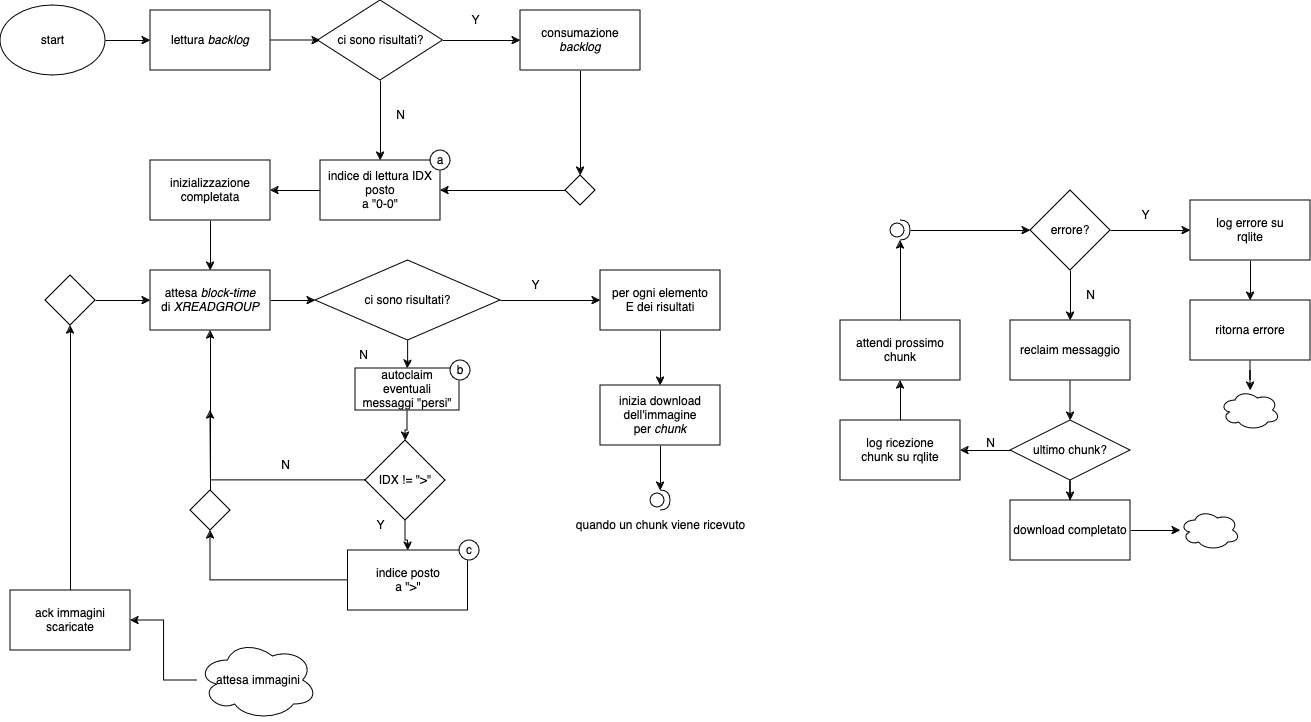
\includegraphics[width=1\textwidth]{files/images/pagletto-diagram.jpg}
    \caption{Schema di funzionamento di \textit{pagletto}}
    \label{fig:pagletto-diagram}
\end{figure}
\begin{itemize}
    \item nel punto \verb|a|, notiamo che l'indice di lettura viene posto a "0-0" e non a ">". Questo perché è possibile che durante l'operazione di lettura della \textit{backlog} siano arrivati dei messaggi che non possono essere saltati, ma che vanno processati.
    \item punto \verb|b|: questo viene effettuato perché viene data precedenza ai messaggi in arrivo in tempo reale. Quando non vi sono messaggi in arrivo, allora si processano quelli nella cosiddetta \textit{dead-letter queue};
    \item punto \verb|c|: qualora non vi sia alcun messaggio, né nella \textit{dead-letter queue} né dalla lettura dell'indice "0-0", allora ci si mette in ascolto di nuovi messaggi.
\end{itemize}

Nonostante il componente \textit{pagletto} sia stato realizzato per fare \textit{offloading} del download delle immagini, è stata comunque prestata attenzione alla metodologia di gestione di questo task: se si nota, infatti, il download avviene in maniera particolarmente efficiente in un contesto asincrono, dato che i chunk del download vengono processati indipendentemente e collezionati alla fine del download, permettendo di gestire tanti task alla volta.
\newline
Per più dettagli sul funzionamento di questo modulo, è opportuno consultare la repo di riferimento\footnote{https://gitlab.com/nextpyter/pagletto}.
\newpage
\section{Modulo \textit{proxy}}
Il modulo \textit{proxy} è particolarmente importante per quanto riguarda l'implementazione di logiche di \textit{routing} personalizzate del traffico che proviene dall'esterno verso il \textit{core} di NextPyter. 
\newline
La tecnologia abilitante alla base di questo modulo è \textit{NGINX}, come già anticipato, con supporto a \textit{NJS}.
\subsection{Configurazione di NGINX come reverse proxy per notebook Jupyter}
Il principale risultato che si vuole ottenere tramite questa configurazione è quello già mostrato in figura \ref{fig:routing}, che risolve principalmente la questione riguardante il \textit{binding} della porta locale: si vuole evitare di dover associare ciascun notebook ad una porta locale dell'host, in modo da far passare il traffico per quella porta. Questo setup, oltre che ad essere controproducente per i motivi elencati nella sezione \ref{net-acceptable}, non è facilmente realizzabile in un sistema basato su Kubernetes, poiché il \textit{network model}\footnote{https://kubernetes.io/docs/concepts/services-networking/} che quest'ultimo implementa si basa su astrazioni più complesse di quelle di Docker.
\newline
\subsubsection{Come configurare NGINX}
Prima di spiegare la configurazione effettiva di NGINX per NextPyter è opportuno introdurre alcuni concetti riguardanti quest'ultima.
\newline
A tale pro, ecco un semplicissimo \textit{setup}:
\begin{verbatim}
server {
    listen 14000;
    resolver 127.0.0.11 ipv6 off;
}
\end{verbatim}
I file di configurazione per NGINX funzionano a "blocchi", ovvero sezioni di testo racchiuse fra parentesi graffe:
\begin{itemize}
    \item il blocco \verb|server| specifica che si sta scrivendo una configurazione per un determinato dominio o host. Questo concetto è chiamato \textit{virtualhosting}, che sostanzialmente è riassumibile come la capacità di un web server di gestire tanti domini per volta. NGINX implementa questa funzionalità separando ogni configurazione di dominio all'interno di file differenti (o, volendo, all'interno di blocchi \verb|server| all'interno dello stesso file). Generalmente, una configurazione si riferisce ad un determinato dominio tramite la direttiva \verb|server_name|, quindi se ad esempio si vuole scrivere la configurazione per il dominio \verb|macca.cloud|, andrà specificato \verb|server_name macca.cloud|. Se si omette tale direttiva, come nella configurazione d'esempio, il blocco \verb|server| di riferimento agirà come \textit{"catch-all" route}, ovvero la \textit{route} alla quale tutte le richieste che fanno riferimento a domini non gestiti da NGINX verrano redirette.\newline
    Poiché non vi sono domini, dato che questo è un proxy interno al \textit{core} di NextPyter, è possibile omettere la direttiva \verb|server_name|, anche perché questo sarà l'unico file di configurazione che verrà scritto;
    \item Con la direttiva \verb|listen|, invece, si associa NGINX ad una porta locale. In questo caso, NGINX sarà dentro un container, pertanto bisognerà esporre tale porta, locale al container, in un qualche modo, che dipenderà dall'orchestratore che sta sotto il sistema;
    \item La direttiva \verb|resolver| è di fondamentale importanza in ambienti containerizzati, sia su Kubernetes che su Docker, poiché tramite questa sarà possibile utilizzare i \textbf{nomi dei container} al posto dei loro IP anche nelle configurazioni di NGINX. Questo è particolarmente utile poiché gli indirizzi di rete dei container, sia in Docker che in Kubernetes, sono \textit{ephemeral}, nel senso che non sono allocati con una particolare persistenza, pertanto non si può fare alcuna assunzione sul loro valore tra un riavvio di container e l'altro.
\end{itemize}
Una configurazione più avanzata può introdurre il concetto di \textit|location|, che si definirà con un blocco che avrà lo stesso nome. Le \textit{location} sono sostanzialmente il concetto di \textit{route} che è già stato descritto quando si è parlato di \textit{Axum}, ma "tradotte" nel linguaggio di configurazione NGINX.
\begin{verbatim}
server{
    listen 14000;
    # resolver, ...

    location /something/ {

        proxy_pass http://service-inside-docker:8080/;
    }

    # ... more stuff
}
\end{verbatim}
\begin{itemize}
    \item Usando il blocco \verb|location|, quindi, si avrà la possibilità di creare una nuova \textit{route} verso la quale si potranno fare richieste HTTP. In questo esempio è stata creata la route \verb|/something/|, che sostanzialmente si occuperà di gestire tutte le richieste di tipo \verb|http://localhost:14000/something/*|. Notare come il \textit{trailing slash} sia di fondamentale importanza, perché abilita proprio questo comportamento;
    \item All'interno del blocco \verb|location| viene descritto ciò che accade quando una richiesta che viene "catturata" dalla location:
        \begin{itemize}
            \item \verb|proxy_pass| imposta l'indirizzo verso il quale si vogliono re-indirizzare le richieste. In questo caso, il \textit{trailing slash}, oltre ad attivare il meccanismo succitato, farà in modo che NGINX passi verso l'indirizzo specificato \textit{tutto l'URI}. Ad esempio, se la richiesta fosse \newline\verb|http://localhost:14000/something/a/b/c|, allora NGINX indirizzerebbe tale richiesta a \verb|http://service-inside-docker:8080/a/b/c| (notare come viene \textbf{omesso} il path della \verb|location|!). 
        \end{itemize}
\end{itemize}
Sono state descritte le direttive che verranno utilizzate all'interno di NextPyter, ma, ovviamente, NGINX può fare molto più di quello che è scritto in questa breve introduzione.
\newline
Un'ultieriore osservazione può essere fatta sull'indirizzo che è specificato nella direttiva \verb|proxy_pass|: quell'indirizzo è un \textit{nome DNS}, non un indirizzo IP, pertanto è necessario configurare NGINX, come si è visto in precedenza, in modo tale che supporti un \textit{resolver} che contenga tale nome. Di uguale importanza è il fatto che tutti i servizi che vengono raggiunti in questo modo \textbf{dovranno essere già online} quando NGINX caricherà questa configurazione, perché dovranno essere risolti in modo da associarvi un IP.
\subsubsection{Reverse proxy per i notebook} \label{reverse-proxy-oauth}
La configurazione precedente si basa su un \textit{matching statico}, nel senso che sia la \verb|location| che la direttiva \verb|proxy_pass| agiscono su stringhe \textit{statiche}: tutte le richieste che soddisfano il path \verb|/something/*| verranno \textit{sempre} reindirizzate a \newline\verb|http://service-inside-docker:8080/*|.\newline
Poiché i nomi dei notebook, quando eseguiti da \textit{daemon}, sono generati randomicamente e in una maniera non deterministica, è necessario introdurre il concetto di \textit{pattern matching} all'interno dei blocchi \verb|location|.\newline
Ipotizzando che gli URL dei notebook avranno forma del tipo
\begin{verbatim}
    /notebook/nome-notebook/path-qualsiasi?parametro=a&altro-parametro=b
\end{verbatim}
e sapendo che il nome del notebook equivale al suo \textbf{nome DNS} all'interno dell'orchestratore, il problema può essere risolto in questo modo:

\begin{verbatim}
location ~ ^/notebook/([^/]+)/(.*)$ { 
                
    proxy_pass http://$1:15750;

    # altri header di configurazione, non verranno commentati perché
    # fuori dallo scopo di questa sezione, anche perché sono
    # abbastanza standard
    proxy_set_header Host $http_host;
    proxy_set_header X-Real-IP $remote_addr;
    proxy_set_header X-Forwarded-For $proxy_add_x_forwarded_for;
    proxy_set_header X-Forwarded-Proto $scheme;
    proxy_http_version 1.1;
    proxy_redirect off;
    proxy_buffering off;
    proxy_set_header Upgrade $http_upgrade;
    proxy_set_header Connection "upgrade";
    proxy_read_timeout 86400;

}
\end{verbatim}
In particolare, è importante notare che la \verb|location| è sostanzialmente definita tramite una \textit{regex}: tutti gli URL che hanno la forma succitata subiranno il seguente trattamento:
\begin{itemize}
    \item tramite il primo \textit{capture group}, ovvero \verb|([^/]+)|, verrà estratta la prima parte dell'URL, ovvero il \textbf{nome del container}. Questo risultato sarà inserito nella variabile \verb|$1| interna alla \verb|location| (comportamento standard di NGINX);
    \item il secondo \textit{capture group} (\verb|(.*)|), invece, serve a specificare che dopo lo \textit{slash} successivo al primo capture group vi potrà essere qualsiasi cosa. Questo è necessario, e non basta solo il \textit{trailing slash} come visto prima, perché la location è definita come \textit{regex} mediante il carattere \verb|~| posto prima del suo nome;
    \item la richiesta verrà dunque reindirizzata \textbf{per intero} (quindi completa anche del secondo capture group), tramite la direttiva \verb|proxy_pass|, al nome DNS contenuto nella variabile \verb|$1|, ovvero il \textbf{nome del notebook}.
\end{itemize}
Notare come la porta del notebook al quale si reindirizzano le richieste (15750) è statica, questo perché container diversi potranno essere eseguiti sulla stessa porta senza problemi con questo approccio, poiché non dovranno essere esposti \textit{direttamente} sull'host locale.

\subsection{Autenticazione delle richieste tramite NGINX (NJS) e Keycloak}
Ora che NGINX è in grado di effettuare \textit{routing} verso i notebook, è tempo di inserire le logiche di autorizzazione e autenticazione richieste. È possibile implementare questo comportamento all'interno dei blocchi \verb|location|, in modo da controllare tutte le richieste fatte per determinati \textit{path}.
\newline
Per prima cosa è necessario definire una variabile che contenga il \textit{token} che viene passato nell'header \textit{Authorization}, nel seguente modo:
\begin{verbatim}

map $http_authorization $header_token {
    "~*^Bearer (.*)$" $1;
    default $http_authorization;
}

\end{verbatim}
Tramite la direttiva \verb|map|, infatti, è possibile \textit{mappare}, appunto, il risultato dell'applicazione di una \textit{regex} di una variabile già definita (in questo caso \verb|$http_authorization|, già presente in NGINX) su un'altra che si va a definire (\verb|$header_token|).
\newline
Tramite il meccanismo di estrapolazione risultati visto in precedenza (notare \verb|$1|) si va ad estrarre il token e a piazzarlo dentro la variabile succitata, che sarà disponibile a tutte le \verb|location| che vorranno farne uso.
\subsubsection{\textit{Introspection endpoint}}
Il Token Introspection Endpoint nell'ambito di OAuth 2.0 è un punto di accesso che consente di verificare la validità di un token (sia \textit{access} che \textit{refresh}) che è stato rilasciato da un IDP. Questo endpoint serve a fornire informazioni sui token in modo centralizzato, utile per validare il loro stato in tempo reale, senza dover gestire direttamente i dettagli interni del token (come nel caso dei token JWT, che possono essere validati autonomamente).
\newline
Per verificare che un token sia ancora valido, se sia stato revocato o quali permessi garantisca, si deve inviare una richiesta HTTP POST al Token Introspection Endpoint con il token da verificare, che, su Keycloak, ha questo aspetto:
\begin{verbatim}
    https://<keycloak>/realms/<realm>
        /protocol/openid-connect/token/introspect
\end{verbatim}
Per verificare un token, però, è necessario inviare le credenziali (\textit{client\_id} e \textit{secret}) di un client \textit{OAuth2} registrato sull'IDP.
\newline
Il corpo della richiesta ha questa forma:
\begin{verbatim}
    {
        "token": "jwt_da_verificare",
        "token_type_hint": "access_token" // o "refresh_token"
    }
\end{verbatim}
Ovviamente, il campo \verb|token_type_hint| viene usato per specificare al server che tipo di token si vuole ispezionare.
\newline
La risposta può essere simile a questa:
\begin{verbatim}
{
  "active": true,
  "client_id": "my-client",
  "username": "user1",
  "scope": "openid profile",
  "exp": 1615395794,
  "iat": 1615392194,
  "sub": "12345678-1234-1234-1234-1234567890ab",
  "aud": ["my-resource-server"],
  "iss": "https://<keycloak-server>/realms/<realm>"
}
\end{verbatim}
Questo approccio viene utilizzato generalmente quando il server \textit{OAuth2} emette token cosiddetti \textit{opachi}, ovvero non \textit{JWT}, quindi token che non contengono \textit{direttamente} delle informazioni, dato che è l'unico modo che si ha per verificare la veridicità di un token di questo tipo.
\newline
Anche se NextPyter utilizza JWT, è stato scelto di utilizzare questo genere di verifica per motivi prettamente riguardanti alle tempistiche di sviluppo. Infatti, poiché vengono utilizzati JWT, sarebbe possibile tranquillamente fare la verifica del token direttamente su NGINX, riducendo il traffico sull'IDP.
\subsubsection{Implementazione della richiesta di \textit{introspection}}
Per realizzare la logica appena descritta, è stato fatto uso del modulo \textit{NJS} di NGINX accoppiato alla direttiva \verb|auth_request|.
\newline
Innanzitutto, occorre configurare NGINX nel seguente modo:
\begin{verbatim}
js_import authService from js/auth_service.js; # modulo js importato
server {
    # ...
    location = .introspect  {
        internal;
        js_content authService.introspectAccessToken;
    }
}
\end{verbatim}
Viene aggiunta una \verb|location| \textit{internal} che verrà richiamata all'interno delle altre \verb|location| che necessiteranno la verifica del token.
\newline
Questa \verb|location|, tramite la direttiva \verb|js_content|, eseguira codice JavaScript personalizzato.
\newline
Per aggiungere una \verb|auth_request| ad una \verb|location|, basta semplicemente inserire le seguenti direttive in una location:
\begin{verbatim}
    location ~ ^/notebook/([^/]+)/(.*)$ { 
        auth_request .introspect;
        error_page 401 = .unauthorized;
        # altro ...
    }
\end{verbatim}
\begin{itemize}
    \item \verb|auth_request| specifica che la \textit{location} che si vuole chiamare per effettuare la verifica dell'autenticità della richiesta. In questo caso specifichiamo il nome del blocco \textit{internal} creato precedentemente, in modo tale che la richiesta "passi" per tale \textit{location};
    \item le \verb|auth_request|, come specificato nella documentazione\footnote{http://nginx.org/en/docs/http/ngx\_http\_auth\_request\_module.html}, potranno esclusivamente ritornare i codici di errore \verb|401, 403| e \verb|204|. Per questo motivo, è opportuno catturare il verificarsi di tale errore mediante l'utilizzo della direttiva \verb|error_page|, che accetterà anch'essa il nome di una \textit{location} verso la quale indirizzare le richiesta qualora si verificasse uno degli errori specificati sopra.
\end{itemize}
L'esecuzione della chiamata all'\textit{introspection endpoint} viene modellata tramite una ultieriore \textit{location}:
\begin{verbatim}
    location = .perform_introspection {
       
        internal;
        gunzip on;

        proxy_method      POST;
        proxy_set_header  Authorization $arg_auth;
        proxy_set_header  Content-Type "application/x-www-form-urlencoded";
        proxy_set_body    "token=$arg_token&token_hint=$oauth_token_hint";
        proxy_pass        $oauth_token_introspect_endpoint;

    }

\end{verbatim}
Prima di commentare questo blocco, viene introdotto il contenuto del modulo JavaScript citato in precedenza, che si occuperà di eseguire le verifiche sul token:
\begin{verbatim}
const required_roles = [
    " nextpyter-cfg-routes",
    "nextpyter-notebooks-routes",
];

const introspectAccessToken = async (res) => {

    const access_token = res.variables.header_token;
    const auth_creds = 
        `${res.variables.oauth_client_id}:${res.variables.oauth_client_secret}`
    let basic_auth_header = `Basic ${btoa(auth_creds)}`;

    if(access_token.trim().length === 0){
        res.variables.no_auth_reason = 'empty_token';
        res.return(401);
        return;
    }

    const introspection_response = await res.subrequest(
        `.perform_introspection`,
        `token=${access_token}&auth=${basic_auth_header}`,
    );

    if (introspection_response.status != 200) {
        res.variables.no_auth_reason = `bad_introspection`;
        res.return(401);
        return;
    }
    processToken(res, introspection_response);

}

const processToken = (res, introspection_reply) => {
    try {
        const parsed_json = JSON.parse(introspection_reply.responseText);
        const stuff = evaluateToken(parsed_json, required_roles);
        res.error(introspection_reply.responseText);

        if (!stuff.active) {
            res.variables.no_auth_reason = 'not_active';
            res.return(401);
            return;
        }
        if (!stuff.authorized) {
            res.variables.no_auth_reason = 'no_roles';
            res.return(401);
            return;
        }

        res.status = 204;
        res.sendHeader();
        res.finish();

    } catch (err) {
        res.error(err);
        res.variables.no_auth_reason = 'cannot_parse';
        res.return(401);
    }
}

const evaluateToken = (json, roles) => {

    if (json.active == true) {

        const authorized = json.realm_access.roles
            .filter(role => roles.includes(role)).length === roles.length;

        return {
            active: true,
            authorized,
        }
    } else {
        return {
            active: false,
            authorized: false,
        }
    }

}

export default {
    introspectAccessToken
}

\end{verbatim}
Vengono inoltre aggiunte le seguenti variabili nel blocco \verb|server|:
\begin{verbatim}
    server {
        # altro...
        set $oauth_token_introspect_endpoint 
            "http://keycloak/realms/master/protocol/openid-connect/token/introspect";
        set $oauth_refresh_token_endpoint 
            "http://keycloak/realms/master/protocol/openid-connect/token";
        set $oauth_token_hint "access_token"; 
        set $oauth_client_id "client_id";
        set $oauth_client_secret "secret";
        js_var $no_auth_reason "";

    # resto della configurazione ...
    
    }
\end{verbatim}
A questo punto è possibile descrivere il flusso di operazioni che una richiesta subisce prima di essere indirizzata verso un notebook:
\begin{itemize}
    \item viene chiamata la \verb|location| con nome \verb|.introspect|;
    \item in tale location viene eseguito il codice JavaScript del modulo succitato;
    \item la variabile \verb|res| all'interno del modulo si riferirà al contesto contenente tutti i dati a cui il modulo ha accesso. In particolare, nella proprietà \verb|variables| di tale oggetto, vi saranno tutte le variabili definite nel file di configurazione di NGINX, come ad esempio la variabile \verb|$header_token| definita in precedenza;
    \item il modulo JavaScript effettua una chiamata alla \verb|location| di introspection, passando determinate variabili (\verb|token=${access_token}&auth=${basic_auth_header}|);
    \item le variabili appena passate saranno accessibili all'interno della \verb|location| di \textit{introspection} prefissandole con \verb|$arg_| (infatti si usa, ad esempio, \verb|$arg_auth| nel codice);
    \item se la richiesta ha successo, allora il controllo torna al modulo JavaScript, che controllerà che il token contenga gli opportuni campi per poter accedere alla risorsa protetta;
    \item poiché i codici di errore sono limitati, la gestione degli errori è fatta mediante la variabile \verb|no_auth_reason|, che verrà controllata, qualora si verificherà un problema, nella \verb|location| di nome \verb|.unauthorized|, riportata sotto a questo elenco. 
\end{itemize}
\begin{verbatim}
    location .unauthorized {
        internal;
        default_type application/json;
        add_header Content-Type "application/json";
    
        if ($no_auth_reason = 'empty_token') {
            return 400 '{
                "success": false,
                "error": "token is empty"
            }';
        }
        if ($no_auth_reason = 'bad_introspection') {
            return 500 '{
                "success": false,
                "error": "introspection failed"
            }';
        }
        if ($no_auth_reason = 'not_active') {
            return 403 '{
                "success": false,
                "error": "token is not active"
            }';
        }
        if ($no_auth_reason = 'no_roles') {
            return 401 '{
                "success": false,
                "error": "you are not authorized to access this resource"
            }';
        }
        if ($no_auth_reason = 'cannot_parse') {
            return 500 '{
                "success": false,
                "error": "parsing error"
            }';
        }
        return 500 '{
            "success": false,
            "error": "something unknown happened :O"
        }';
    }
\end{verbatim}
In questa maniera è stato possibile implementare il controllo dell'autorizzazione delle richieste in maniera centralizzata e \textit{globale} a tutto il \textit{core} di NextPyter, semplicemente usando NGINX come \textit{application gateway}. Eventualmente, aggiungere questi controlli a nuovi servizi, mappati a determinate \textit{location}, che necessitano di autorizzazione sarà estremamente facile, poiché basterà aggiungere queste due righe in cima al blocco:
\begin{verbatim}
location /nuovo-servizio/ {
    auth_request .introspect;
    error_page 401 = .unauthorized;

    proxy_pass ...;
}
\end{verbatim}
\newpage
\section{Modulo \textit{docs}}
Il modulo \textit{docs} permette di consultare la documentazione riguardante l'API REST offerta dal modulo \textit{daemon} in maniera molto semplice. Come abbiamo già visto, tutti gli endpoint di \textit{daemon} generano, a tempo di compilazione, uno stralcio di documentazione in formato OpenAPI v3, che verrà esposto ad un particolare endpoint nella seguente maniera:
\begin{verbatim}
#[derive(OpenApi)]
#[openapi(
    info(description = "Nextpyter Daemon HTTP endpoints."),
    paths(
        routes::containers::root::spawn_notebook,
        routes::containers::root::restart_notebook,
        routes::containers::root::get_notebook,
        routes::containers::root::delete_notebook,
        routes::containers::root::get_all_notebooks,
        routes::cfg::root::request_image_pull,
        routes::cfg::root::get_image_logs,
        routes::cfg::root::get_images,
    ), 
    modifiers(&SecurityAddon),
    components(
        schemas(
            SpawnNotebookRequest,
            SpawnNotebookResponse, 
            UserClaims,
            StopNotebookParams,
            GenericSuccessResponse,
            RestartNotebookParams,
            GetNotebookParams,
            GetNotebookResponse,
            DeleteNotebookParams,
            NotebookDescription,
            GetAllNotebooksResponse,
            PullImageRequest,
            PullImageResponse,
            GetImageLogsParams,
            GetImageLogsResponse,
            GetImagesResponse,
            Pagination,
            ContainerImage,
        )
    )
)]
struct ApiDoc;
\end{verbatim}
Si crea, quindi, un tipo, \verb|ApiDoc|, che verrà \textit{decorato} a \textit{compile-time} con tutti gli schemi che sono stati definiti precedentemente tramite \textit{utoipa}. A questo punto, vengono esposti gli schemi tramite un normale handler \textit{Axum}:
\begin{verbatim}

let app = Router::new()
        .route("/", get(routes::main::root::index))
        .route("/json-schema", get(build_json_schema))
        .with_state(state.clone())
        .merge(container_routes(state.clone()))
        .merge(cfg_routes(state.clone()));

    app


async fn build_json_schema() -> impl IntoResponse {

    let str_docs = ApiDoc::openapi()
        .to_pretty_json()
        .unwrap();
    let mut headers = HeaderMap::new();
    headers.insert("Content-Type", "application/json".parse().unwrap());

    (headers, str_docs)

}

\end{verbatim}

In questo modo, l'endpoint `\verb|json-schema|` di \textit{daemon} emetterà il \textit{JSON} che rappresenterà la descrizione degli endpoint dell'API:
\begin{verbatim}
{
  "openapi": "3.0.3",
  "info": {
    "title": "nextpyter-daemon",
    "description": "Nextpyter Daemon HTTP endpoints.",
    "license": {
      "name": ""
    },
    "version": "1.0.0"
  },
  "paths": {
    "/cfg/image-logs/{id}": {
      "get": {
        "tags": [
          "routes::cfg::root"
        ],
        "summary": "This route gets information about a container image...",
        "operationId": "get_image_logs",
        "requestBody": {
          "content": {
            "application/json": {
              "schema": {
                "$ref": "#/components/schemas/PullImageRequest"
              }
            }
          },
          "required": true
        },
        "responses": {
          "200": {
            "description": "Logs obtained successfully",
            "content": {
              "application/json": {
                "schema": {
                  "$ref": "#/components/schemas/GetImageLogsResponse"
                }
              }
            }
          }
        },
        "security": [
          {
            "bearerAuth": []
          }
        ]
      }
    },
    ...
}
\end{verbatim}
Per mostrare questi dati in maniera più \textit{user-friendly} si è utilizzato \textit{Swagger UI}, sostanzialmente un client web che interpreta l'oggetto JSON appena visto e lo mostra in un'interfaccia web:
\begin{figure}[h]
    \centering
    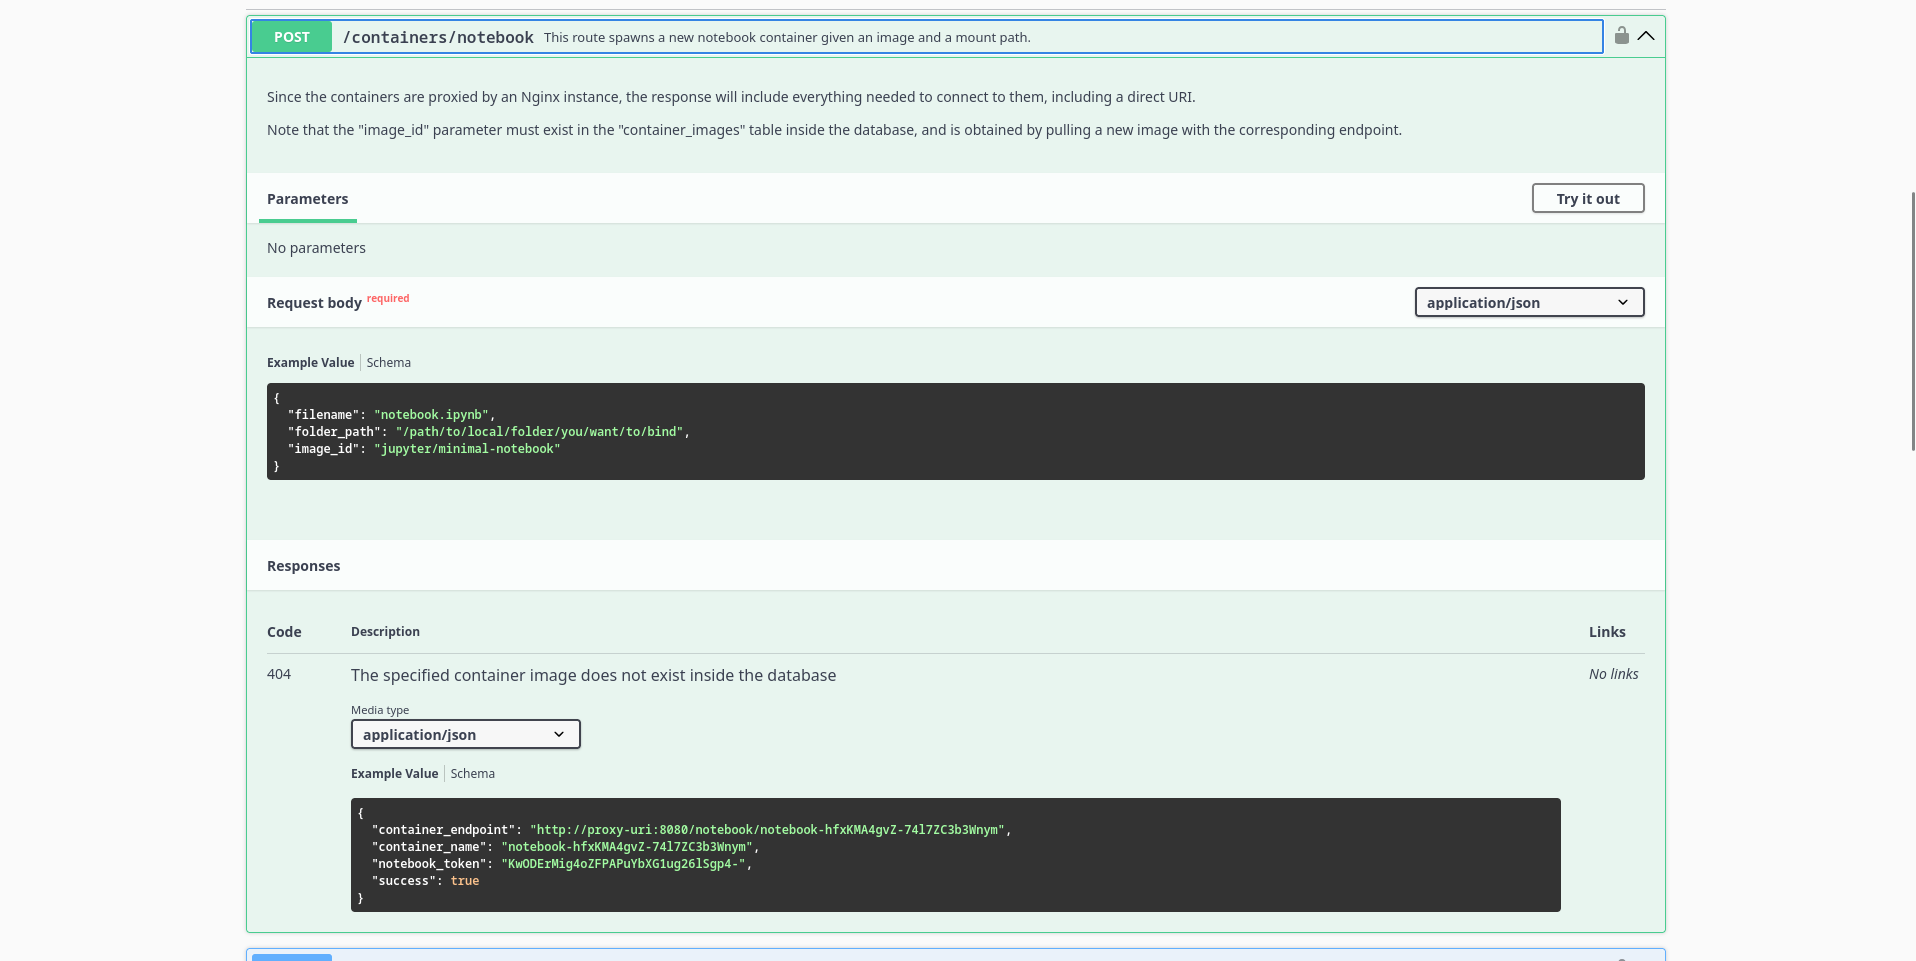
\includegraphics[width=1\textwidth]{files/images/swagger-ui-1.png}
    \caption{Schermata di \textit{Swagger UI} per il modulo \textit{daemon}}
    \label{fig:swagger-ui-daemon}
\end{figure}
\newline
Notare come in figura \ref{fig:swagger-ui-daemon} si possano vedere tutti i metadati che sono stati inseriti usando \textit{utoipa}. 
\newpage
\section{Modellazione del sistema tramite Docker Compose}
Come primo, semplice, modello, usabile anche per \textit{demo} e per capire come i componenti comunicano tra loro, è possibile fare riferimento alla seguente repo\footnote{https://gitlab.com/nextpyter/core}.
\newline
Tramite questa repository è possibile capire il reale funzionamento del \textit{core} di NextPyter su scala ridotta, anche se, in pratica, questa configurazione è già modificabile per essere production-ready, a supporto di deployment più piccoli.
\newline
Il sistema viene modellato tramite Docker Compose nel seguente modo:
\begin{verbatim}
networks:
  daemon-net:
    name: daemon-net

volumes:
  rqlite_data:
  nc_db:
  nc_cfg: 
  nextpyter_binds:
    external:
      true

services:
  config-store:
   image: rqlite/rqlite
   command: -auth /conf/config.json -node-id 1
   networks:
     - daemon-net
   volumes:
     - ./rqlite/config:/conf
     - rqlite_data:/rqlite/file
   ports:
     - 4001:4001

  app:
   depends_on:
     - config-store
   container_name: nextpyter-daemon
   image: emilianomaccaferri/nextpyter-daemon:0.0.1-images-stream-optional-fix
   networks:
     - daemon-net
   volumes:
     - /var/run/docker.sock:/var/run/docker.sock:ro
   environment:
     - RUST_BACKTRACE=1
     - RUST_LOG=trace
     - PROXY_URI=http://localhost:8081
     - RQLITE_USER=tango
     - RQLITE_PASSWORD=test
     - IMAGES_STREAM_NAME=streams:images_data
     - REDIS_URI=redis://queue
     - BIND_VOLUME_PATH=/var/lib/docker/volumes/nextpyter_binds/_data
     - ORCHESTRATOR=docker
     - DOCKER_NETWORK=daemon-net
     - CONFIG_STORE_HOST=config-store:4001
      
  proxy:
    image: nginx
    networks:
      - daemon-net
    volumes:
      - ./nginx/proxy.conf:/etc/nginx/conf.d/proxy.conf
      - ./nginx/oauth:/etc/nginx/conf.d/oauth
      - ./nginx/nginx.conf:/etc/nginx/nginx.conf
      - ./nginx/js:/etc/nginx/js
    ports:
      - 8081:14000
    depends_on:
      - auth
      - app
      - swagger-ui

  swagger-ui:
    image: swaggerapi/swagger-ui
    networks:
      - daemon-net

  pagletto:
    container_name: pagletto
    image: emilianomaccaferri/nextpyter-pagletto:0.0.1
    depends_on:
      - queue
    environment:
      - NOTIFICATION_GROUP=builders
      - CONSUMER_NAME=notifier-1
      - BLOCK_TIME=6000 # how much should the consumer block for?
      - STREAM_NAME=streams:images_data
      - REDIS_URI=redis://queue
      - ITEM_COUNT=10
      - DEAD_KEY_EXPIRY=11000 # how much time should pass before autoclaiming messages?
      - RQLITE_USER=tango
      - RQLITE_PASSWORD=test
      - RQLITE_URI=config-store:4001
      #- RUST_LOG=trace
    networks:
      - daemon-net
    volumes:
      - /var/run/docker.sock:/var/run/docker.sock:ro      
  
  queue:
    image: valkey/valkey:7.2-bookworm
    networks:
      - daemon-net
    depends_on:
      - auth # needed so the resolver knows where to point

  auth:
    build:
      context: .
      dockerfile: ./keycloak/Dockerfile
      network: host
    depends_on:
      auth_db:
        condition: service_healthy
    entrypoint: ["/opt/keycloak/bin/kc.sh", "start-dev"]
    environment:
      - KC_DB=postgres
      - KC_DB_URL=jdbc:postgresql://auth_db:5432/keycloak
      - KC_DB_USERNAME=test
      - KC_DB_PASSWORD=test1
      - KC_HOSTNAME=localhost
      - KC_HOSTNAME_PORT=8080
      - KC_HOSTNAME_STRICT=false
      - KC_HOSTNAME_STRICT_HTTPS=false
      - KEYCLOAK_ADMIN=admin
      - KEYCLOAK_ADMIN_PASSWORD=admin
    ports:
      - 8080:8080
    networks:
      - daemon-net

  auth_db:
    image: postgres
    environment:
      - POSTGRES_DB=keycloak
      - POSTGRES_USER=test
      - POSTGRES_PASSWORD=test1
    healthcheck:
      test: ["CMD-SHELL", "pg_isready -d keycloak -U test"]
      interval: 10s
      timeout: 5s
      retries: 5
    networks:
      - daemon-net

\end{verbatim}

Tramite l'utilizzo di un \textit{Docker network}, quindi, sarà possibile isolare i componenti del \textit{core} e fare in modo che questi comunichino tra di loro usando esclusivamente i nomi \textit{DNS} dei container.
\newpage
\subsection{Limiti di questo \textit{deployment}}
Questo modo di eseguire \textit{core}, seppur funzionante al 100\%, ha una particolarità che può risultare scomoda nel suo \textit{setup} e manutenzione: il volume al quale i \textit{notebook} dovranno fare riferimento dovrà essere \textbf{condiviso} con tutti gli altri container che dovranno accedere ai dati sui quali i notebook opereranno, in questo caso \textbf{un'eventuale installazione di \textit{Nextcloud}}. Per come sono implementati (si fa riferimento al \textit{driver} standard) i volumi in Docker, questo può generare problemi in termini di permessi di accesso ai file, poiché saranno impostati in base al container che genera tali file. Una soluzione potrebbe essere quella di mappare l'utente all'interno di tutti i container a quello dell'host che esegue il Docker \textit{daemon}, risolvendo effettivamente il problema dei permessi, ma introducendone altri riguardanti la gestione e la flessibilità di questo approccio \cite{owasp-docker}.
\newline
Un'effettiva soluzione ai problemi di sicurezza potrebbe essere l'utilizzo di \textit{Podman}\footnote{https://podman.io/}, un'alternativa OCI-compliant\footnote{https://opencontainers.org/} \textit{daemonless} a Docker. Poiché OCI-compliant, quindi aderente agli stessi standard di containerizzazione che Docker usa, Podman può essere effettivamente utilizzato come \textit{drop-in} replacement a Docker, senza cambiare nulla riguardante la configurazione di NextPyter.
\newline
Rimane, inoltre, il problema derivante da \textit{Docker-in-Docker} che, sebbene è particolarmente limitato, può comunuque generare problemi in caso \textit{daemon} presentasse delle vulnerabilità.
\newline
Questi motivi, assieme ad altri citati precedentemente nei capitoli di introduzione, hanno portato alla migrazione del progetto su Kubernetes.
\newpage
\section{NextPyter su Kubernetes}
Kubernetes è una piattaforma \textit{open-source} per l'orchestrazione di container, progettata per automatizzare il deployment, la gestione e lo scaling di applicazioni containerizzate raggruppate in un \textit{cluster}. Un cluster cluster sarà composto da svariati nodi (fisici o virtualizzati, sostanzialmente i server su cui verranno eseguiti i container), offrendo funzionalità come il bilanciamento del carico, il monitoraggio dello stato delle applicazioni, la gestione della scalabilità automatica e l'auto-riparazione dei container qualora questi presentassero errori. La particolarità di Kubernetes è l'approccio dichiarativo alla configurazione dell'infrastruttura: tramite file \textit{YAML} viene definito lo stato desiderato per i componenti di un'applicazione (ad esempio, quanti container devono essere in esecuzione) e il sistema si occupa di mantenere questo stato in modo autonomo. 
\newline
\newline
Oltre a queste funzionalità, Kubernetes offre degli \textit{standard} per quanto riguarda l'implementazione di molti componenti che lo compongono, come \textit{CNI} (\textit{Container Network Interface}), \textit{CSI} (\textit{Container Storage Interface}) e simili.
\newline
In altre parole, dati questi standard completamente \textit{open source} è possibile creare dei cosiddetti \textit{driver} personalizzati che li andranno ad implementare, rendendo estremamente facile l'estensione di nuove tecnologie all'interno di \textit{cluster} Kubernetes. Ad esempio, è possibile implementare in maniera completamente trasparente ai container che ne faranno utilizzo, lo \textit{storage} dei container mediante \textit{iscsi}\footnote{https://github.com/kubernetes-csi/csi-driver-iscsi}, abilitando, di fatto, tutti i concetti che quest'ultimo introduce, senza modificare nulla nel comportamento dei container e di come questi accedono allo \textit{storage}. Kubernetes, quindi, \textit{astrae} completamente la gestione di \textit{network}, \textit{storage} e molto altro e la delega a determinati \textit{driver}, che, rispettando l'interfaccia data, potranno offrire funzionalità estremamente personalizzabili e in maniera altamente modulare.
\newline
NextPyter fruirà di queste particolarità per andare a realizzare \textit{deployment} altamente personalizzabili e scalabili in maniera estremamente semplice, integrandosi con Kubernetes in modo completamente trasparente a container e utenti finali.
\newpage
\subsection{Utilizzo di \textit{kube-rs} per l'interfaccia con Kubernetes}
Il \textit{trait} \verb|Orchestrator|, discusso nella sezione \ref{axum-orchestrator} utilizza, come già detto, \textbf{Bollard} per interfacciarsi con Docker (o Podman), mentre fa utilizzo della libreria \textit{kube-rs} per comunicare con i componenti di "amministrazione" di un cluster Kubernetes.
\subsection{Rimozione di \textit{pagletto} per questa configurazione}
Kubernetes supporta automaticamente il download di immagini di container quando non sono presenti nel sistema, pertanto il modulo \textit{pagletto}, non è più necessario per un deployment Kubernetes.
\newline
Ciò che rimane, però, sarà la parte di configurazione distribuita che permetterà di memorizzare le immagini disponibili su NextPyter, mentre \textit{pagletto} è stato sostituito con il trait \verb|Waitable|, così definito:
\begin{verbatim}
use std::fmt::Display;

use axum::async_trait;
use super::OrchestratorError;

#[async_trait]
pub trait Waitable {
    type StatusEnum: ToString;
    async fn wait(&self, fields: &str, status: Self::StatusEnum) 
        -> Result<(), OrchestratorError>;
}

pub struct WaitableKubernetesResource<R> {
    pub resource: R,
}
impl<R> WaitableKubernetesResource<R> {
    pub fn new(resource: R) -> Self {
        WaitableKubernetesResource {
            resource
        }
    }
}

\end{verbatim}

Notare come è stato introdotto anche il tipo \verb|WaitableKubernetesResource<R>|. Questa struttura dati sarà usata come \textit{helper} per poter implementare \textit{trait} su tipi derivanti da altre librerie, cosa che non è possibile fare \textit{direttamente} in Rust per via di come è stato pensato il linguaggio. In particolare, quindi, ogniqualvolta si vorrà implementare il trait \verb|Waitable| su un tipo di un'altra libreria, come \verb|Pod| di \textit{kube-rs}, lo si dovrà \textit{wrappare} in \verb|WaitableKubernetesResource<R>|, come in questo esempio:
\begin{verbatim}
#[async_trait]
impl Waitable for WaitableKubernetesResource<Api<Pod>> {

    type StatusEnum = PodStatusEnum;

    async fn wait(&self, fields: &str, resource_status: Self::StatusEnum)
    -> Result<(), OrchestratorError> {
        let wp = WatchParams::default().fields(&fields)
        .timeout(std::env::var("K8S_WATCH_TIMEOUT")
            .unwrap_or("10".to_string()).parse().unwrap_or(10)
        );

        let mut stream = self.resource.watch(&wp, "0").await?.boxed();

        while let Some(status) = stream.try_next().await? {
            match status {
                WatchEvent::Modified(o) => {
                    if let Some(s) = o.status.as_ref(){
                        let phase = s.phase.clone().unwrap_or_default();
                        if phase.eq(&resource_status.to_string()) {
                            break;
                        }
                    }
                }
                WatchEvent::Error(e) => {
                    return Err(e.into())
                }
                _ => {}
            }
        }
        Ok(())
    }
}

\end{verbatim}
Ciò che fa il trait \verb|Waitable|, sostanzialmente, è aspettare che una risorsa Kubernetes venga messa nello stato che viene passato al metodo \verb|wait|, a significare che la risorsa è pronta per essere usata.
\newline
Questa funzionalità è ampiamente utilizzata nella \textit{codebase} di NextPyter, come in questo esempio:
\begin{verbatim}
async fn start_notebook_container(
    &self, 
    container_name: &str,
    container_image: &str,
    container_command: Vec<&str>,
    volume_name: &str,
    filename: Option<&str>,
) -> Result<String, OrchestratorError>{

    let pod_api: Api<Pod> = Api::namespaced(
        self.runtime.clone(), 
        &get_k8s_namespace()
    );

    // dettagli omessi per chiarezza
    let pod_definition: Pod = serde_json::from_value(json!({...})?;

    pod_api
        .create(&PostParams::default(), &pod_definition)
        .await?;

    let waitable_pod = WaitableKubernetesResource::new(pod_api);

    // https://kubernetes.io/docs/concepts/workloads/pods/pod-lifecycle/#pod-phase
    waitable_pod.wait(
        &format!("metadata.name={}", container_name), 
        PodStatusEnum::Running
    )
    .await?;
        
    Ok(build_notebook_uri(container_name, filename))

}
\end{verbatim}
Come anticipato, si crea l'oggetto che si vuole "aspettare" e lo si \textit{wrappa} nel tipo \verb|WaitableKubernetesResource|. A questo punto, basta chiamare il metodo \verb|wait|, al quale si passerà lo stato che si vorrà "aspettare" (in questo caso si vuole attendere che il \verb|Pod| parta, quindi si utilizza \verb|PodStatusEnum::Running|).
\newline
Anche questa semplice interfaccia permette di standardizzare il framework di NextPyter, rendendolo molto più mantenibile.
\newpage
\subsection{\textit{ServiceAccount} per il modulo \textit{daemon}}
Sebbene la \textit{codebase} del modulo \textit{daemon} sia completamente trasparente, in termini di utilizzo, rispetto all'orchestratore in uso, Kubernetes è \textit{molto} diverso da Docker in termini di architettura.
\newline
In particolare, Kubernetes è composto da tre principali moduli:
\begin{itemize}
    \item \textbf{kube-scheduler}: componente incaricato di gestire dove \textit{e come} posizionare i container all'interno di un cluster;
    \item \textbf{kube-controller-manager}: gestisce il ciclo di vita delle risorse all'interno di un cluster, controllando quando queste non sono più raggiungibili o quando necessitano di attenzione;
    \item \textbf{etcd}: componente che permette di memorizzare la configurazione del cluster in maniera distribuita e \textit{fault-tolerant}.
\end{itemize}
Per poter interagire con questi componenti, Kubernetes rende disponibile un quarto componente, \textbf{kube-apiserver}, che espone una API HTTP tramite la quale è possibile interagire in maniera programmatica con il cluster.
\newline
Per accedere a questa API in maniera programmatica, è necessario creare un \textit{ServiceAccount}\footnote{https://kubernetes.io/docs/concepts/security/service-accounts/}, con terminologia particolarmente simile a quella usata in \textit{OAuth2}, per poter regolare gli accessi alle risorse esposte da \textit{kube-apiserver}.
\newline
Un \textit{service account} è un tipo di credenziale che permette di far accedere container \textit{interni} al cluster a \textit{kube-apiserver}. In questa maniera, i \textit{pod} a cui sono associati determinati \textit{service account} potranno identificarsi verso il cluster e accedere alle risorse per cui hanno determinati permessi.
\newline
A differenza di Docker, Kubernetes necessita che vengano create questo genere di credenziali per accedere alla API HTTP che esso espone, per aggiungere un layer di sicurezza addizionale.
\newline
Creare un \textit{service account} è particolarmente semplice:
\begin{verbatim}
apiVersion: v1
kind: ServiceAccount
metadata:
  name: notebook-creator-sa
  namespace: nextpyter-core
\end{verbatim}
Di base, un \textit{service account} non ha alcun permesso, pertanto è necessario creare un \textit{Role}:
\begin{verbatim}
apiVersion: rbac.authorization.k8s.io/v1
kind: Role
metadata:
  namespace: nextpyter-core
  name: notebook-creator
rules:
- apiGroups: [""] # "" indicates the core API group
  resources: ["pods"]
  resourceNames: ["notebook-*"]
  verbs: ["create", "watch", "list", "get", "delete"]
\end{verbatim}
Il \textit{role} raccoglie determinati permessi che verranno associati ad un \textit{service account} mediante un \textit{role binding}:
\begin{verbatim}
kind: RoleBinding
apiVersion: rbac.authorization.k8s.io/v1
metadata:
  name: notebook-creator-binding
  namespace: nextpyter-core
subjects:
  - kind: ServiceAccount
    name: notebook-creator-sa
    namespace: nextpyter-core
roleRef:
  kind: Role
  name: notebook-creator
  apiGroup: rbac.authorization.k8s.io
\end{verbatim}
In questo modo, i \textit{pod} che avranno questo \textit{service account} associato potranno interrogare \textbf{kube-apiserver} per \textit{creare, osservare, elencare, rimuovere e ottenere informazioni} riguardanti le risorse che contengono la stringa \verb|notebook-| all'interno del proprio nome.
\newline
Associare un \textit{service account} a un \textit{pod} è immediato:
\begin{verbatim}
apiVersion: apps/v1
kind: Deployment
metadata:
  name: daemon-deployment
  namespace: nextpyter-core
spec:
  replicas: 3
  selector:
    matchLabels:
      app: daemon
  template:
    metadata:
      labels:
        app: daemon
    spec:
      # qua viene mappato il service account
      serviceAccountName: notebook-creator-sa 
      containers:
      - name: daemon
        image: emilianomaccaferri/nextpyter-daemon:0.0.1-subpath
        imagePullPolicy: IfNotPresent
        # altri dettagli omessi per brevità... 
\end{verbatim}
In questa maniera, quindi, è possibile fare comunicare \textit{daemon} con \textit{kube-apiserver} un po' come veniva fatto tramite l'apporccio \textit{DinD}, senza però ricorrere a soluzioni che potrebbero causare vulnerabilità di privilege escalation all'interno del sistema, poiché viene esplicitamente dichiarato ciò che un container può fare quando andrà a contattare l'\textit{apiserver} di Kubernetes.
\newline
Notare come \textit{daemon} venga immesso nel cluster tramite un \textit{Deployment}, un particolare costrutto Kubernetes che permette di creare delle repliche \textit{stateless} di un'applicazione.
\newline
La creazione di un cluster con NextPyter verrà comunque dettagliata maggiormente tra qualche sezione.
\newpage
\subsection{RQLite su Kubernetes}
Il deployment di RQLite su Kubernetes necessita di particolari accortezze per garantire la corretta replicazione e conservazione dei dati.
\newline
\subsubsection{\textit{StatefulSets}}
Uno \textit{StatefulSet} è un particolare tipo di risorsa che viene usata in un cluster Kubernetes per creare una serie di \textit{pod} identici, ma non intercambiabili (a differenza di un \textit{Deployment}).
\newline
Uno \textit{StatefulSet} permette di mantenere, quindi, persistenza "deterministica" anche in caso i \textit{pod} che fanno parte di tale \textit{StatefulSet} siano soggetti a problematiche.
\newline
Il classico caso d'uso per questo genere di risorsa è quello dei database distribuiti, come \textit{RQLite}: applicazioni di questo tipo, generalmente, mantengono relazioni di subordinazione tra i componenti che stabiliscono principalmente l'ordine nel quale i dati sul database vengono inseriti.
\newline
I componenti di \textit{RQLite}, per funzionare correttamente, hanno bisogno di persistenza a livello di nomi di container e a livello di storage, rendendo lo \textit{StatefulSet} la risorsa perfetta da utilizzare in questo caso.
\newline
In particolare, quando i nodi di un cluster \textit{RQLite} vanno online, questi registrano la loro identità verso i \textit{leader} del cluster, eletto tramite protocollo \textit{raft}. A questo punto, tutte le scritture sul database passeranno per i nodi \textit{leader}, che terranno un registro degli eventi che accadono sul cluster stesso.
\newline
Se uno dei nodi \textit{RQLite} va offline, Kubernetes provvederà a farlo tornare online al più presto. Quando questo tornerà online, la sua identità dovrà essere ripristinata completamente e che i dati che il nodo gestiva precedentemente vengano ad esso riassociati. Lo \textit{StatefulSet} farà esattamente questo: quando il \textit{pod} precedentemente andato offline tornerà operativo verrà riassociato alla sua identità e al \textit{volume} dei dati che gestiva precedentemente all'arresto.

\subsubsection{Storage: PV, PVC e \textit{storage classes}}
Da documentazione\footnote{https://kubernetes.io/docs/concepts/workloads/controllers/statefulset/#limitations}, gli \textit{stateful set} richiedono che i dati riguardanti i \textit{pod} che lo compongano vengano memorizzati utilizzando dei \textit{persistent volumes} (PV), che potranno essere creati manualmente o tramite \textit{storage classes}, che verranno dettagliate tra poco.
\newline
Un \textit{persistent volume}, in Kubernetes, rappresenta, in breve, un dispositivo di memorizzazione dati fruibile dal cluster. Questa particolare risorsa permette di astrarre completamente i dettagli dell'implementazione di questo dispositivo di storage (che potrà essere \textit{iscsi}, \textit{Ceph-like}, persino \textit{bucket S3}, ...) dal cluster, in maniera da rendere trasparente l'accesso ai dati da parte dei \textit{pod}.
\newline
Per accedere ad un \textit{persistent volume}, un \textit{pod} dovrà fare un \textit{persistent volume \textbf{claim}} (PVC), sostanzialmente una "richiesta" di utilizzo di un \textit{persistent volume}. Vi potrà essere \textbf{al massimo} un PVC per PV, ma a tale PVC potranno fare riferimento tanti \textit{pod} diversi, come in figura \ref{fig:pvc-to-pv}.
\begin{figure}[h]
    \centering
    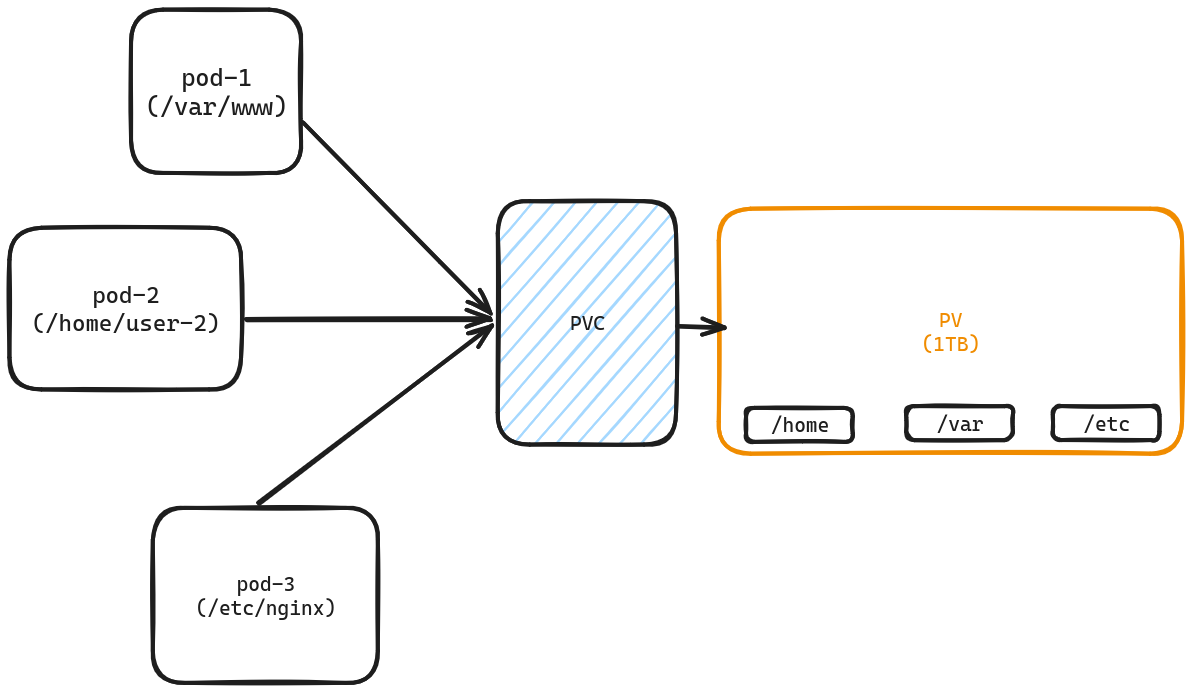
\includegraphics[width=0.75\textwidth]{files/images/pvc-to-pv.png}
    \caption{Funzionamento di PVC e PV}
    \label{fig:pvc-to-pv}
\end{figure}
\newline
In questo modo, tutti i \textit{pod} che fanno riferimento allo stesso PVC "vedranno" lo stesso filesystem, al quale potranno fare modifiche, eventualmente, in simultanea: questo è, sostanzialmente, il motivo per il quale gli \textit{stateful set} richiedono dei \textit{persistent volume} dedicati \textbf{per pod}! In questa maniera, ciascun \textit{pod} farà riferimento ad una porzione di storage completamente indipendente dalle altre, in maniera da accedere ai file senza problemi di concorrenza. Questo concetto è fondamentale quando si devono implementare database distribuiti su Kubernetes. RQLite, infatti, utilizza un log distribuito per replicare i dati sui vari nodi: la richiesta di scrittura arriva sul nodo autoritativo, questo fa partire una transazione distribuita e impone a tutti i nodi di replicare tale scrittura e, quando la maggioranza dei nodi ha finito, la scrittura sarà marcata come "completa". Ora, si supponga che uno dei nodi, che chiameremo \textit{n-1}, del cluster RQLite vada offline e che nel periodo in cui questo non è disponibile vengano effettuate diverse scritture sul cluster. Quando \textit{n-1} tornerà online, controllerà il log distribuito e scriverà, nella sua parte di storage, indipendente dalle altre, i record mancanti.
\newline
Questo meccanismo sarebbe molto più complicato da implementare senza \textit{persistent volume} separati, poiché all'avvio di \textit{n-1}, per prima cosa, questo sovrascriverebbe i record già esistenti (inutilmente). Inoltre, quando più applicazioni fanno riferimento agli stessi file, le logiche di accesso a questi ultimi non sono sempre deterministiche e potrebbero risultare in problemi derivanti da \textit{race condition}, rendendo quasi impossibile il soddisfacimento delle garanzie che un database \textit{ACID} riesce a dare. 
\newline
Il \textit{deployment} di RQLite in NextPyter, quindi, ha la struttura visibile in figura \ref{fig:rqlite-storage-deployment}.
\begin{figure}[h]
    \centering
    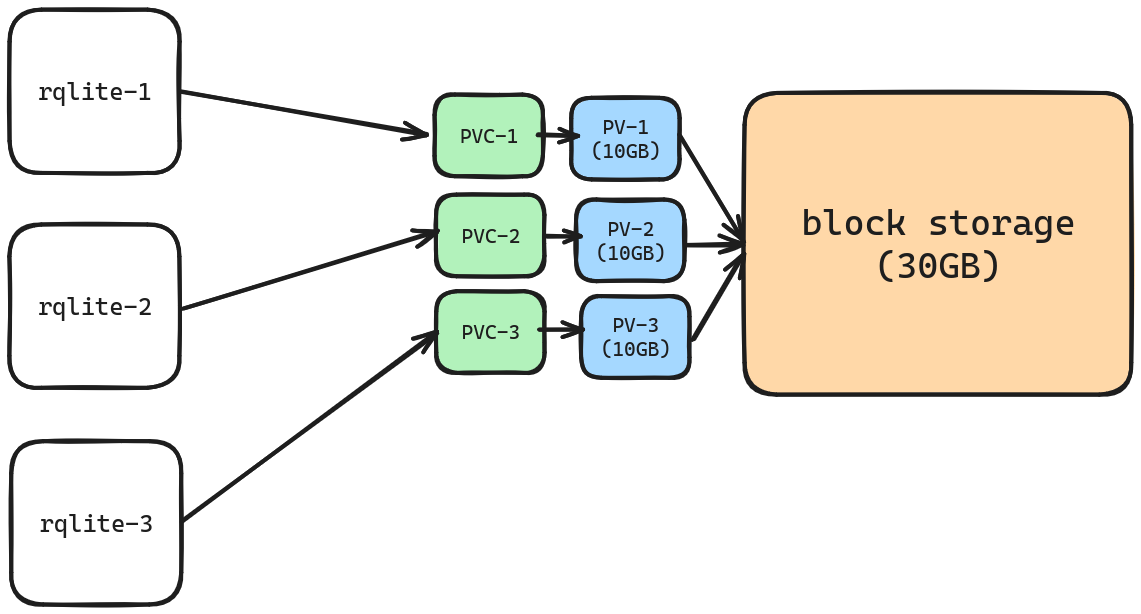
\includegraphics[width=0.75\textwidth]{files/images/rqlite-deployment.png}
    \caption{Schema deployment storage RQLite}
    \label{fig:rqlite-storage-deployment}
\end{figure}
Per gli \textit{stateful set}, quindi, vengono assegnati ai pod dei PV "vuoti" inizialmente, che derivano, generalmente, da un dispositivo a blocchi. Viene riservata, infatti, una capacità di spazio arbitraria che viene data "in prestito" al pod, che la userà per il periodo di durata dello \textit{stateful set}.
\newline
Generalmente, poiché creare \textit{persistent volume} è una pratica abbastanza ripetitiva, è buona norma definire una \textit{storage class}, sostanzialmente un componente che si andrà ad occupare del \textit{provisioning} automatico dei \textit{persistent} volume richiesti da determinati \textit{pod}.
\newline
In questo modo, alla creazione dei pod di uno \textit{stateful set}, questi andranno ad interrogare la \textit{storage class} per richiedere dei \textit{persistent volume}, che verranno automaticamente generati ed assegnati a quest'ultimo.
\subsubsection{OpenEBS}
Una \textit{storage class} richiederà la presenza di un \textit{provisioner}, assimilabile ad un \textit{driver} che si interfaccerà col dispositivo a blocchi dal quale si riserverà lo spazio. A questo pro è stato scelto OpenEBS\footnote{https://openebs.io/}, che permetterà di potersi interfacciare con \textit{pool zfs} per gestire i dati di applicazioni \textit{stateful}.
\newline
In sostanza, quindi, un \textit{pod} di uno \textit{stateful set} farà una "richiesta di spazio" ad una determinata storage class e quest'ultima si interfaccerà direttamente col \textit{provisioner} che creerà PV e PVC richiesti dal \textit{pod}. Configurare questo processo è molto semplice, una volta installato il provisioner:
\begin{verbatim}
apiVersion: storage.k8s.io/v1
kind: StorageClass
metadata:
  name: dynamic-openebs
  namespace: nextpyter-core
parameters:
  recordsize: "128k"
  compression: "off"
  dedup: "off"
  fstype: "zfs"
  poolname: "zfspv-pool"
provisioner: zfs.csi.openebs.io 
\end{verbatim}
Come si può vedere, una \textit{storage class} conterrà tutti i parametri che verranno utilizzati per accedere al \textit{provisioner}, in modo da centralizzarne la configurazione.
\newline
A questo punto, un \textit{pod} dovrà soltanto fare riferimento alla \textit{storage class}:
\begin{verbatim}
apiVersion: apps/v1
kind: StatefulSet
metadata:
  name: rqlite
  namespace: nextpyter-core
spec:
  selector:
    matchLabels:
      app: rqlite 
  # dettagli omessi per brevità...
  volumeClaimTemplates:
  - metadata:
      name: rqlite-file
    spec:
      accessModes: [ "ReadWriteOncePod" ]
      storageClassName: dynamic-openebs # nome della storage class
      resources:
        requests:
          storage: 1Gi # richiesta di storage
\end{verbatim}
Inoltre, l'accesso ad un \textit{persistent volume} potrà essere configurato in vari modi:
\begin{itemize}
    \item \verb|ReadWriteOnce|: il volume può essere acceduto in maniera \textit{read-write} da un singolo \textbf{nodo} (non \textit{pod}!) del cluster;
    \item \verb|ReadOnlyMany|: il volume può essere acceduto in maniera \textit{read-only} da tanti nodi;
    \item \verb|ReadWriteMany|: come il precedente, ma \textit{read-write};
    \item \verb|ReadWriteOncePod|: come \verb|ReadWriteOnce|, ma per \textbf{singolo pod}, rendendo l'accesso al volume molto più granulare. 
\end{itemize}
\newpage
\subsection{Gestione storage dei notebook}
La questione della gestione \textit{indipendente} e "\textit{sicura}" dei volumi dei notebook è già stata evidenziata come requisito critico di NextPyter, pertanto, in questa sezione, si va a documentare la sua implementazione mediante \textit{Datashim}\footnote{https://datashim.io/}.
\newline
Come abbiamo già visto in precedenza, la gestione dei volumi è di vitale importanza per una serie di aspetti di sicurezza molto critici ed è di difficile modellazione con un semplice \textit{deployment} tramite Docker Compose. Sfruttando le interfacce che Kubernetes ha da offrire, però, è stato possibile realizzare un sistema che permetta l'accesso ai dati in maniera sicura da parte dei notebook, senza dover specificare permessi speciali e quant'altro.
\newline
Datashim è un progetto open-source che ha come scopo quello di semplificare drasticamente la gestione dei PVC per \textit{pod} non stateful all'interno di un cluster Kubernetes, permettendo di astrarre, tramite il concetto di \verb|Dataset|, quello che è la gestione e il provisioning di PVC.
\subsubsection{Supporto a \textit{bucket S3}}
L'idea alla base di NextPyter è quella della modularità ed indipendenza dei componenti nella maniera più estrema possibile e lo \textit{storage} è quello più difficile da astrarre, per via della coesione che quest'ultimo ha con il sistema sottostante.
\newline
NextPyter su Kubernetes, però, è una piattaforma completamente \textit{storage agnostic}, data la estrema astrazione che Kubernetes è in grado di offrire grazie alla sua potente API. In particolare, a prova di quanto detto, si è voluto portare il concetto di \textit{"storage-agnosticness"} all'estremo, offrendo supporto a \textit{bucket S3} completamente dislocati dall'infrastruttura fisica su cui si trova il cluster \textit{Kubernetes}.
\newline
Ciò che si è voluto realizzare è visibile in figura \ref{fig:s3-bucket}
\begin{figure}[h]
    \centering
    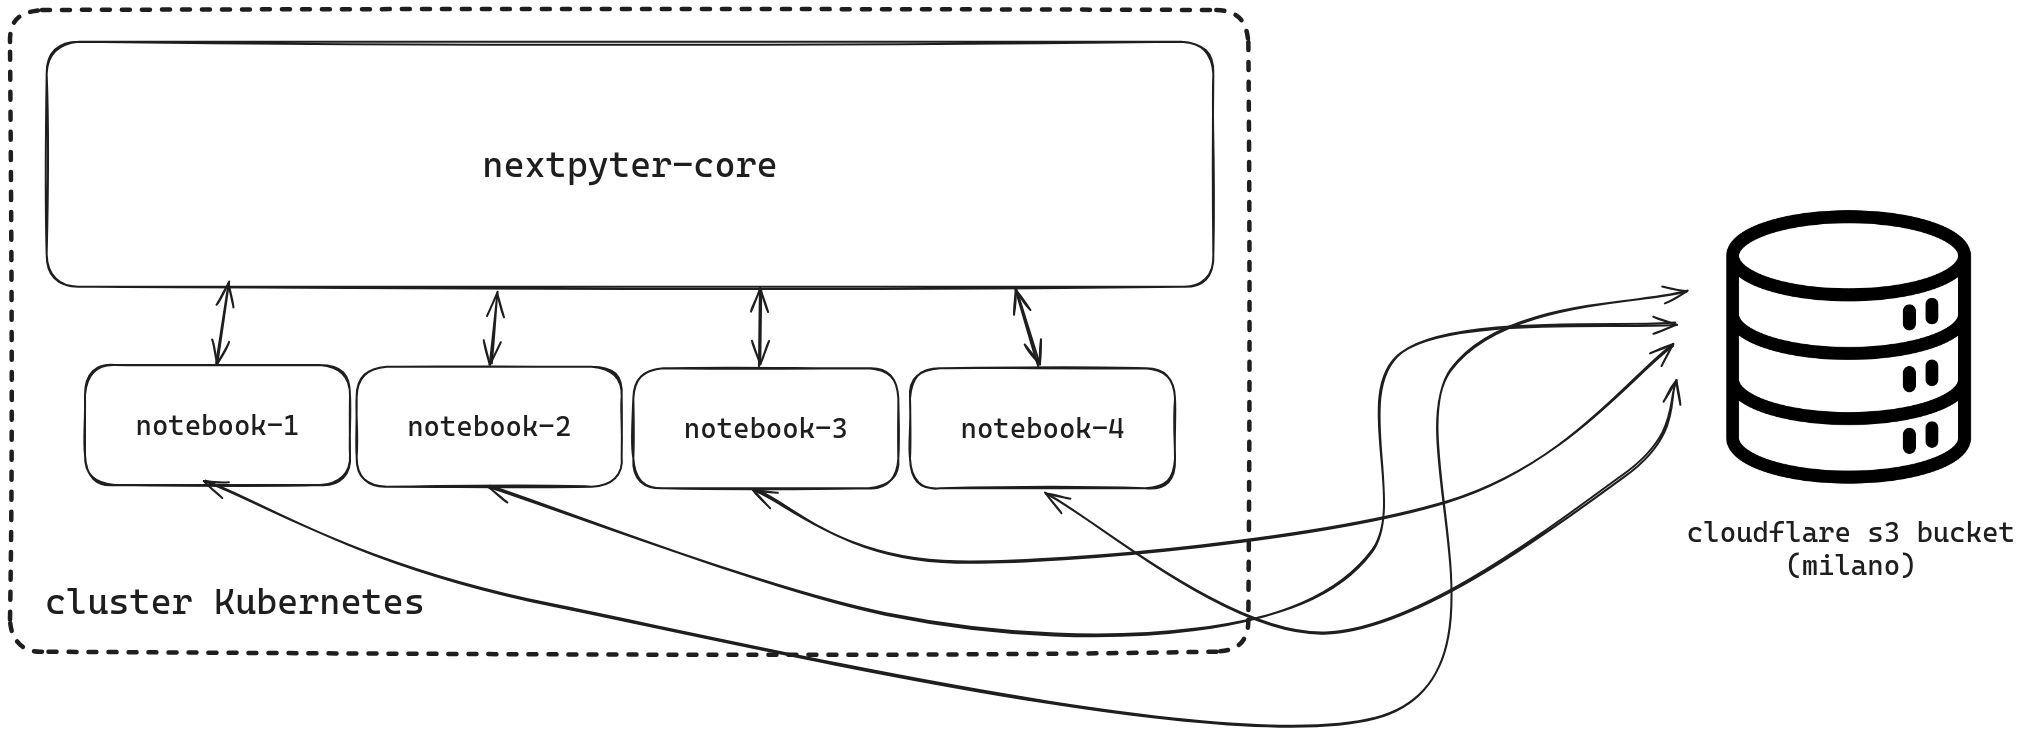
\includegraphics[width=1\textwidth]{files/images/s3-bucket.png}
    \caption{Storage notebook completamente decentralizzato tramite bucket S3}
    \label{fig:s3-bucket}
\end{figure}
In sostanza, i notebook vedranno i loro dati risiedere su un bucket S3 in una location "fisica" completamente diversa dalla loro, per giunta su un servizio \textit{managed} esterno, in modo da azzerare completamente la complessità di gestione di questi ultimi.
\newline
Tramite \textit{Datashim} è possibile configurare tutto questo in maniera estremamente semplice:
\begin{verbatim}
apiVersion: datashim.io/v1alpha1
kind: Dataset
metadata:
  name: nextpyter-notebook-data
  namespace: nextpyter-core
spec:
  local:
    storage:
      type: object
      access:
        accessKeyId: valore-accessKeyId
        secretAccessKey: valore-secretAccessKey
        endpoint: endpoint
        bucketName: nome-bucket

\end{verbatim}
In questo modo, Datashim creerà un PV che rappresenterà il bucket S3 configurato, che sarà accessibile in maniera completamente trasparente dai \textit{pod} come un PVC. Il modulo \textit{daemon}, infatti, farà riferimento al \textit{dataset} appena creato per accedere al bucket in questione:
\begin{verbatim}
let split: Vec<&str> = volume_name.split(":").collect();
// volume_name è, ad esempio: "nome-dataset:/sottocartella/esempio"
// ...
let pod_definition: Pod = serde_json::from_value(json!({
    "apiVersion": "v1",
    "kind": "Pod",
    "metadata": { 
        // ...
        "labels": {
            "dataset.0.id": split[0],
            "dataset.0.useas": "mount",
            "taint": "nextpyter-notebook",
        }
    },
    "spec": {
        // ... 
        "volumes": [
            {
                "name": "notebook-volume",
                "persistentVolumeClaim": {
                    "claimName": split[0]
                }
            }
        ],
        "containers": [{
            // ...
            "volumeMounts": [
                {
                    "mountPath": "/home/nextpyter",
                    "name": "notebook-volume",
                    "subPath": split[1],
                }
            ],
            // ...
            ]
        }] 
    }
}))?;

pod_api
    .create(&PostParams::default(), &pod_definition)
    .await?;
\end{verbatim}
In questo modo, i notebook potranno fruire in maniera completamente trasparente delle funzionalità del dataset appena creato con Datashim, riferendosi a quest'ultimo mediante l'utilizzo di una \textit{label} e dei campi \textit{claimName} e \textit{subPath} della configurazione dei volumi del \textit{pod}.
\newline
Ovviamente questa non è l'unica configurazione supportata, ovviamente, infatti è possibile creare, con altrettanta facilità, il supporto a storage basato su \textit{NFS}\footnote{https://ubuntu.com/server/docs/network-file-system-nfs}, poiché Datashim lo supporta nativamente. È stata scelta volutamente questa configurazione per dimostrare l'estrema elasticità della piattaforma, anche in termini di tipo di storage. 
\newpage
\subsection{Helm per semplificare il deploy di NextPyter}
Sebbene completo e funzionante, NextPyter è composto da tante \textit{moving parts}, che vanno configurate e di cui va effettuato il \textit{deployment singolarmente}: i moduli \textit{core}, la gestione degli \textit{stateful sets} di cui abbiamo parlato precedentemente, la creazione dei \textit{dataset} di Datashim, la configurazione di NGINX, ...
\newline
Vi sono molte cose da fare e sarebbe interessante trovare un modo per "pacchettizzare" tutte queste operazioni in un singolo "blocco" ed eseguirle tutte insieme in automatico, magari personalizzando alcuni aspetti. Questo è esattamente il caso d'uso di \textit{Helm}, uno strumento che permette di gestire le applicazioni che andranno eseguite sui cluster Kubernetes (e le loro dipendenze) modellandole come "pacchetti" facilitando la definizione, l'installazione e l'aggiornamento di queste ultime. I "pacchetti" Helm sono chiamati \textit{charts} e contengono template YAML predefiniti per descrivere in modo dichiarativo le configurazioni delle varie risorse come \textit{pod}, \textit{stateful set} e quant'altro. Questo permette di gestire facilmente le dipendenze tra componenti software e di automatizzare i processi di rilascio, promuovendo la riproducibilità e la consistenza tra ambienti. Helm, inoltre, adotta un sistema di versionamento che facilita la gestione dei cicli di vita delle applicazioni, con la possibilità di eseguire rollback rapidi a versioni precedenti in caso di errori. L’utilizzo di repository di \textit{charts}, sia pubbliche che private, incoraggia il riutilizzo di configurazioni e contribuisce alla standardizzazione dei deployment in ambienti di produzione e sviluppo.
\newline
\subsubsection{Struttura della \textit{Helm chart} di NextPyter}
La \textit{Helm chart}\footnote{https://gitlab.com/nextpyter/helm-chart} di NextPyter è stata creata, per l'appunto, per semplificare il deployment di tutte le componenti che vanno a rendere utilizzabile la piattaforma.
\newline
Nella cartella \textit{templates}\footnote{https://gitlab.com/nextpyter/helm-chart/-/tree/main/templates} sono definite tutte le risorse che andranno inserite nel cluster Kubernetes, sottoforma di, appunto, \textit{template Go}, sostanzialmente dei file che vengono interpretati da \textit{Helm} nei quali verranno sostituite le variabili definite con dei valori stabiliti a monte.
\newline
Questo, ad esempio, è il \textit{template} che fa riferimento alla creazione della \textit{storage class} che servirà agli \textit{stateful set} per operare correttamente:
\newpage
\begin{verbatim}   
{{- if eq .Values.zfs true }}
apiVersion: storage.k8s.io/v1
kind: StorageClass
metadata:
  name: dynamic-openebs
  namespace: {{ include "nextpyter.core-namespace" . }}
parameters:
  recordsize: "128k"
  compression: "off"
  dedup: "off"
  fstype: "zfs"
  poolname: "zfspv-pool"
provisioner: zfs.csi.openebs.io
{{- if .Values.storageNodes }}
allowedTopologies:
- matchLabelExpressions:
  - key: kubernetes.io/hostname
    values: 
      {{- range .Values.storageNodes | default nil }}
      - {{ . }}
      {{- end}}
{{- end }}
{{- else }}
apiVersion: storage.k8s.io/v1
kind: StorageClass
metadata:
  name: dynamic-openebs
  namespace: {{ include "nextpyter.core-namespace" . }}
allowVolumeExpansion: true
parameters:
  storage: "lvm"
  volgroup: "lvmvg"
provisioner: local.csi.openebs.io
{{- if .Values.storageNodes }}
allowedTopologies:
- matchLabelExpressions:
  - key: kubernetes.io/hostname
    values: 
      {{- range .Values.storageNodes | default nil }}
      - {{ . }}
      {{- end}}
{{- end }}
{{- end}}
\end{verbatim}
All'interno della \textit{chart}, inoltre, si troverà un file chiamato \verb|values.yaml|, che potrà essere utilizzato per personalizzare l'installazione di NextPyter mediante Helm.
\newline
La struttura del file è molto semplice ed intuitiva:
\begin{verbatim}
# datashim storage configuration
storage:
  type: object
  access:
    accessKeyId: accessKeyId
    secretAccessKey: secretAccessKey
    endpoint: endpoint
    bucketName: bucket

# NGINX proxy configuration  
proxy: 
  use_keycloak: false
  external_uri: https://app.test.com
  replicas: 5
  # utilizzabili solo se use_keycloak: true
  # introspection_endpoint: ...
  # token_endpoint: ...
  # oauth_client_id: client_name
  # oauth_client_secret: client_secret
  service:
    # può essere anche ClusterIP
    type: NodePort
    hostPort: 34000

rqlite:
  replicas: 3
  username: tango
  password: test

daemon:
  replicas: 3

storageNodes:
    - node1
    - node2
zfs: false
core_namespace_name: nextpyter-core

\end{verbatim}
Nota: la proprietà \verb|storageNodes| permette di definire una serie di nodi che offriranno funzionalità di \textit{storage}, sostanzialmente indicherà i nodi che accoglieranno "fisicamente" i volumi degli \textit{stateful sets}. Se non viene impostato, \textbg{tutti i nodi verranno considerati come storage nodes}!
\newline
Per installare NextPyter utilizzando la Helm chart, basterà clonare la repository ed eseguire il comando:
\begin{verbatim}
    helm install nextpyter -f values.yaml .
\end{verbatim}
In questo modo verrà applicata la configurazione scelta e, in maniera estremamente semplice, NextPyter sarà installato sul cluster Kubernetes di riferimento.
\newpage
\chapter{Conclusioni e sviluppi futuri}
NextPyter si pone come obiettivo la creazione di una piattaforma che faciliti l'accesso alle risorse computazionali in ambiti accademici e non, permettendo, inoltre, alle figure responsabili della gestione di quest'ultima, di poter lavorare con tecnologie all'avanguardia e modulari, garantendo facilità di sviluppo e manutenzione del progetto stesso.
\newline
La tesi aveva come scopo quello di descrivere il funzionamento del \textit{core} di NextPyter, modulo che al momento è completo e funzionante, ma verranno effettuati ultieriori sviluppi per poter adeguare totalmente la piattaforma, comprendendo, quindi, Nextcloud e altre tecnologie di supporto.
\newline
Sono state effettuate due pubblicazioni scientifiche\cite{nextpyter-work-1}\cite{nextpyter-work-2} riguardo NextPyter, a dimostrazione che il progetto è in continua evoluzione.

\section{Sviluppi futuri}
Gli sviluppi futuri includeranno sicuramente il supporto ad un'autenticazione "offline" delle richieste, liberandosi quindi del supporto dell'\textit{introspection endpoint} nell'approccio descritto in \ref{reverse-proxy-oauth}, in modo da garantire un'autenticazione più veloce e che genera meno traffico all'interno del sistema. Ciò che si vuole implementare, in particolare, è una verifica crittografica a livello di \textit{application gateway}, dato che i token che viaggiano nel sistema sono \textit{JWT}, sfruttando le \textit{JWK}\footnote{https://datatracker.ietf.org/doc/html/rfc7517} esposte da Keycloak.
\newline
Altre migliorie verranno integrate per quanto riguarda lo \textit{scheduling} dei pod, infatti è già in creazione il supporto per integrare pod che necessitano di essere GPU-accelerated, che verranno \textit{schedulati} su nodi specifici (con GPU, per l'appunto). Per ora si mira a supportare GPU NVIDIA, ma è già stata individuata una modalità per integrare anche nodi che montano GPU AMD, a supporto di cluster più eterogenei.
\bibliographystyle{unsrt}
\bibliography{main}
\end{document}
